\tableofcontents

\pagebreak
\renewcommand{\listfigurename}{Índice de Figuras}
\listoffigures
\pagebreak
\renewcommand{\listtablename}{Índice de Tablas}
\listoftables
\pagebreak

\pagenumbering{arabic}

%\mainmatter
\addtocontents{toc}{\protect\setcounter{tocdepth}{2}}

\chapter{INTRODUCCIÓN}\label{capitulo:INTRODUCCION}
Este trabajo tiene la finalidad de obtener un diseño preliminar de la geometría
de los sistemas de intercambio de gases del Motor Rotativo de Combustión a
Volumen Constante (MRCVC,~\parencite{toth}), con el objetivo general de
maximizar la eficiencia del sistema en un rango de velocidades del motor.
%

El MRCVC es un proyecto que surgió en la Universidad Nacional del Comahue,
presentado por el Ing. Jorge A. Toth en el año 1996 al Instituto Nacional de
la Propiedad Industrial y patentado en el año 1999.

\begin{figure}
    \centering
    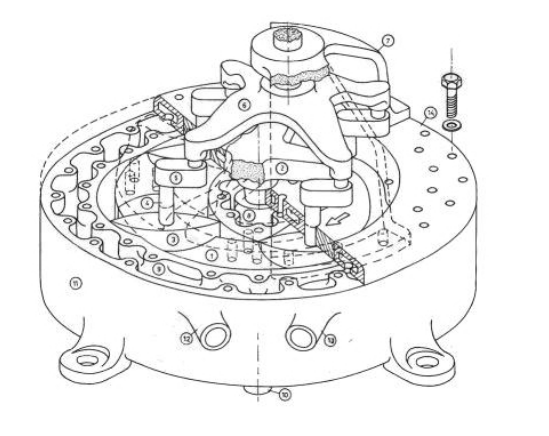
\includegraphics[width=0.5\textwidth]{perspectiva_mrcvc.png}
    \caption{Motor Rotativo de Combustión a Volumen Constante}\label{fig:mrcvc}
\end{figure}

En trabajos anteriores~\parencite{lopez13,lopez16,toth00}~se han mencionado
las características que hacen al MRCVC un motor atractivo: la geometría de la
cámara de combustión y del conjunto rotante permiten que gran parte del proceso
de combustión se realice a volumen constante, además de tener un balanceo
mecánico de fuerzas que le permite alcanzar altas velocidades de rotación.
%
Esto promete un funcionamiento más suave del motor, además de una reducción del
ruido y desgaste en comparación a motores rotativos tradicionales (Wankel) y
reciprocantes.
%
Por otro lado, hay que mencionar que los motores rotativos traen consigo una
serie de problemas como la necesidad de introducir aceite a la cámara de
combustión para lubricar elementos móviles, el solape de cámaras durante la
apertura de los puertos y, en particular al MRCVC, un complejo sistema de
sellos~\parencite{roldan20}.

%%%%%%%%%%%%%%%%%%%%%%%%%%%%%%%%%%%%%%%%%%%%%%%%%%%

La motivación de este trabajo surge del deseo de continuar con el desarrollo del
MRCVC y mejorar el pre-diseño de los sistemas de intercambio de gases, sentando
la base para una futura optimización de los mismos en un motor con requisitos de
diseño concretos.


Se buscó obtener un pre-diseño satisfactorio del sistema poniendo énfasis en la
geometría de los puertos de admisión y escape, definiendo las métricas a
utilizar para medir la eficiencia del sistema y poder realizar comparaciones
cuantitativas de los diseños propuestos.
%
Debido al costo computacional de las simulaciones necesarias para realizar esta
optimización se restringe el modelado de la geometría a las definiciones de las
posiciones de los puertos en el estator, largos y diámetros de los conductos.
%
No se repara en detalles como la forma de la transición entre las paredes del
puerto hacia la cámara, el ángulo al estator o detalles similares.

%%%%%%%%%%%%%%%%%%%%%%%%%%%%%%%%%%%%%%%%%%%%%%%%%%%
Se utilizó una serie de herramientas de simulación para la optimización, algunas
de las cuales fueron:

\begin{enumerate}
        %
    \item ICESym~\parencite{icesym}, simulador de motores de combustión interna basado en modelos cero-/uni-dimensionales (0D/1D).
        %
    \item OpenFOAM~\parencite{openfoam}, una herramienta libre de CFD (\textit{Computational Fluid Dynamics}).
        %
    \item Salome~\parencite{salome}, plataforma libre para simulación numérica.
        %
\end{enumerate}

\nomenclature[F]{\(CFD\)}{\textit{Computational Fluid Dynamics.}}

Se desarrolló un optimizador capaz de generar y evaluar diferentes geometrías
con el fin de buscar una combinación de parámetros que maximicen indicadores de
eficiencia del sistema, como por ejemplo, el rendimiento volumétrico del motor
para un rango de velocidades determinado.

El proceso de optimización consta de una primera aproximación utilizando como
punto de partida los resultados de trabajos anteriores~\parencite{lopez13}, en
los cuales se evaluó el funcionamiento de los parámetros que definen la
geometría de los sistemas de intercambio de gases, analizándose en particular:
diámetros y longitudes de conductos y reglaje o posición angular de los puertos.

La optimización se realiza con un algoritmo evolutivo (o genético) funcionando
en conjunto con ICESym, el cual provee el puntaje a cada configuración del
motor necesario para estos procesos de optimización.
%
El puntaje se introduce en la función objetivo, la cual evalúa a cada uno de los
candidatos generados por el algoritmo.

El diseño preliminar de la primera ronda de optimización se volcó en un modelo
tridimensional (3D) de los puertos, parametrizado de modo tal que se puede
alterar rápidamente la geometría, modificando variables como el diámetro de los
conductos y la posición relativa en la periferia del motor.
%
Este modelo 3D se utilizó para extraer la geometría a simular con OpenFOAM y
realizar flujometrías de las que se obtiene un valor del flujo másico
($\dot{m}$) en estado estacionario para un punto operativo del motor, es decir,
para una combinación de diferencia de presión entre puerto y cámara
($\Delta P$) y el grado de apertura del puerto ($l_{v}$).
%
El flujo másico se utilizó para medir la eficiencia con la cual escurre el gas a
través del puerto, con el objetivo de crear un mapa del coeficiente de descarga
($C_{D}$) que sea función de las variables mencionadas.
%
Este mapa se utiliza como retroalimentación del simulador de motores ICESym,
para tener un mejor modelado del flujo de gas a través de los puertos en un
rango operativo del motor y con esto realizar una nueva corrida de optimización
a fin de refinar el diseño obtenido en la primera iteración.
%
\nomenclature[PO]{\(\dot{m}\)}{Caudal másico}
\nomenclature[F]{\(C_{D}\)}{Coeficiente de descarga}

% Primer capitulo
%
A continuación se describe la organización del presente trabajo.
%
% Segundo capitulo
%
En el segundo capítulo se presenta una breve descripción del funcionamiento de
los motores de combustión interna, seguido de los indicadores utilizados para
medir el rendimiento de motores en general e indicadores particulares de la
eficiencia de los sistemas de intercambio de gases, como el rendimiento
volumétrico y la fracción de gases residuales.
%
Luego, se describe el funcionamiento del MRCVC, indicando los aspectos
sobresalientes de este motor, además de desventajas del mismo y las posibles
aplicaciones.
%
También se describe el proceso de intercambio de gases y se define el
coeficiente de descarga $C_{D}$, junto con las ecuaciones asociadas.
%
% Tercer capitulo
%
En el tercer capítulo se describen las herramientas computacionales utilizadas
en este trabajo.
%
Se presenta el simulador de motores ICESym, el optimizador desarrollado y
la integración entre ambos programas.
%
Se incluye una descripción del funcionamiento del optimizador, los motivos de
seleccionar un algoritmo de tipo evolutivo o genético, las ventajas y
desventajas, los componentes básicos y finalmente la implementación del mismo.
%
En este capítulo también se presenta el software utilizado para realizar las
flujometrías, OpenFOAM, la implementación de las condiciones iniciales y
de contorno, extracción de datos de ICESym y otras herramientas necesarias para
generar el modelo de CAD del puerto, malla y otros detalles relativos al proceso
de utilizar el programa.

% Cuarto capítulo
%
En el cuarto capítulo se presentan detalles particulares de las simulaciones
realizadas, incluyendo la geometría del motor utilizado y su implementación en
ICESym.
%
Además, se detallan la configuración de las flujometrías virtuales realizadas
con OpenFOAM, condiciones iniciales, configuración de la herramienta, esquemas
de discretización y otros parámetros importantes relacionados a las
flujometrías.
%
% Quinto capítulo
%
En el quinto capítulo se presentan los resultados del trabajo para cada una de
las etapas correspondientes.
%
% Sexto capítulo
%
Por último, se exponen las conclusiones del trabajo, opiniones finales y una
perspectiva a futuro de posibles trabajos a seguir.
 \pagebreak

\chapter{MARCO TEÓRICO}\label{capitulo:MARCO_TEORICO}
\section{Motores de Combustión Interna}

Los motores de combustión interna dieron un impulso a la actividad humana desde
los años 1860, cuando su uso comercial comenzó a popularizarse.
%
La función de estos dispositivos es la de convertir energía química del fluido
de trabajo (una mezcla de aire-combustible) en trabajo mecánico por medio de un
proceso de combustión controlada dentro del cilindro o cámara de combustión.
%
Los primeros ejemplares comerciales eran voluminosos, costosos, altamente
ineficientes y de baja potencia, con valores de rendimiento cercano al 5\% y
potencias de hasta 6 HP.

\begin{figure}[h!]
  \centering
  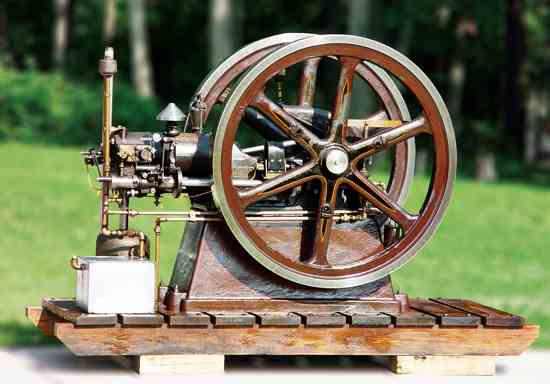
\includegraphics[width=.5\textwidth]{otto_1909.jpg}
  \caption{Motor 1909 5HP Otto Special Electric Lighting de Wayne Grenning}\label{fig:otto1909}
  % https://www.gasenginemagazine.com/gas-engines/1909-5-hp-otto-special-electric/
\end{figure}


Un paso importante hacia los motores actuales fue el desarrollo del ciclo Otto,
propuesto por Nicolaus A. Otto y Eugen Langen, cuyo primer prototipo se puso en
marcha en el año 1876.
%
Otto propuso un motor alternativo con cuatro carreras de pistón: admisión,
compresión, expansión y escape; este prototipo lograba la misma potencia con
mayor eficiencia que los motores de la época con menos de la mitad del peso y
volumen.
%
En la Figura~\ref{fig:otto1909} se ve un motor de ciclo Otto fabricado por
\emph{Otto Gas Engines Works} en el año 1909 en Filadelfia-EEUU.
%
Según la revista \emph{Gas Engine
Magazine}\footnote{\url{https://www.gasenginemagazine.com/gas-engines/1909-5-hp-otto-special-electric/}}
\footnote{ \url{https://www.youtube.com/watch?v=LPSWfg0Y3Hs} } \footnote{
\url{https://www.youtube.com/watch?v=0d0WZ0H56_U} } este motor funcionaba
directamente acoplado a una bomba \emph{TRIPLEX} de agua, como parte de un
sistema de irrigación de un club de campo de Delaware.
%
Los motores han continuado su desarrollo desde entonces, mejorando materiales,
combustibles y procesos de manufactura entre otros aspectos.
%
En las últimas décadas se ha hecho foco en disminuir el consumo de combustible,
nivel de ruido, costo de manufactura, tamaño y las emisiones de gases
contaminantes y de efecto invernadero como las de $CO_2$, $CO$ y $NO_x$, entre
otras.


El ciclo operativo de cuatro tiempos de Otto se puede expresar en términos de
carreras del pistón (véase la Figura~\ref{fig:4tiempos}), en la que se pueden
identificar dos posiciones de interés: el punto muerto superior (PMS) y el punto
muerto inferior (PMI).
%
En el PMS se tiene el volumen mínimo atrapado del cilindro y el pistón está al
final de la carrera, en el punto más alejado del eje del cigüeñal.
%
El PMI es el punto en el que se tiene el volumen máximo del cilindro y el pistón
está en el punto más cercano al eje del cigüeñal, como se ve en la
Figura~\ref{fig:pms_pmi}.
%
Las carreras de pistón del ciclo Otto son:
%
\begin{description}
%
    \item [Carrera de admisión] el pistón se mueve desde el PMS hasta el PMI con
        la válvula de admisión abierta y la de escape cerrada.
        %
        Esto provoca que ingrese una masa de aire o aire-combustible al cilindro.
%
    \item [Carrera de compresión] el pistón se mueve desde el PMI hacia el PMS
        con la válvula de admisión y escape cerradas.
        %
        Esta reducción del volumen comprime y calienta los gases en el interior
del cilindro.
        %
        En una posición angular del ciclo denominada \emph{avance de encendido}
se enciende la mezcla y comienza la combustión.
%
    \item [Carrera de expansión] la combustión produce un gran
aumento de presión y temperatura en el cilindro, la carrera de expansión parte
del PMS hacia el PMI, aprovechando la expansión en volumen de los productos de
la combustión que producen trabajo sobre la cabeza del pistón.
%
    \item [Carrera de escape o barrido] luego de la carrera de expansión, en PMI
se abre la válvula de escape y se produce el  barrido de los gases quemados,
reiniciando el ciclo.
%
\end{description}

\begin{figure}[h!]
  \centering
  \begin{subfigure}{0.6\textwidth}
    \centering
    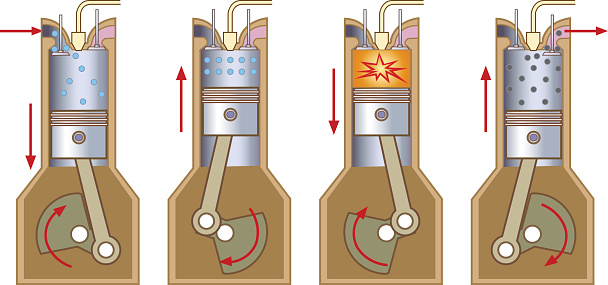
\includegraphics[width=\textwidth]{4stroke.jpg}
    \caption{Ciclo de cuatro tiempos}\label{fig:4tiempos}
  \end{subfigure}%
  \hfill
  \begin{subfigure}{0.4\textwidth}
    \centering
    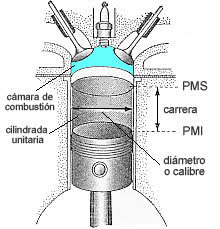
\includegraphics[width=\textwidth]{pms_pmi.jpg}
    \caption{PMS y PMI}\label{fig:pms_pmi}
  \end{subfigure}
  \caption{Ciclo de cuatro tiempos y PMS/PMI}
  \label{fig:4tiempos_pms_pmi} % Etiqueta global para la figura completa
\end{figure}

% https://www.istockphoto.com/es/vector/motor-di%C3%A9sel-de-cuatro-tiempos-gm586705100-100702521

\section{Motores Rotativos}
%
Los motores rotativos son una variante al diseño de los motores alternativos.
%
Su compacidad, balanceo y mayores velocidades de giro los vuelven más atractivos
en aplicaciones en las cuales el volumen es restringido.
%
La mayor velocidad de giro permite alcanzar mayores potencias, por lo que tienen
una menor relación peso/potencia que motores reciprocantes de potencia similar.
%
El diseño rotativo más conocido es el Wankel, cuyo primer prototipo funcional se
desarrolló cerca del año 1957.
%
Existen otros desarrollos de este tipo de motores como el motor rotativo de
pistón líquido, con un ciclo de combustión a volumen constante denominado
HECH~\parencite{hehc_05} y el objeto de este trabajo, el Motor Rotativo de
Combustión a Volumen Constante (MRCVC).

Si bien estos motores son una alternativa interesante a los motores
reciprocantes, la geometría y aspectos constructivos implican que en algunos
casos es necesario introducir aceite mezclado con el lubricante en la cámara de
combustión para lubricar las partes móviles.
%
% Además tienen una mayor superficie de transferencia de calor causando una mayor
% pérdida de calor en comparación con los motores reciprocantes.
%
En la actualidad, los requisitos de niveles de emisiones ambientales de ciertos
gases hacen estos motores inviables para el uso comercial masivo, sin embargo la
compacidad del motor los vuelve atractivos en aplicaciones militares como por
ejemplo para vehículos aéreos no tripulados.

%%%%%%%%%%%%%%%%%%%%%%%%%%%%%%%%%%%%%%%%%%%%%%%%%%%%%%%%%%%%%%%%%%%%%%%%%%%%%%%


\section{Parámetros Operativos e Indicadores de Rendimiento}
%
Para poder comparar entre diferentes diseños de motores se deben conocer algunos
parámetros operativos e indicadores de rendimiento.
%
Algunas de las características más importantes de un motor son:
%
\begin{enumerate}
        %
    \item Potencia y torque
        %
    \item Rango de velocidades de operación
        %
    \item Consumo y costo de combustible
        %
    \item Costo inicial, de operación y de mantenimiento
        %
    \item Confiabilidad
        %
    \item Niveles de ruido y emisiones contaminantes
        %
\end{enumerate}

Estas características se pueden expresar de manera más genérica en función de la
potencia, geometría u otros aspectos de un motor para obtener valores que se
pueden comparar directamente entre motores.
%
Por ejemplo, al cociente entre el trabajo entregado por ciclo y la cilindrada
de un motor se lo conoce como presión media efectiva o \emph{mep}, por sus
siglas en inglés.
%
Algunos parámetros operativos e indicadores se describen en las secciones
siguientes.

%%%%%%%%%%%%%%%%%%%%%%%%%%%%%%%%%%%%%%%%%%%%%%%%%%%%%%%%%%%%%%%%%%%%%%%%%%%%%%%

\subsection{Volumen Desplazado}
%
El volumen desplazado se define como la diferencia entre el volumen máximo
($V_{max}$) y mínimo ($V_{min}$) que ocupa la cámara de combustión:

\begin{equation}\label{eq:vol_desp} V_d = V_{max}-V_{min}
\end{equation}
%
\nomenclature[PO]{\(V\)}{Volumen}
\nomenclature[G]{\(V_d\)}{Volumen desplazado}
% \nomenclature[G]{\(V_{min}\)}{Volumen mínimo en la cámara de combustión}
\nomenclature[G]{\(V_{max}\)}{Volumen máximo de la cámara}

%%%%%%%%%%%%%%%%%%%%%%%%%%%%%%%%%%%%%%%%%%%%%%%%%%%%%%%%%%%%%%%%%%%%%%%%%%%%%%%

\subsection{Relación de Compresión}

Se define como el cociente entre el volumen máximo y el volumen mínimo del ciclo:
%
\begin{equation}\label{eq:rel_comp}
  r_c = \frac{V_{max}}{V_{min}} = \frac{V_d+V_{min}}{V_{min}}
\end{equation}

\nomenclature[G]{\(V_{min}\)}{Volumen mínimo de la cámara}
\nomenclature[PO]{\(r_c\)}{Relación de compresión}
%
Es uno de los parámetros más importantes de un motor ya que afecta a la presión
máxima que se puede obtener en la cámara de combustión, la \emph{performance},
la potencia entregada, los esfuerzos mecánicos y el rendimiento del motor.

%%%%%%%%%%%%%%%%%%%%%%%%%%%%%%%%%%%%%%%%%%%%%%%%%%%%%%%%%%%%%%%%%%%%%%%%%%%%%%%

\subsection{Trabajo Indicado por Ciclo}
%
El trabajo entregado por el gas dentro del cilindro al pistón por cada ciclo de
operación se denomina trabajo indicado por ciclo y se obtiene al integrar la
presión en función del volumen a lo largo de todo el ciclo:

\begin{equation}\label{eq:w_indicado}
  W_{c,i} = \oint p dV
\end{equation}
\nomenclature[PO]{\(W_{c,i}\)}{Trabajo indicado por ciclo}

Para motores de 4 tiempos se debe diferenciar entre trabajo bruto y trabajo neto.
%
En el último se tiene en cuenta el trabajo de bombeo que resulta de la
diferencia del trabajo realizado durante las carreras de admisión y escape, por
lo que este indicador se puede diferenciar en:
%
\begin{description}
  \item [Trabajo indicado bruto por ciclo] $W_{c,ig}$, mide el trabajo realizado
por el motor en las carreras de compresión y expansión.
\nomenclature[PO]{\(W_{c,ig}\)}{Trabajo indicado bruto por ciclo}
        %
  \item [Trabajo indicado neto por ciclo] $W_{c,in}$, mide el trabajo realizado
por el motor considerando las 4 carreras del ciclo.
\nomenclature[PO]{\(W_{c,in}\)}{Trabajo indicado neto por ciclo}
        %
  \item [Trabajo de bombeo] es la diferencia entre el trabajo bruto y neto, y
mide el trabajo realizado durante los procesos de admisión y escape.
  \item [Trabajo de fricción mecánica] es el trabajo consumido por el rozamiento
entre partes móviles del motor.
        %
\end{description}

%%%%%%%%%%%%%%%%%%%%%%%%%%%%%%%%%%%%%%%%%%%%%%%%%%%%%%%%%%%%%%%%%%%%%%%%%%%%%%%

\subsection{Consumo Específico de Combustible y Rendimiento de Conversión del
Combustible}
%
El consumo específico de combustible, \emph{sfc} por sus siglas en inglés, se
define como el cociente entre el caudal másico de combustible ($\dot{m_f}$)
consumido por unidad de potencia $P$ entregada por el motor:
\nomenclature[PO]{\(\dot{m_f}\)}{Caudal másico de combustible}

\begin{equation}\label{eq:sfc} sfc = \frac{\dot{m_f}}{P}
\end{equation}
\nomenclature[PO]{\(sfc\)}{Consumo específico de combustible}

Este parámetro mide la eficiencia con la que el motor utiliza el combustible
para una condición de operación dada.
%
En motores de encendido por chispa se tienen valores típicos de alrededor de
$235\text{g/(kW}\cdot h$~\parencite{heywood}.

Una versión similar de este indicador adimensionalizado en relación a la energía
suministrada por el combustible, es el \emph{rendimiento de conversión del
combustible} $\eta_f$, que se relaciona al \emph{sfc} por medio del poder
calorífico del combustible, $Q_{HV}$.

\nomenclature[PO]{\(Q_{HV}\)}{Poder calorífico}
\nomenclature[PO]{\(\eta_f\)}{Rendimiento de conversión de combustible}

\begin{equation}\label{eq:eta_f} \eta_f = \frac{1}{sfc \cdot Q_{HV}}
\end{equation}

El valor de $Q_{HV}$ es una propiedad del combustible que se determina en un
ensayo de laboratorio.
%
Valores típicos para los combustibles comerciales basados en hidrocarburos son
de 42 a 44 $MJ/kg$.

%%%%%%%%%%%%%%%%%%%%%%%%%%%%%%%%%%%%%%%%%%%%%%%%%%%%%%%%%%%%%%%%%%%%%%%%%%%%%%%

\subsection{Presión Media Efectiva}
%
La presión media efectiva o $mep$ es un indicador cuya variación es proporcional
al torque del motor.
%
El trabajo realizado por ciclo se puede calcular como
$W_c = \frac{P \cdot n_R}{N}$, donde $n_R$ es el número de revoluciones del
cigüeñal por cada ciclo y $N$ son las revoluciones por segundo del eje del motor.
%
Para motores de cuatro tiempos $n_R=2$, y $n_R=1$ para motores de dos tiempos.
%
De este modo, la presión media efectiva se define como:

\begin{equation}\label{eq:mep}
  mep = \frac{W_{c}}{V_d} = \frac{P \cdot n_R}{V_d \cdot N}
\end{equation}
%

Se puede diferenciar entre presión media efectiva indicada (\emph{imep}), al
freno (\emph{bmep}) y de fricción (\emph{fmep}), utilizando el valor de potencia
correspondiente en la ecuación (\ref{eq:mep}).
%
El valor de \emph{mep} (al igual que el torque) de un motor varía con la
velocidad de operación, siguiendo de cerca las tendencias de la curva de
rendimiento volumétrico como se puede ver en el ejemplo de la
Figura~\ref{fig:bmep_tipica}.

En la actualidad, valores típicos de \emph{bmep} de motores de encendido por
chispa (SI por sus siglas en inglés) naturalmente aspirados rondan los 1050 kPa
a 1250 kPa para la velocidad a la que se alcanza el torque máximo~\parencite{heywood}.

\begin{figure}[h!]
  \centering
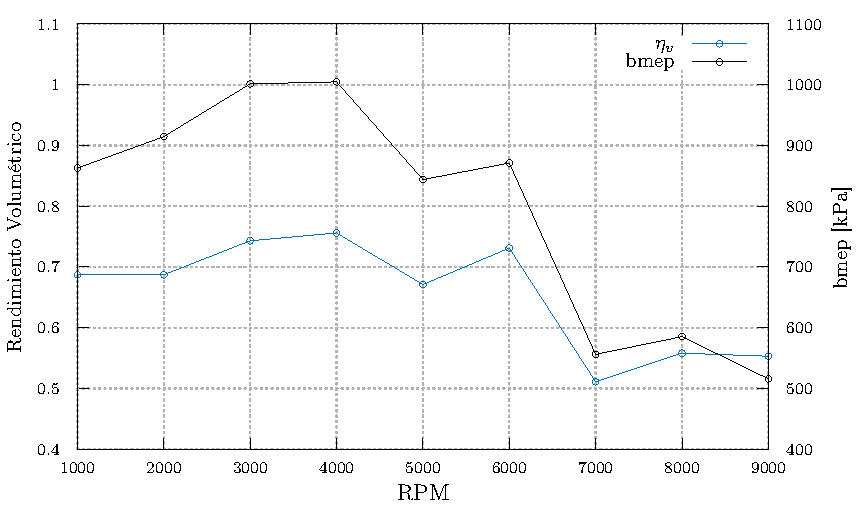
\includegraphics[width=\textwidth]{./gnuplot/bmep_vs_rendVol.pdf}
    \caption{\emph{bmep} y rendimiento volumétrico vs velocidad de operación.}
    \label{fig:bmep_tipica}
\end{figure}

\nomenclature[PO]{\(n_R\)}{Revoluciones de cigüeñal por ciclo}
\nomenclature[PO]{\(N\)}{Velocidad de giro del motor}
\nomenclature[PO]{\(bmep\)}{Presión media efectiva bruta}
\nomenclature[PO]{\(imep\)}{Presión media efectiva indicada}
\nomenclature[PO]{\(mep\)}{Presión media efectiva (\textit{mean effective pressure})}

%%%%%%%%%%%%%%%%%%%%%%%%%%%%%%%%%%%%%%%%%%%%%%%%%%%%%%%%%%%%%%%%%%%%%%%%%%%%%%%

\subsection{Rendimiento Volumétrico}
%
El rendimiento volumétrico mide la eficiencia del sistema de admisión.
%
Es la relación entre el volumen de aire realmente introducido al cilindro y el
volumen teórico que debería entrar al cilindro si este estuviera completamente
lleno con aire a la densidad del ingreso al sistema de admisión ($\rho_{a,i}$).
%
En términos concretos se define como el cociente entre el caudal másico de aire
que ingresa al sistema de admisión ($\dot{m}_{a}$) y la velocidad con la que el
volumen es desplazado por el pistón.
%
En otras palabras, este indicador mide la eficiencia con la que el motor bombea
aire.
\nomenclature[PO]{\(\dot{m}_{a}\)}{Caudal másico de aire}

\begin{equation}\label{eq:eta_v}
  \eta_v = \frac{2\dot{m_a}}{\rho_{a,i}V_d N}
\end{equation}

\nomenclature[PO]{\(\rho_{a,i}\)}{Densidad del aire de admisión}
\nomenclature[PO]{\(m_{a,i}\)}{Masa de aire inductada}

Una forma alternativa a la ecuación anterior es considerando la masa total de aire que
ingresa al cilindro por ciclo, ($m_{a}$):

\begin{equation}\label{eq:eta_v_alt}
  \eta_v = \frac{m_a}{\rho_{a,i}V_d}
\end{equation}

Para motores naturalmente aspirados la densidad del aire de admisión
$\rho_{a,i}$ se toma comúnmente como la densidad atmosférica, por lo que en ese
caso $\eta_v$ mide el rendimiento de todo el sistema de admisión.
%
\nomenclature[PO]{\(\rho_a\)}{Densidad del aire}
\nomenclature[PO]{\(\eta_v\)}{Rendimiento volumétrico}

El valor del rendimiento volumétrico máximo típico para motores naturalmente
aspirados ronda el 90\%~\parencite{heywood}.
%
Su valor se ve afectado por varios fenómenos siendo los más importantes:

\begin{description}
        %
    \item [Efectos cuasiestáticos] Combustible, relación aire/combustible,
vaporización del combustible en el conducto de admisión, temperatura del aire de
admisión, relación entre presión de admisión y escape, relación de compresión,
etc.
  \item [Pérdidas de carga por fricción viscosa] Las pérdidas viscosas aumentan
con la velocidad de flujo y aumentan a medida que aumenta la velocidad de giro
del motor.
        %
Además, se tienen las pérdidas por la presencia de filtros , puertos, válvulas
que generan pérdidas localizadas.
        %
  \item [Transferencia de calor en el sistema de admisión] La mezcla se calienta
por transferencia de calor y esto disminuye la densidad de la misma, reduciendo
la masa de aire.
        %
  \item [Reglaje de las válvulas/puertos] El punto de apertura y cierre de las
válvulas o  puertos (reglaje) es clave para el funcionamiento del motor.
        %
Dependiendo del reglaje que se elija, se puede favorecer el flujo a determinada
velocidad de operación.
        %
    \item [Efecto ram] A grandes velocidades de flujo la inercia del gas al
momento del cierre de la válvula (o puerto) de admisión permite un mayor ingreso
de masa fresca al cilindro.
        %
    \item [Flujo bloqueado en puertos de admisión] En las zonas de
menor área de pasaje la velocidad del fluido puede aumentar hasta alcanzar la
velocidad del sonido, lo cual se conoce como bloqueo y limita el caudal másico que
puede ingresar a la cámara de combustión.
        %
        %
    \item [Sintonía de admisión y escape] El diseño de los sistemas de
admisión y escape puede favorecer el funcionamiento de los mismos a determinada
velocidad de operación, lo cual se logra aprovechando las ondas de presión que
se producen por la apertura y cierre de las válvulas o puertos.
      %
Véanse las secciones~\ref{cap2_sec_sintonia_admision} y~\ref{cap2_sec_sintonia_escape}.
        %
  \item [Sobrecarga] Por medio de un compresor o turbocompresor se puede
aumentar la presión en el sistema de admisión forzando más aire a la cámara de
combustión.
        %
\end{description}

La curva de rendimiento volumétrico es muy similar a la curva de torque o de
presión media efectiva (ver Figura~\ref{fig:bmep_tipica}).
%
La cantidad de aire que ingresa al motor está directamente relacionada con el
trabajo que puede realizar por ciclo de operación.
%
Este indicador es central en la evaluación del desempeño de los sistemas de
intercambio de gases y por este motivo es el principal indicador utilizado en
este trabajo.
%
Se buscó que la curva de rendimiento volumétrico de los motores simulados tenga
un máximo para velocidades cercanas o mayores a 6000 RPM aprovechando el
balanceo mecánico del motor, que permite funcionar y seguir entregando potencia
a altas RPM.
%
La curva debe ser preferentemente suave para todo el régimen de funcionamiento
del motor.
%
Estos y otros efectos se describen en detalle en la
literatura~\parencite{heywood}.
%

Con respecto a la mezcla aire-combustible, se define la relación
de equivalencia $\phi$ a partir del cociente de relaciones combustible/aire (F/A)
de la mezcla y combustible/aire estequiométrica como se indica en la
ecuación~(\ref{eq:phi}).
%
Para más detalles en cuanto a la composición estequiométrica ver la ecuación
~(\ref{eq:estequeometrica}).

\begin{equation}
  \label{eq:phi}
  \phi = \frac{(F/A)_{mezcla}}{(F/A)_{estequiométrica}}
\end{equation}

En estos términos una mezcla pobre en combustible tiene $\phi < 1$, una mezcla
estequiométrica $\phi=1$ y una mezcla rica en combustible $\phi > 1$.


\subsection{Fracción de Gases Residuales}
%
Al final del proceso de barrido, con la válvula de escape cerrada,
pueden quedar gases residuales de la combustión atrapados en el cilindro.
%
Estos gases permanecen para el próximo ciclo de trabajo, afectando el
rendimiento volumétrico, el trabajo obtenido, la eficiencia y las emisiones.
%
La fracción de gases residuales se define como el cociente entre la masa de
gases quemados en el cilindro  al inicio de la fase cerrada del ciclo ($m_{r}$)
y la masa total atrapada en el cilindro ($m$):


\begin{equation}
    x_{r} = \frac{m_{r}}{m}
\end{equation}

\nomenclature[PO]{\(x_{r}\)}{Fracción de gases residuales}
\nomenclature[PO]{\(m_{r}\)}{Masa residual en la cámara de combustión}
\nomenclature[PO]{\(m\)}{Masa total en la cámara de combustión}

En el MRCVC existe un fenómeno llamado solape de cámaras~\parencite{lopez13}.
%
Durante el proceso de admisión de gases frescos, una cámara puede verse afectada
por la apertura del puerto de admisión de la cámara siguiente, que se encuentra
a mayor presión y temperatura debido a que está finalizando el proceso de escape
y comenzando el de admisión, pudiendo provocar un aumento de la cantidad de gases
residuales.


La presencia de gases residuales en la cámara tiene varios efectos en la
combustión y el rendimiento del motor.
%
Algunos pueden ser beneficiosos como la reducción de emisiones nocivas y la
reducción del consumo de combustible.
%
Por otro lado puede tener efectos negativos como la reducción del rendimiento
volumétrico.
%
\begin{description}
        %
  \item[Dilución de la mezcla] el gas residual ocupa volumen que no puede ocupar la mezcla fresca.
        %
  \item[Temperatura] los gases residuales están a mayor temperatura y al mezclarse con la mezcla fresca aumenta su temperatura y volumen, reduciendo la cantidad de mezcla fresca que puede ingresar a la cámara.
        %
  \item[Reducción de $NO_{x}$] un efecto beneficioso es la reducción de emisiones de óxidos de nitrógeno.
        %
  \item[EGR] en algunos motores modernos se recirculan gases quemados (\textit{Exhaust Gas Recycle}) para reducir emisiones de $NO_{x}$ y controlar el consumo de combustible. En motores SI se puede utilizar hasta un 30\% de EGR, estos valores son aún mayores para motores de encendido por compresión~\parencite{heywood}.
        %
  \item[Rendimiento volumétrico] la presencia de gases residuales en la cámara disminuye el volumen que puede ocupar la mezcla fresca, lo cual tiene un impacto negativo en el rendimiento volumétrico.
        %
\end{description}

%%%%%%%%%%%%%%%%%%%%%%%%%%%%%%%%%%%%%%%%%%%%%%%%%%%%%%%%%%%%%%%%%%%%%%%%%%%%%%%
\section{Sintonización del Sistema de Admisión}\label{cap2_sec_sintonia_admision}
%
En motores naturalmente aspirados, la apertura de la válvula o puerto de
admisión produce una onda de depresión que viaja desde el puerto de admisión
hacia el extremo opuesto del conducto de admisión.
%
Cuando esta onda de presión llega al pleno de admisión, se refleja como una
onda de sobrepresión que toma un tiempo $t$ en alcanzar nuevamente el puerto.
%
Si el tiempo que toma la onda en reflejarse es tal que alcanza el puerto justo
antes del cierre de la válvula, el sistema está sintonizado.
%
Esta sobrepresión permite que ingrese una mayor cantidad de masa fresca al
cilindro, aumentando la cantidad de trabajo que se puede realizar.

En la Figuras~\ref{fig:sintonia_heywood} se muestran las curvas de presión en
función del ángulo de cigüeñal para un motor operando a $1200$ y $4800$ RPM, en
donde se indican los períodos en los que se encuentran abiertas las válvulas de
admisión (IO) y de escape (EO).
%
Los valores $p_{1}$, $p_{2}$ y $p_{3}$ hacen referencia a diferentes posiciones
a lo largo de los conductos de admisión y escape.
%
Se puede ver que para $p_{1}$ a $4800$ RPM hay un claro pico de presión justo al
cierre del puerto de admisión, el sistema está sintonizado para esta velocidad.

Debido a que la onda de presión debe viajar dos veces la longitud del conducto
de admisión desde el momento que abre el puerto de admisión, para sintonizar el
sistema a bajas velocidades, se requieren longitudes mayores, lo que hace más
grande el sistema de admisión.
%
La sintonía a mayores velocidades de admisión es preferida, porque usualmente se
tiene el máximo de torque y de potencia a mayores RPM, además reduce la
necesidad de conductos más largos.
%
En motores multi-cilíndricos se utiliza un pleno de admisión.
%
Este dispositivo proporciona un volumen grande de aire que sirve el propósito de
cámara de resonancia (resonador de Helmholtz).
%
Se puede ajustar la resonancia de modo que las oscilaciones de presión internas
produzcan una sobrepresión en el múltiple de admisión que puede aprovecharse
para incrementar el llenado del cilindro cuando el pistón promedia la carrera de
admisión.

\begin{figure}[h!]
  \centering
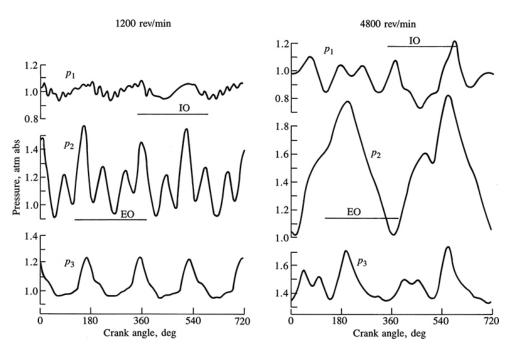
\includegraphics[width=0.8\textwidth]{sintonia_heywood.jpg}
    \caption{Diagrama de presión vs ángulo de cigüeñal~\parencite{heywood}}\label{fig:sintonia_heywood}
\end{figure}

%%%%%%%%%%%%%%%%%%%%%%%%%%%%%%%%%%%%%%%%%%%%%%%%%%%%%%%%%%%%%%%%%%%%%%%%%%%%%%%
\section{Sintonización del Sistema de Escape}\label{cap2_sec_sintonia_escape}

De forma análoga al sistema de admisión, al momento de la apertura del puerto o
válvula de escape los gases quemados se encuentran a  mayor presión que el gas
en el conducto.
%
Esto crea una onda de sobrepresión que viaja por el escape hasta alcanzar el
final del mismo o un área de gran volumen, como el catalizador o el silenciador.
%
Desde esta zona se refleja como una onda de depresión, que en caso de alcanzar
el puerto en los instantes previos al cierre de la válvula, ayuda a evacuar una
mayor cantidad de gas, disminuyendo la fracción de gases residuales.

En la Figura~\ref{fig:sintonia_heywood} se ve que para el escape en $p_2$ se
tiene una depresión justo al cierre del puerto, este sistema está sintonizado
para 4800 RPM.
%
Es notorio el contraste con el mismo puerto a 1200 RPM, en donde se ve un pico de
presión cerca del cierre del puerto.
%
%%%%%%%%%%%%%%%%%%%%%%%%%%%%%%%%%%%%%%%%%%%%%%%%%%%%%%%%%%%%%%%%%%%%%%%%%%%%%%%

\section{Combustión}
%
La combustión es un proceso en el que se libera la energía química del
combustible.
%
La geometría de un motor de combustión interna permite aprovechar
el aumento de presión y temperatura para convertir energía química en trabajo
mecánico.


En un motor de encendido por chispa se tiene una mezcla de aire-combustible en
la cámara de combustión.
%
Dependiendo del tipo de motor, la mezcla se puede formar en el conducto de
admisión, inyectando combustible en algún punto del sistema o se puede producir
la mezcla en la cámara por la inyección directa de combustible.
%
En un motor de encendido por compresión, la mezcla combustible se forma en la
cámara de combustión y la inyección de combustible se realiza directamente en la
cámara, cerca del PMS al final de la carrera de compresión.
%
En este caso las condiciones de presión y temperatura dentro de la cámara producen el
auto-encendido de la mezcla y el inicio del proceso de combustión.

\begin{figure}[h!]
  \centering
  \begin{subfigure}{0.3\textwidth}
    \centering
    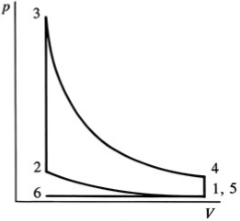
\includegraphics[width=\textwidth]{combustion_vol_cte.png}
    \caption{Volumen Constante}\label{fig:comb_vcte}
  \end{subfigure}%
  \begin{subfigure}{0.3\textwidth}
    \centering
    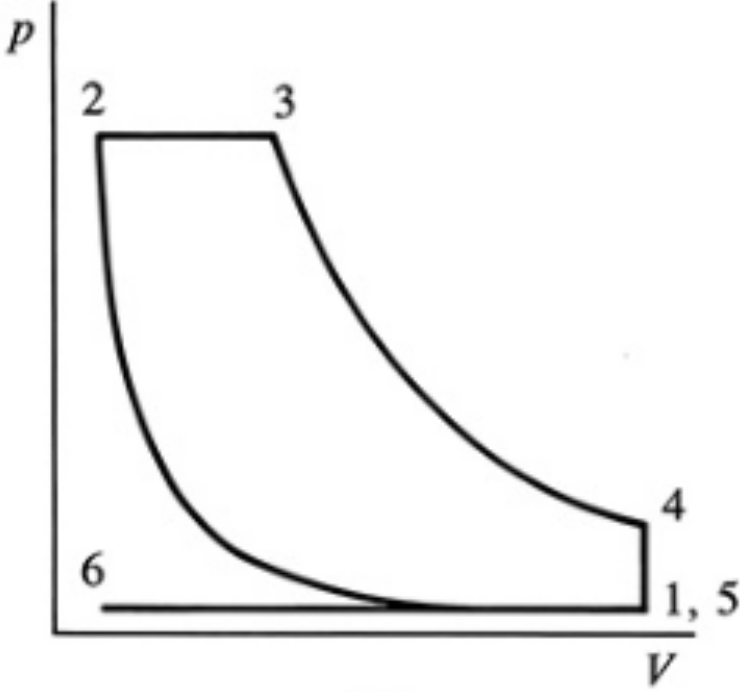
\includegraphics[width=\textwidth]{combustion_presion_cte.png}
    \caption{Presión Constante}\label{fig:comb_pcte}
  \end{subfigure}%
  \begin{subfigure}{0.3\textwidth}
    \centering
    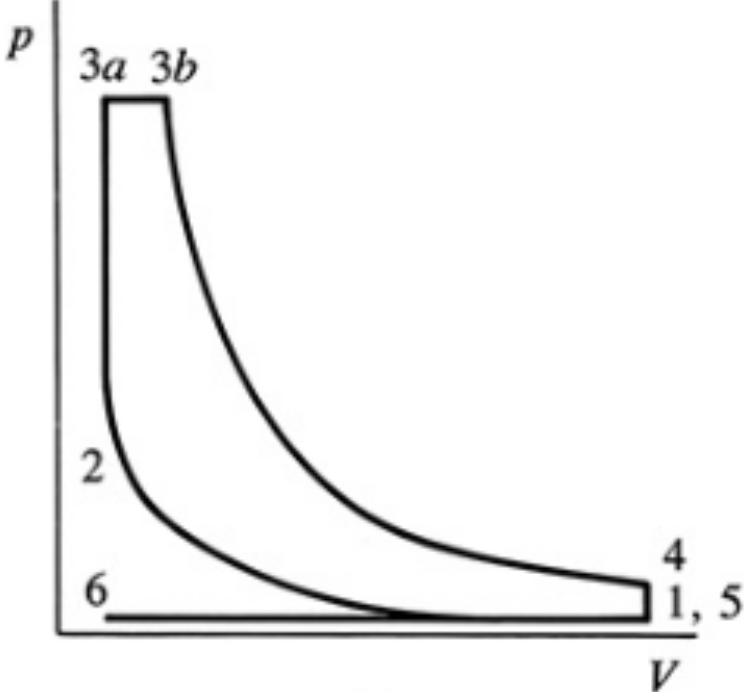
\includegraphics[width=\textwidth]{combustion_presion_limitada.png}
    \caption{Presión Limitada}\label{fig:comb_plim}
  \end{subfigure}
  \caption{Diagramas P-V para ciclos ideales\parencite{heywood}}\label{fig:ciclos_ideales}
\end{figure}

El MRCVC es un motor de combustión interna en el que, debido a su geometría,
gran parte de la combustión ocurre a volumen constante.
%
Esto se puede apreciar en la Figura~\ref{fig:mrcvc_vol_cte}, en la cual se
representa la variación del volumen en función del ángulo del cigüeñal.
%
Para visualizar el mayor rendimiento de la combustión a volumen constante  se
pueden analizar los modelos ideales de ciclos operativos~\parencite{heywood},
considerando un gas ideal con calores específicos constantes como fluido de
trabajo.
%
Se tienen tres casos de combustión: a volumen constante, presión constante o presión
limitada, obteniendo expresiones para el rendimiento de conversión del
combustible~(\ref{eq:rendimiento_p_lim}) y de $imep$ en función de la presión
mínima $p_1$~(\ref{eq:imep_p1}) y máxima $p_3$~(\ref{eq:imep_p3}) del ciclo.
%
Tanto la combustión a volumen constante como a presión constante son casos
extremos de la combustión a presión limitada, por lo que se puede utilizar el
rendimiento de conversión de combustible del ciclo de presión limitada para
comparar entre ambos extremos.

\nomenclature[F]{\(C_{V}\)}{Capacidad calorífica a volumen constante}
\nomenclature[F]{\(C_{P}\)}{Capacidad calorífica a presión constante}

\begin{align}
    \label{eq:rendimiento_p_lim}
    %
  \eta_{f,i} &= 1 - \frac{1}{r_c^{\gamma - 1}} \left[ \frac{\alpha \beta^\gamma-1}{\alpha \gamma (\beta-1)+\alpha-1} \right]\\
  \alpha &= \frac{P_3}{P_2}\\ \beta &= \frac{V_{3b}}{V_{3a}}
    %
\end{align}


\begin{equation}
    \label{eq:Q*} Q^{*}=  \frac{m_{f}Q_{LHV}}{m}
    %
\end{equation}

\nomenclature[PO]{\(Q_{LHV}\)}{Poder calorífico inferior}
\nomenclature[PO]{\(m_{f}\)}{Masa de combustible en la cámara de combustión}


\begin{equation}
    \label{eq:imep_p1} \frac{imep}{p_1} = \frac{Q^*}{c_v T_1 (\gamma-1)} \left( \frac{r_c}{r_c-1} \right) \eta_{f,i}
    %
\end{equation}

\begin{equation}
    \label{eq:imep_p3} \frac{imep}{p_3} = \frac{1}{\alpha r_c^\gamma} \left( \frac{Q^*}{c_v T_1} \right) \left(\frac{1}{\gamma-1} \right) \left( \frac{r_c}{r_c-1} \right) \eta_{f,i}
    %
\end{equation}

En el caso en que  $\alpha=1 \rightarrow P_3=P_2$ se tiene el ciclo de
combustión a presión constante, y en caso de que
$\beta=1 \rightarrow V_{3a}=V_{3b}$ se tiene el ciclo de combustión a volumen
constante (ver Figura~\ref{fig:ciclos_ideales}).

Graficando la ecuación~(\ref{eq:rendimiento_p_lim}) en función de la relación de
compresión $r_c$ (Figura~\ref{fig:rendimientos}), se observa que a igual
relación de compresión, el ciclo a volumen constante presenta mayor rendimiento
de conversión de combustible.

Del mismo modo, graficando la relación entre la presión media efectiva indicada
y la presión máxima del ciclo, $imep/p_3$, se observa que a igual relación de
compresión el ciclo de combustión a presión constante presenta mayores valores
de $imep$ en relación a la presión máxima.
%
Estso se debe a las altas presiones alcanzadas en el ciclo ideal de combustión a
volumen constante.
%
La presión máxima que se puede alcanzar en el ciclo real tiene limitaciones
relacionadas a mayores pérdidas de masa (y presión) a través de sellos y la
resistencia mecánica de los componentes del motor.
%
Además, mayores presiones están asociadas con mayores temperaturas en la cámara
de combustión.

\begin{figure}[h!]
  \centering
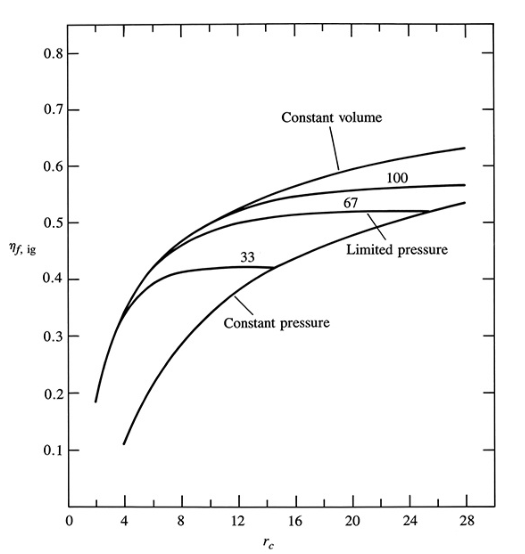
\includegraphics[width=0.6\textwidth]{ciclo/comparativa_rendimientos_ciclos.png}
    \caption{Rendimiento de conversión del combustible en función de $r_c$ para
ciclos de gas ideal de combustión a volumen constante, a presión constante y a
presión limitada~\parencite{heywood}} \label{fig:rendimientos}
    %
\end{figure}


\subsection{Propiedades Termodinámicas de Mezclas aire-combustible}\label{subsec:prop_mezcla}
%
Fue necesario estimar las propiedades termodinámicas de la mezcla para obtener
algunas variables utilizadas para calcular las condiciones iniciales del gas en
las flujometrías.
%
En lo que respecta a la simulación del ciclo del motor, ICESym contiene rutinas
computacionales para calcular el estado termodinámico del fluido de trabajo en
el ciclo operativo.
%
En este apartado se detallan las hipótesis y modelos utilizados en las rutinas
computacionales para el cálculo de las propiedades termodinámicas de las mezclas
de aire-combustible quemadas y sin quemar, para el uso en las condiciones
iniciales requeridas en las flujometrías.

En la simulación del MRCVC se utilizó una mezcla estequiométrica de
aire-isooctano.
%
La reacción estequiométrica para un hidrocarburo genérico se indica en la
ecuación~(\ref{eq:estequeometrica_generica}).

\begin{equation} \label{eq:estequeometrica_generica}
  C_{a}H_{b} + \left(a + \frac{b}{4}\right) \left(O_{2}+3,772N_{2}\right) \rightarrow a CO_{2} + \frac{b}{2} H_{2}O + 3,773 \left(a + \frac{b}{4}\right) N_{2}
\end{equation}

Las rutinas computacionales utilizadas para calcular las propiedades
termodinámicas de las mezclas aire-combustible aproximan las propiedades
químicas de cada especie en la mezcla con expresiones polinómicas.

Para cada compuesto $i$ de la mezcla a temperatura estándar $T(K)$ y 1 atmósfera
de presión se aproxima el calor específico a presión constante
$\widetilde{c_{p,i}}$ por la ecuación~(\ref{eq:cp}), la entalpía estándar
$\widetilde{h_{i}}$ por la ecuación~(\ref{eq:h}) y la entropía estándar
$\widetilde{s_{i}}$ por la ecuación~(\ref{eq:s}):

\nomenclature[PO]{\(h_{i}\)}{Entalpía estándar}
\nomenclature[PO]{\(s_{i}\)}{Entropía estándar}

\begin{equation}\label{eq:cp} \frac{\widetilde{c_{p,i}}}{T} = a_{i1} + a_{i2}T + a_{i3}T^{2} + a_{i4}T^{3} + a_{i5}T^{4}
\end{equation}

\begin{equation}\label{eq:h} \frac{\widetilde{h_{i}}}{\widetilde{R}T} = a_{i1} + \frac{a_{i2}}{2}T + \frac{a_{i3}}{3}T^{2} + \frac{a_{i4}}{4}T^{3} + \frac{a_{i5}}{5}T^{4} +\frac{a_{i6}}{T}
\end{equation}

\begin{equation}\label{eq:s} \frac{\widetilde{s_{i}}}{\widetilde{R}} = a_{i1} \ln{T} + a_{i2}T + \frac{a_{i3}}{2}T^{2} + \frac{a_{i4}}{3}T^{3} + \frac{a_{i5}}{4}T^{4} + a_{i7}
\end{equation}

\nomenclature[PO]{\(a_{i}\)}{Coeficiente de polinómicas utilizadas para cálculo de $\widetilde{c_{p}}$, $\widetilde{h}$, $\widetilde{s}$.}

La base de datos seleccionada para el aire y los productos de la combustión es
la utilizada por Chemkin~\parencite{chemkin} y los datos del isooctano fueron
tomados de~\cite{raine}.

La finalidad de estas rutinas (por fuera de las incluidas en ICESym) es la de
obtener la masa molar de la mezcla $M_{M}$, la viscosidad dinámica $\mu$, el
calor específico a presión constante $C_{P}$, la relación de calores
específicos $\gamma$ y el número de Prandtl $P_{r}$, ya que todos estos valores
son requeridos para obtener las condiciones iniciales de las flujometrías.

La masa molar de la mezcla $M_{M}$ se calcula a partir de la suma de las masas
molares $M_{i}$ y la fracción molar de cada especie química presente en la
mezcla $x_{i}$, ver ecuación~(\ref{eq:mw}).
%
La viscosidad $\mu$ de los productos de la combustión de aire e hidrocarburos
para temperaturas $T\in [500; 4000]K$, presiones $P\in[1; 100]atm$ y relaciones
de equivalencia $\phi \in [0;4]$ se puede aproximar con la
ecuación~(\ref{eq:mu}).
%
Del mismo modo, el número de Prandtl de productos de la combustión de
hidrocarburos y aire se puede estimar en función del $\gamma$ de la mezcla,
para $\phi\leq 1$ con la ecuación~(\ref{eq:pr})~\parencite{heywood}:

\nomenclature[PO]{\(x_{i}\)}{Fracción molar de una especie química ``i''}

\begin{equation}\label{eq:mw}
  M_{M} = \sum_{i} M_{i}x_{i}
\end{equation}

\begin{equation}\label{eq:mu}
  \mu_{productos} = \frac{\mu_{aire}} {1 + 0,027 \phi} = \frac{3,3\times 10^{-7} T^{0,7}} {1 + 0,027 \phi}
\end{equation}

\begin{equation}\label{eq:pr}
    \Pr = 0,05 + 4,2 (\gamma - 1) - 6,7 {(\gamma - 1)}^{2}
\end{equation}

%%%%%%%%%%%%%%%%%%%%%%%%%%%%%%%%%%%%%%%%%%%%%%%%%%%%%%%%%%%%%%%%%%%%%%%%%%%%%%%%%

\section{Coeficiente de Descarga $C_{D}$}\label{subsec:cap2_cd}
%
La pérdida de carga localizada en los puertos de admisión y escape se puede
representar a través del coeficiente de descarga, $C_{D}$.
%
Este coeficiente varía con la geometría y condiciones de operación del puerto,
siendo $C_{D}=1$ el caso ideal sin pérdida de carga localizada.
%
Es un parámetro importante porque permite obtener una mejor estimación del flujo
másico real en el puerto y se define como:

\begin{equation}
  C_{D} = \frac{\text{flujo másico real}}{\text{flujo másico ideal}}
\end{equation}

El $C_{D}$ de un puerto se puede obtener experimentalmente en un banco de prueba
mediante un ensayo que consiste en medir el caudal que circula por un puerto con
una presión de descarga fija que, en equipos comerciales varía entre $250-700$
mm.c.a.
%
Comúnmente estos ensayos se realizan en un banco que incluye solamente la tapa
de cilindros y una camisa que simula el cilindro de la cámara de combustión,
dejando de lado otros elementos del sistema como pistón, los conductos de
admisión y otros.
%
En la imagen~\ref{fig:banco_flujometrias} se muestra un banco de pruebas
comercial.

\begin{figure}[h!]
  \centering
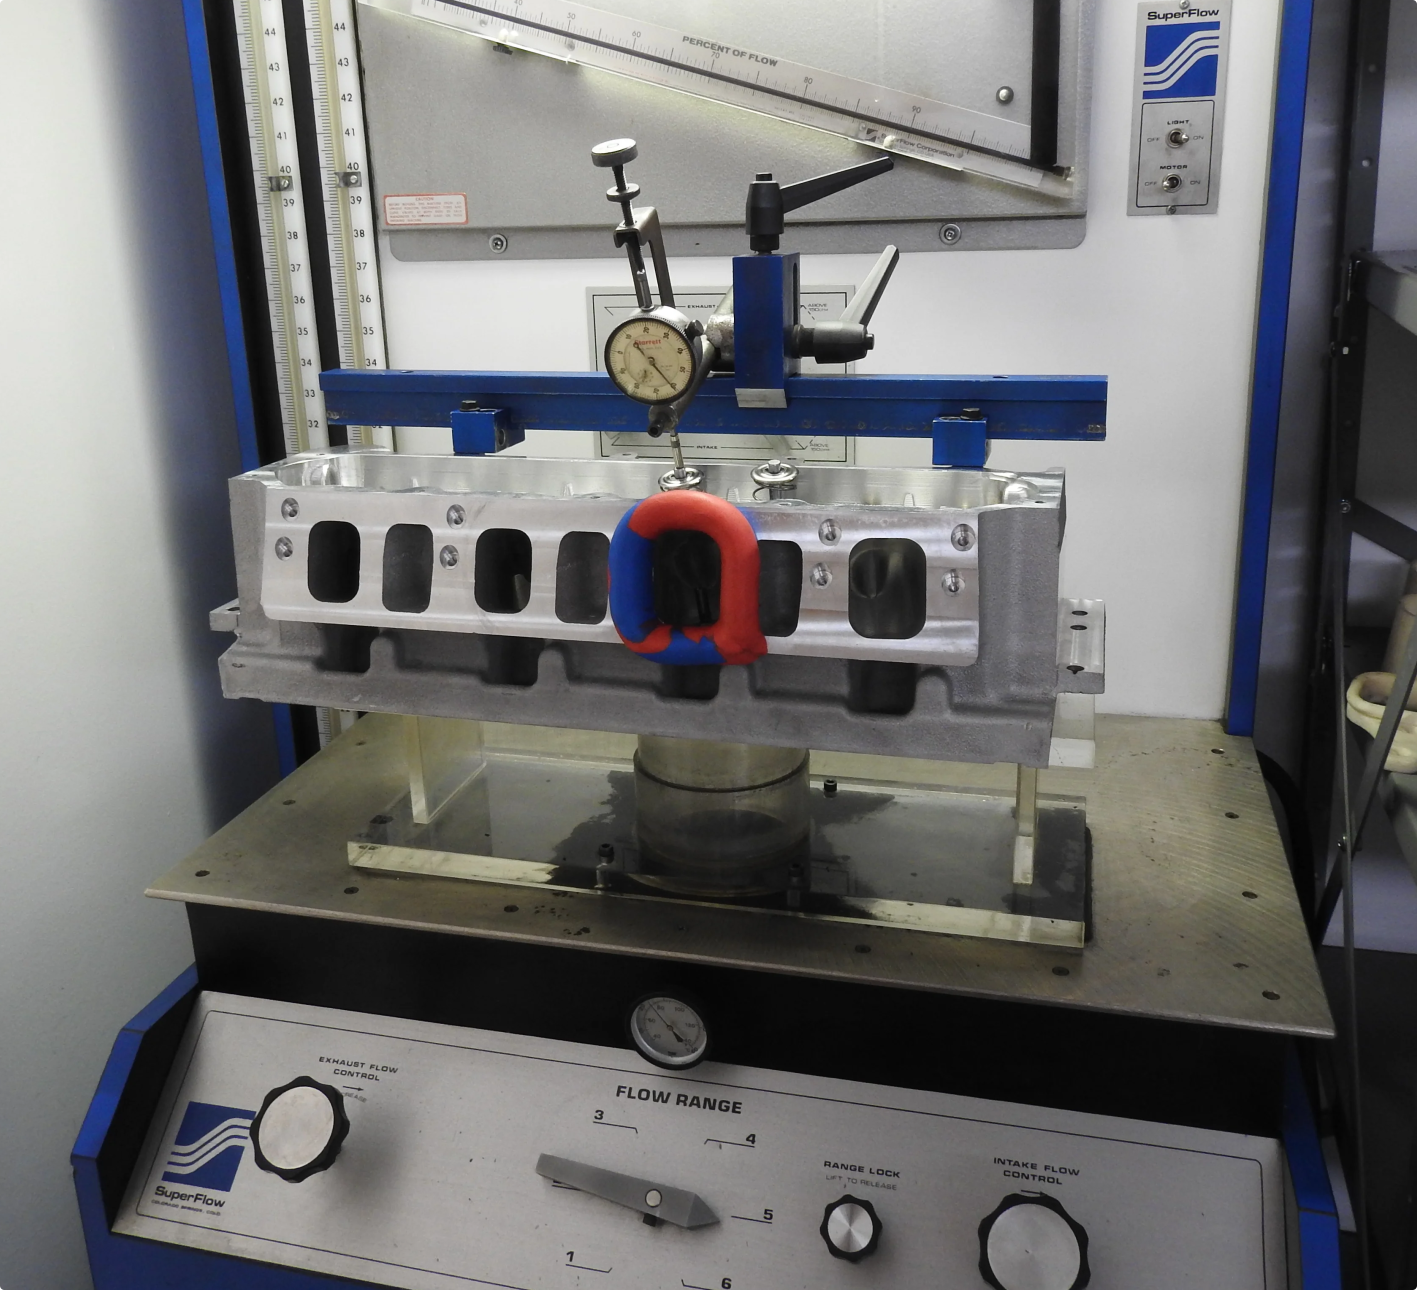
\includegraphics[width=0.5\textwidth]{./flujometrias/banco_flujometrias.png}
%
  \caption{Banco de flujometrías Super-Flow SF-750\protect\footnotemark}\label{fig:banco_flujometrias}
  %
\end{figure}

\footnotetext{\url{https://superflow.com/tech-corner/understanding-and-working-with-superflow-flowbenches/}}

Durante el ensayo se mide el caudal de aire atmosférico para diferentes grados
de apertura de la válvula y así se obtienen datos de (alzada, flujo) con los
cuales comparar entre diferentes geometrías de puertos de admisión o escape.
%
En la Figura~\ref{fig:flow-1} se muestra el resultado del ensayo de un
flujómetro en el que se compara la capacidad de flujo de dos tapas de cilindro
diferentes de un BMW S14
\footnote{\url{http://e30sport.net/tech_articles/engine-tech/flow-1/chart-1.htm}}.

\begin{figure}[h!]
  \centering
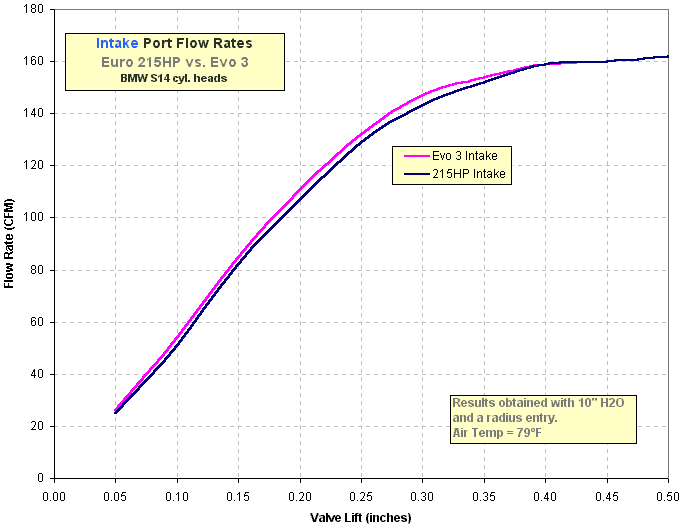
\includegraphics[width=0.8\textwidth]{./flujometrias/flow-1.png}
  \caption{Comparación entre flujometrías de dos tapas de cilindro de un BMW S14}\label{fig:flow-1}
\end{figure}

Otra forma de aproximar un coeficiente de descarga es por medio de flujometrías
computacionales.
%
El uso de CFD permite modelar el puerto en condiciones operativas, incluyendo
la interacción con elementos como por ejemplo el pistón, o en el caso del
MRCVC, estator y conjunto rotante.
%
Además, se pueden modelar las propiedades del fluido de trabajo para una
viscosidad, presión y temperatura representativas de las condiciones operativas
del motor que se está simulando.
%
En este trabajo se optó por esta metodología, es decir, a partir de las
flujometrías virtuales se obtuvo un valor de caudal másico el cual es utilizado
para calcular un coeficiente de descarga.

Conociendo el caudal másico $\dot{m}$, el valor de $C_{D}$  se calcula con las
ecuaciones de flujo compresible a través de una restricción, habiendo dos casos
distintivos: flujo bloqueado y no bloqueado.

Para el caso en que el flujo no esté bloqueado la ecuación de $\dot{m}$ es
la~(\ref{eq:m_no_bloqueado}) y en caso de que se cumpla la
desigualdad~(\ref{eq:cond_bloqueo}) el flujo está bloqueado y se utiliza la
ecuación~(\ref{eq:m_bloqueado}):
%

\begin{equation}\label{eq:m_no_bloqueado}
    \dot{m} = \frac{C_D A_R p_0}{\sqrt{R T_0}} {\left(\frac{p_T}{p_0} \right)}^{1/\gamma} {\left( \frac{2\gamma}{\gamma-1} \left[1- {(\frac{p_T}{p_0})}^{{(\gamma-1)}/\gamma} \right] \right)}^{1/2}
\end{equation}

\begin{equation}\label{eq:cond_bloqueo}
  \frac{p_T}{p_0} \le {[\frac{2}{\gamma+1}]}^{\gamma/(\gamma - 1)}
\end{equation}

\begin{equation}\label{eq:m_bloqueado}
  \dot{m}=  \frac {C_D A_R p_0} {{(R T_0)}^{1/2}} \gamma^{1/2} {\left( \frac{2}{\gamma+1} \right)}^{(\gamma+1)/(2(\gamma-1))}
\end{equation}

donde
\begin{itemize}
    \item $p_0$, es la presión de estancamiento antes de la restricción.
    \item $T_0$, es la temperatura de estancamiento antes de la restricción.
    \item $p_T$, es la presión estática justo después de la restricción.
    \item $A_R$, es el área de pasaje de flujo o de referencia.
    \item $\dot{m}$, es el caudal másico.
  \item $\gamma$, es el cociente de capacidades térmicas del gas.
\end{itemize}

\nomenclature[PO]{\(p_0\)}{Presión de estancamiento antes de la restricción}
\nomenclature[PO]{\(T_0\)}{Temperatura de estancamiento antes de la restricción}
\nomenclature[PO]{\(p_T\)}{Presión estática justo después de la restricción}
\nomenclature[G]{\(A_R\)}{Área de pasaje de flujo o de referencia}

El flujo está bloqueado si la velocidad en la garganta de la restricción
alcanza la velocidad sónica. 
%
Dada esta condición $\dot{m}$ alcanza un límite y reducir la presión aguas
abajo de la restricción no produce un aumento del caudal.
%
% La condición de flujo bloqueado se puede expresar en términos de la relación
% de presiones aguas arriba $p_{0}$ y aguas abajo de la restricción $p_{T}$.
%
Las presiones y temperaturas involucradas en el cálculo de $\dot{m}$ se pueden
medir u obtener de una simulación computacional del ciclo del motor.
%
\nomenclature[PO]{\(p,P\)}{Presión}

Un parámetro importante en las ecuaciones utilizadas para el cálculo del
coeficiente de descarga $C_{D}$ es el área de referencia $A_{R}$ que define el
área utilizada para calcular el caudal másico que circula por el puerto.
%
% En un motor con válvulas se suele tomar el área de cortina como el producto de
% la circunferencia de la válvula con la alzada, es decir:

La elección del área de referencia utilizada para el cálculo es arbitraria.
%
Sin embargo en un motor con válvulas se suele utilizar el área de cortina (ver
Figura~\ref{fig:area_cortina}) la cual es el producto del perímetro de la
cabeza y la alzada de válvula.

\begin{equation} \label{eq:area_cortina}
  A_R = A_C = \pi D_v l_v
\end{equation}

% \nomenclature[G]{\(A_R\)}{Área de pasaje de flujo o de referencia}
\nomenclature[G]{\(A_C\)}{Área de cortina}
\nomenclature[G]{\(D_v\)}{Diámetro de válvula}
\nomenclature[G]{\(l_v\)}{Alzada de válvula}

\begin{figure}[h!]
  \centering
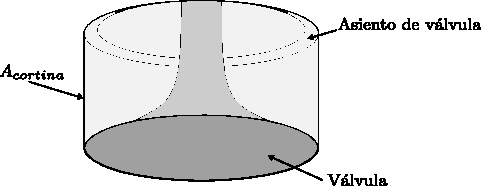
\includegraphics[width=0.5\textwidth]{valve_curtain.pdf}
  \caption{Área de cortina}\label{fig:area_cortina}
\end{figure}

Los valores de densidad, velocidad, presión y temperatura se obtienen de los
datos de salida de ICESym para un puerto, ángulo y velocidad dada.
%
Para la temperatura se utiliza la temperatura de la cámara, $T_0 = T_C$, la
presión antes y después del puerto se selecciona de acuerdo al sentido de
flujo.
%
En caso de ser hacia la cámara de combustión la presión en el puerto se utiliza
como valor a la entrada $P_0$ y la presión en la cámara es la aproximación a la presión en
la restricción $P_T$.
%
% TODO tengo que termiar de arreglar esta frase 15/11

Por otro lado, si el flujo ocurre en sentido contrario, desde la cámara hacia el
puerto, se utiliza la presión de cámara como valor de entrada $P_{0}$ y la
presión en el puerto es la presión en la restricción $P_{T}$.

El valor de $\gamma$ se obtiene de las propiedades de la mezcla con las rutinas
computacionales descritas en el apartado~\ref{subsec:prop_mezcla}.
%
\nomenclature[PO]{\(T\)}{Temperatura}
%
\nomenclature[SU]{\(0\)}{Valor inicial}
 \pagebreak

\chapter{HERRAMIENTAS COMPUTACIONALES}\label{capitulo:HERRAMIENTAS_COMPUTACIONALES}
\section{Internal Combustion Engine Simulator}
%
ICESym es un simulador de motores de combustión interna que  utiliza modelos 0D
para la cámara de combustión y 1D para el flujo a través del sistema de
intercambio de gases.
%
Esta combinación permite evaluar la \emph{performance} de un motor a un costo
computacional relativamente bajo; además la implementación de entrada y salida
de datos facilita utilizar el simulador como una \emph{caja negra}.
%
Esta característica permite incluir al simulador en un \emph{script} como una
función, a la cual se le otorga un conjunto de parámetros de entrada y devuelve
los resultados de la simulación en un formato que permite la lectura y
evaluación de los mismos.

ICESym contiene en su código las rutinas necesarias para simular el ciclo
operativo y la geometría del MRCVC.
%
Se realizaron modificaciones menores para facilitar la ejecución en conjunto con
el optimizador, algunas de estas modificaciones fueron:
%
\begin{enumerate}
    \item Modificar el formato de los archivos de salida, con el fin de reducir
el tamaño de los mismos, facilitar la lectura y el procesamiento de datos.
    \item Incluir una opción para elegir entre un modelo de $C_D$ de una o dos
variables.
    \item Modificar el área de referencia, ver Ecuación~\ref{eq:fv}.
    \item Agregar un esquema de interpolación bilineal que permita trabajar con
el modelo de $C_{D}$ de dos variables.
\end{enumerate}


\section{Modificaciones a ICESym}
%%%%%%%%%%%%%%%%%%%%%%%%%%%%%%%%%%%%%%%%%%%%%%%%%%%%%%%%%%%%%%%%%%%%%%%%%%%%%%%
\subsection{Flujo a Través de los Puertos}
%
Se introdujo una opción para poder ejecutar ICESym con un modelo del coeficiente
de descarga que dependa de dos variables: diferencia de presión y \emph{alzada}
o apertura del puerto, $C_D = f(lv; \Delta P)$.
%
Esto significó agregar un \emph{switch} en el código que permita seleccionar
entre un modelo de una o dos variables, con el agregado de las instrucciones de
lectura de datos y armado de un arreglo bidimensional que contiene los valores
del mapa de $C_{D}$ en un orden dado.
%
Con esto se construye un mapa del coeficiente de descarga de la forma $C_D =
f(lv, \Delta P)$, que se utiliza para calcular el área efectiva del puerto.

\nomenclature[F]{\(\Delta P\)}{Diferencia de presión a través de un puerto}

Independientemente de la cantidad de variables que formen parte del coeficiente
de descarga, a ICESym se introduce un vector para el caso 1D y una matriz para
el caso 2D.
%
El esquema de interpolación bilineal implementado requiere de una malla
rectangular.
%
Se reutilizó el código existente para el caso 1D, realizando una interpolación
lineal entre dos valores en planos con datos conocidos, como se ve en la
Figura~\ref{fig:interp_bilineal}.
%
Si bien hay otros métodos de interpolación para estimar el valor de $C_D$ a
partir de una nube de puntos, este método es sencillo y da resultados
satisfactorios.
%
En la Figura~\ref{fig:bilineal} se muestra a modo de ejemplo el error obtenido
con este método para interpolar una función de prueba
$f=\sin\left(\sqrt{x^2 + y^2}\right)$.

\begin{figure}
    \centering
    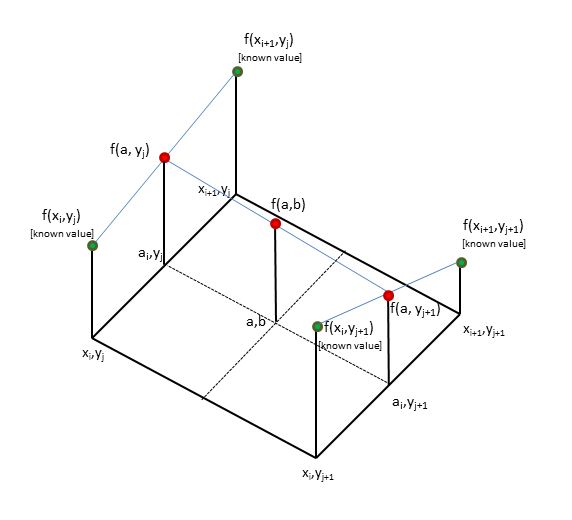
\includegraphics[width=0.7\textwidth]{interpolacion_bilineal.png}
    %
    \caption{Interpolación bilineal\protect\footnotemark}\label{fig:interp_bilineal}
    % \footnote{A}}
\end{figure}
\footnotetext{\url{https://stackoverflow.com/questions/8808996/bilinear-interpolation-to-enlarge-bitmap-images}}

\begin{figure}
    \centering
    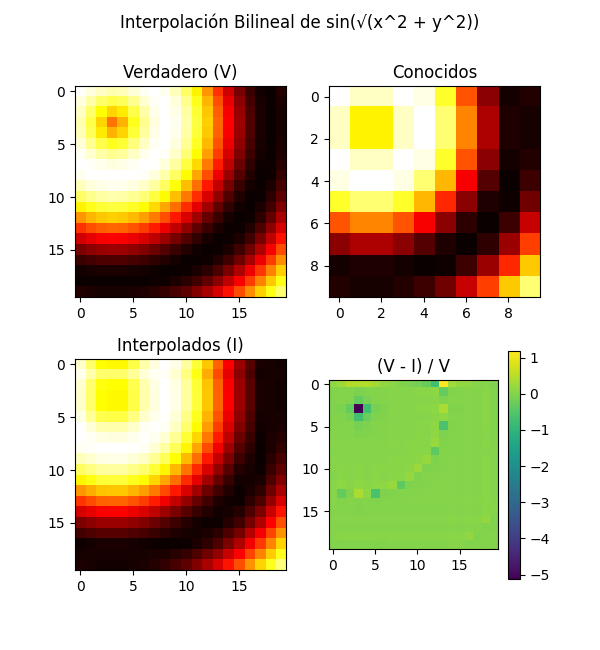
\includegraphics[width=0.6\textwidth]{bilineal.png}
    \caption{Interpolación bilineal de $\sin(\sqrt{x^2 + y^2})$}\label{fig:bilineal}
\end{figure}

La malla rectangular requerida para la interpolación bilineal del mapa de
$C_{D}$ se realizó a partir de los valores resultantes de las flujometrías con
\emph{OpenFOAM}~\parencite{openfoam}.
%
Debido al costo computacional que requieren las flujometrías, solo una cantidad
reducida de puntos se obtendrá con este método.
%
Se tiene como punto de partida una malla no rectangular, por lo que se utiliza
un método intermedio para obtener una matriz de puntos que pueda ser leída por
la interpolación bilineal.

Se probaron dos métodos para realizar esta interpolación, el método del punto más
cercano (MC) y la interpolación por la suma de la inversa de la distancia o IDW por
sus siglas en inglés (\emph{Inverse Distance Weighting}).
%
Estos se combinan con métodos de suavizado de promedio móvil con los $S$ valores
más cercanos.
%
Con este método cada valor original de la matriz se reemplaza por el promedio
aritmético de los valores a una distancia $S$ de cada celda evaluada.
%
En la Figura~\ref{fig:suavizado_promedio} se muestra este proceso para una
matriz de $5\times5$.

\begin{figure}[h!]
    \centering
    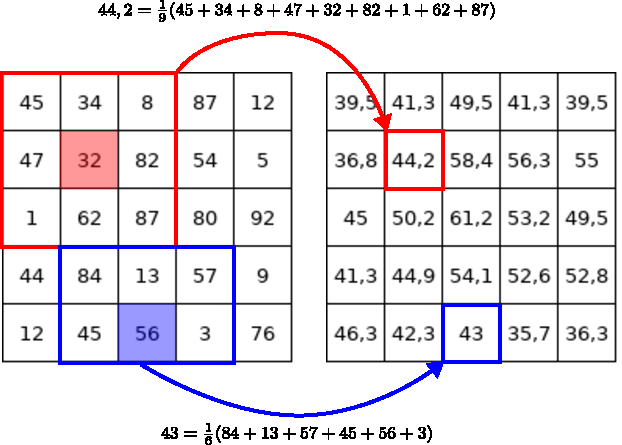
\includegraphics[]{/mapa_cd/suavizado.pdf}
    \caption{Suavizado por promedio con celdas vecinas, S=1}\label{fig:suavizado_promedio}
\end{figure}


El método del punto más cercano consiste en asignar para cada par $(x, y)$ el
valor conocido más cercano, ver Algoritmo~\ref{algo:mas_cercano}.

\begin{algorithm}
 \caption{Interpolación por punto más cercano}\label{algo:mas_cercano}
    \KwIn{\\
        $V_x, V_y$: valores de $x, y$ en los que se conoce el valor en $z$.\\
        $V_z$: valores conocidos de $z$.\\
        $I_x$: $n$ puntos de $x$ donde se quiere interpolar\\
        $I_y$: $m$ puntos de $y$ donde se quiere interpolar\\
        }

    \KwResult{Devuelve una matriz $I_{[n,m]}$ con los valores interpolados,
      donde a cada punto $I(x,y)$ se le asigna al valor de $v_z$ más cercano
      conocido. Da como resultado superficies escalonadas.}

    \BlankLine
     $I=zeros_{[n,m]}$\;
     \For{$i \gets 0$\KwTo$n$}{
        \For{$j \gets 0$\KwTo$m$}{
          $d = \sqrt{{(V_x - I_{xi})}^2 + {(V_y - I_{yj})}^2}$\;
            $I[i,j] = v_z[\min(d)]$\;
        }
     }
\end{algorithm}

La interpolación por IDW consiste en asignar a cada punto el resultado de un
promedio de los valores cercanos, ponderado por la distancia elevado a un
exponente arbitrario $p$.
%
Cuanto más grande el valor de $p$, más sensible es el método a los valores
cercanos.
%
La ecuación del promedio es la~(\ref{eq:idw}) y en el Algoritmo~\ref{algo:IDW}
se presenta el esquema utilizado.
%

\begin{equation} \label{eq:idw}
    f_p = \frac{\sum_{i=1}^{n} \frac{z_i}{d_i^p}} {\sum_{i=1}^{n}
    \frac{1}{d_i^p}}
\end{equation}

En la Figura~\ref{fig:mapas_interpolados} se muestra una comparación de ambos
métodos, para una malla de $C_{D}=f(\Delta P, l_{v})$ generada al azar.

\begin{algorithm}
    \caption{Interpolación IDW}\label{algo:IDW}
    \KwIn{\\
        $V_x, V_y$: valores de $x, y$ en los que se conoce el valor en $z$.\\
        $V_z$: valores conocidos de $z$.\\
        $I_x$: $n$ puntos de $x$ donde se quiere interpolar\\
        $I_y$: $m$ puntos de $y$ donde se quiere interpolar\\
        $p$: potencia a la que se eleva cada peso\\
        }

    \KwResult{Interpolación ponderada por inverso de la distancia. Dependiendo
      del valor de $p$, se obtienen valores más o menos suavizados.}

    \BlankLine
    $I=zeros_{[n,m]}$\;
    \For{$i \gets 0$\KwTo$n$}{
        \For{$j \gets 0$ \KwTo $m$}{
          $d = {\left[{(V_x - I_{xi})}^2 +{(V_y - I_{yj})}^2\right]}^{\frac{p}{2}}$\;
          \eIf{$\exists i : d[i] = 0$}{
            $I[i, j] = V_z[i]$\;
          }{
            $I[i,j] = \frac{\sum{V_{zi}/d_i}}{\sum \frac{1}{d}}$\;
          }
        }
     }
\end{algorithm}

% TODO:
% Modificar esto para mostrar la comparación entre métodos de interpolación con
% una función más convencional, como la que se ve en estas páginas:

% http://matlab.izmiran.ru/help/techdoc/math/poly_interp16.html
% https://medium.com/productive-data-science/how-to-interpolate-data-with-scipy-d314143285bc
% https://www.alglib.net/inverse-distance-weighting/
% https://www.mathworks.com/help/matlab/ref/peaks.html (peaks function)

\begin{figure}
    \centering
    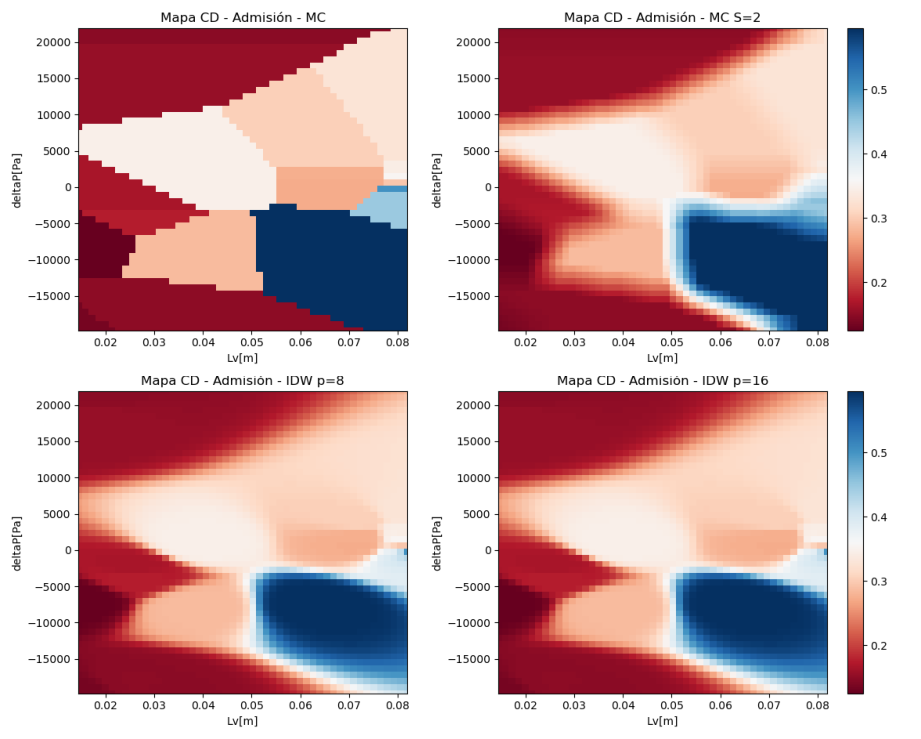
\includegraphics[width=.7\textwidth]{mapa_cd/mapa_cd.pdf}
    \caption{Comparación de métodos de interpolación}\label{fig:mapas_interpolados}
\end{figure}

%%%%%%%%%%%%%%%%%%%%%%%%%%%%%%%%%%%%%%%%%%%%%%%%%%%%%%%%%%%%%%%%%%%%%%%%%%%%%%%

\subsection{Área de Referencia}
%
El área de referencia utilizada por ICESym es el área de la cortina~(ver
Ec.~\ref{eq:area_cortina}) y se emplea en el código del programa para calcular
el área efectiva $F_{V}=A_{R}\cdot C_{D}$.
%
Como se indicó en el apartado~\ref{sec:cap2_cd}, para el  MRCVC el área de
referencia es el área frontal del puerto expuesta a la cámara, calculada como la
altura de la ranura $h_{p}$ multiplicada por la distancia entre el borde del
puerto y la paleta que delimita la cámara, denominada como $l_{v}$.

Este valor se afecta por el coeficiente de descarga intermedio $C_{D,int}$, que
puede ser un valor fijo o el resultado de interpolar de un mapa de $C_D$ para un
valor de cuerda y $\Delta P$ dado, como se indica en la ecuación~(\ref{eq:fv}).

\begin{equation}\label{eq:fv}
    F_{V} = C_{D,int}\cdot h_{p}\cdot l_{v}
\end{equation}

Tanto al inicio como al cierre del puerto ocurre solape de cámaras, por lo que
en estos intervalos angulares hay un valor de $C_D$ para cada cámara.
%
Cada valor se calcula con el flujo másico que atraviesa las secciones de entrada
correspondientes y el área de puerto expuesta por cada cámara.

\subsection{Interfaz con el Optimizador}
%
Para lograr ejecutar el simulador automáticamente, se creó una librería de
funciones capaz de tomar como dato de entrada un archivo de configuración que
incluye geometría, velocidades a ejecutar y cantidad de ciclos de simulación,
entre otros.

Para ejecutar una instancia de ICESym se puede utilizar la interfaz gráfica de
usuario (GUI) ó ejecutarlo por línea de comando desde una consola.
%
El simulador de motores se ejecuta como un archivo de Python {\tt>{}> python main.py}, el cual contiene las instrucciones que lanzan la simulación del
motor con la configuración requerida.
%

ICESym requiere de un archivo de configuración con los datos de la simulación a
realizar, este archivo se organiza como sigue:
\newline

\begin{forest}
  [config.py
    [Atmospheres]
    [Junctions]
    [Simulator]
    [Cylinders
      [Combustion]
      [Fuel]
      [Inyection]
      [Valves]]
    [Tanks]
    [Tubes]
  ]
\end{forest}

\begin{itemize}
  \item {\tt Atmospheres}: contiene el estado de la atmósfera, que es condición de
contorno de la simulación: presión, densidad y velocidad inicial.
  \item {\tt Cylinders}: geometría y condiciones de contorno, estado inicial,
tipo de motor, como así también de las válvulas.
  \item {\tt Valves}: geometría, tipo de válvula, modelo de $C_{D}$, perfil de alzada y
datos de $C_{D}$ y tubo conexionado.
  \item {\tt Junctions}: contiene información de las uniones entre tubos.
  \item {\tt Simulator}: configuración de la simulación, velocidades a simular,
propiedades de gas, tipo de motor, directorios, entre otros.
  \item {\tt Tanks}: volumen, masa y temperatura de pared de tanques.
  \item {\tt Tubes}: geometría, cantidad de nodos y conexiones de los tubos.
\end{itemize}

Los elementos de configuración intervenidos por el optimizador son {\tt
Cylinders}, {\tt Valves}, {\tt Simulator} y {\tt Tubes}; donde se  modifican los
siguientes valores:

\begin{itemize}
  \item {\tt Simulator}:
        \begin{itemize}
          \item {\tt RPMS}: Velocidades a simular (por ejemplo una lista de [1000,
2000, \ldots, 9000].
          \item {\tt NCYCLES}: cantidad de ciclos por velocidad (un entero mayor o igual a 1).
          \item {\tt FOLDER NAME}: nombre de la carpeta donde se guardan los
resultados de la simulación.
          \item {\tt SHOW INFO}: selector para mostrar o no información de la simulación.
          \item {\tt CONFIG DATA}: archivo donde se guarda la configuración utilizada.
        \end{itemize}
  \item {\tt Cylinders} $\longrightarrow$ Valves
        \begin{itemize}
          \item {\tt LvI}: perfil de alzada del puerto de admisión.
          \item {\tt LvE}: perfil de alzada del puerto de escape.
          \item {\tt IPO}: ángulo de apertura del puerto de admisión.
          \item {\tt IPC}: ángulo de cierre del puerto de admisión.
          \item {\tt EPO}: ángulo de apertura del puerto de escape.
          \item {\tt EPC}: ángulo de cierre del puerto de escape.
          \item {\tt cd\_model}: selector de modelo de $C_{D}$.
                \begin{itemize}
                  \item $C_{D}l_{v}$ valores de alzada para el mapa de $C_{D}$(
para modelo de 2 variables).
                  \item $C_{D}d_{p}$ valores de $\Delta P$ para el mapa de
$C_{D}$ (para modelo de 2 variables).
                  \item $C_{D}$ valores de $C_{D}$ relacionados con alzada (para modelo de 1 variable).
                \end{itemize}
          \item $D_{v}$: diámetro de la cabeza de la válvula.
        \end{itemize}
  \item Tubes
        \begin{itemize}
          \item longitud: longitud total del tubo de admisión o escape.
        \end{itemize}
\end{itemize}

Los valores de alzada y diámetro de válvula son valores utilizados en la
configuración anterior no se corresponden con magnitudes geométricas en el
MRCVC.
%
Estos valores se introducen como datos con el requisito de que el área de
cortina ($A_{C}$) coincida con el área de referencia ($A_{R}$).

%%%%%%%%%%%%%%%%%%%%%%%%%%%%%%%%%%%%%%%%%%%%%%%%%%%%%%%%%%%%%%%%%%%%%%%%%%%%%%%%
%%%%%%%%%%%%%%%%%%%%%%%%%%%%%%%%%%%%%%%%%%%%%%%%%%%%%%%%%%%%%%%%%%%%%%%%%%%%%%%%
%%%%%%%%%%%%%%%%%%%%%%%%%%%%%%%%%%%%%%%%%%%%%%%%%%%%%%%%%%%%%%%%%%%%%%%%%%%%%%%%


\section{Optimizador y Algoritmo Genético}
%
% Se seleccionó un algoritmo genético (AG) como método de optimización por ser un
% método sencillo de programar además, este tipo de algorimto es de utilidad
% cuando se tiene una solución con uno o más máximos óptimos locales ó cuando no
% se tiene certeza sobra la suavidad de la función a evaluar.
%

Se seleccionó un algoritmo genético (AG) para realizar la optimización de la
geometría del MRCVC por la simplicidad y facilidad de implementación del mismo.
%
Si bien este tipo de métodos no garantiza que se alcance un resultado óptimo,
en la práctica se ha observado que alcanzan soluciones muy cercanas a las
óptimas tras pocas iteraciones del método~\parencite{goldberg};\parencite{shi}.

Una de las ventajas de este método es que no requiere información del gradiente
de la función que se está evaluando, lo cual es útil cuando no se puede asegurar
la existencia de la derivada de la función en todo el dominio ó cuando se tiene
una función con más de un máximo o mínimo local.
%
Además, como el punto de partida de la optimización es una población generada al
azar, se tiene un muestreo aleatorio del dominio que se está evaluando.
%
Esto hace que el método sea poco susceptible a dar como resultado óptimos
locales.

Se puede decir que un algoritmo genético es un método de búsqueda aleatoria
guiada.
%
¿Cómo difieren los AG de los métodos tradicionales de búsqueda?
%
\begin{enumerate}
  \item Los AG pueden operar sobre una representación de las variables estudiadas y
no necesariamente sobre las variables de estudio.
  \item Cada iteración utiliza un conjunto de datos con cierto grado de
aleatoriedad.
  \item Utilizan una función objetivo para evaluar cada punto sin necesidad de
conocer la derivada de la función que se está evaluando.
  \item Los AG usan reglas probabilísticas de decisión.
\end{enumerate}


% \subsection{Componentes básicos de un AG}
%
Los mecanismos básicos que hacen a un algoritmo genético son: 1) \emph{selección}, 2)
\emph{cruza} y 3) \emph{mutación}.
%
El funcionamiento básico se sintetiza en el Algoritmo~\ref{algo:genetico}.

La \emph{selección} consiste en crear individuos a partir del puntaje que devuelve
una función objetivo, la cual es la encargada de guiar el proceso de
optimización dando mayor o menor puntaje a un candidato según el resultado que
se quiere obtener.
%
Este paso significa que, aquellos individuos a los cuales se les asignó un
puntaje más elevado tienen más probabilidades de ser copiados o de
``transmitir'' sus parámetros a la iteración siguiente.
%
Este proceso imita en cierta forma la selección natural o evolución Darwiniana y
de aquí viene el nombre de algoritmo genético o evolutivo.

El segundo operador es la \emph{cruza}, que consiste en combinar los parámetros
de dos individuos para obtener uno nuevo, esto se asemeja a la reproducción.

Finalmente la \emph{mutación} es la encargada de modificar aleatoriamente uno o más
parámetros de cada nuevo individuo.
%
Este operador juega un rol secundario pero muy importante en la simulación.
%
Es secundario porque se pueden alcanzar soluciones satisfactorias sin que se
aplique este operador en la población.
%
Es importante porque utilizando probabilidades pequeñas de ocurrencia (de la
mutación), permite evitar la pérdida temprana de información relevante por
convergencia temprana de la simulación.
%
Por otro lado, en caso de que la probabilidad de mutación sea muy alta, el AG se
convierte en un método de búsqueda aleatoria.

\begin{algorithm} \caption{Algoritmo de optimización}\label{algo:genetico}
  Inicializar población, al azar o a partir de una población ``semilla''\;
  %
  \While{no se cumpla condición de parada}{
    %
    \emph{Seleccionar} a los individuos más aptos, evaluándolos según la función objetivo\;
    %
    \emph{Cruzar} los candidatos seleccionados para crear la nueva población (la
próxima iteración del método)\;
    %
    \emph{Mutar} algunos individuos de la nueva población\;
    %
    \If{se cumple la condición de parada}{
      Parar\;
    }
  }
  {Guardar resultados\;}
\end{algorithm}

Gran parte de este trabajo consistió en adaptar el uso de ICESym y emplearlo
como base para generar una función objetivo, aprovechando la cualidad de ``caja
negra'' con la que se puede implementar el simulador.
%
Para lograr esto se modificó parte del código de ICESym con el objetivo de
facilitar la configuración, ejecución y lectura de los resultados que arroja el
simulador y así poder ejecutar de manera automática una simulación con una
configuración particular del motor.
%
Otro aspecto del optimizador que se desarrolló, es el de poder ejecutar
múltiples instancias de ICESym en paralelo con el fin de reducir el tiempo de
ejecución de cada generación, pudiendo evaluar varios motores (o individuos) al
mismo tiempo.

Para la primera iteración se programaron desde cero los algoritmos y funciones
necesarias para llevar a cabo la optimización con el AG.
%
Posteriormente se tomó la librería DEAP~\parencite{DEAP_JMLR2012} y se
modificaron los operadores a medida, para poder utilizarlos con ICESym.

En los apartados siguientes se describe la implementación de cada uno de los
operadores en el optimizador.

\subsection{Población}
%
Se decidió representar cada motor como un vector con las dimensiones y reglaje
que definen la geometría del sistema de intercambio de gases, los cuales se
listan en la Tabla~\ref{tab:param_motor}.
%
Se limitaron los valores que puede tomar cada parámetro para que la geometría
resultante se asemeje a la geometría del motor utilizado en trabajos anteriores,
aprovechando así los resultados obtenidos en el primer barrido paramétrico.

\begin{table}[h!]
  \centering
  \begin{tabular}{rllll} \toprule
    Nº & Parámetro & Descripción & Sistema & Límites \\ \midrule
    1 & DTA & Diámetro de tubo & Admisión & [60, 100] mm \\
    2 & DTE & Diámetro de tubo & Escape & [60, 100] mm\\
    3 & LIT & Largo de tubo & Admisión & [300, 2000] mm\\
    4 & LET & Largo de tubo & Escape & [300, 2000] mm\\
    5 & IIA & Ángulo geométrico de apertura & Admisión & [0,90]º \\
    6 & IFA & Ángulo geométrico de cierre & Admisión & [IIA, 90]º \\
    7 & IIE & Ángulo geométrico de apertura & Escape & [0, 90]º \\
    8 & IFE & Ángulo geométrico de cierre & Escape & [IIE, 90]º \\ \bottomrule
  \end{tabular}
  \caption{Parámetros que representan al motor}\label{tab:param_motor}
\end{table}

Los vectores que hacen a cada motor se representan como un número binario de 40
dígitos, ocupando 5 dígitos para representar cada uno de los 8 parámetros que
hacen a cada motor.
%
Esto facilita la implementación de los operadores de selección, cruza y
mutación, pudiendo aprovechar implementaciones de operadores existentes en
librerías como DEAP.
%
Estos 8 números binarios luego se convierten en una lista de enteros mediante
una transformación lineal $f(x)=a\cdot x+b$, en la que se ingresa con un entero
entre 0 y $2^{n}-1$ para ir del número binario a un decimal, siendo $n$ la
cantidad de dígitos del número binario (en este caso 5).
%
Los coeficientes $a$ y $b$ son tales que $f(0)=x_{0}$ y $f(2^{n}-1) = x_{1}$,
donde $x_{0}$ y $x_{1}$ son los extremos del rango para el que se quiere aplicar
la transformación.
%
Estos coeficientes ($a$ y $b$) son particulares a cada parámetro, porque se
determinan de acuerdo a los valores que puede tomar cada uno.

De este modo se obtiene el valor de cada uno de los parámetros que hacen a la
configuración particular de cada motor en ICESym.
%
El orden de los mismos se mantiene constante, por lo que cada sección del número
representa una característica en particular del motor.

A modo de ejemplo, en la Figura~\ref{fig:pop_bit} se muestra un número generado
aleatoriamente, la transformada para los primeros 5 dígitos que corresponden al
diámetro del tubo de admisión, 00111.
%
Si se desea que el diámetro del tubo de admisión varíe entre 60 y 100 mm, se
deben obtener los coeficientes $a$ y $b$ para la transformación lineal  a partir
del largo del número binario que se va a utilizar, {\tt{binLen}}, y los valores
mínimos y máximos del rango sobre el que se quiere transformar el valor de
entrada: $vMin=60$ y $vMax=100$.

Los coeficientes $a$ y $b$ se obtienen a partir de:
\begin{align*}
  a &= \frac{vMax-vMin}{2^{binLen} - 1} =\frac{100-60}{2^{5}-1} = 1,2903\\
  b &= vMin=60
\end{align*}

Luego, el número binario transformado a entero vale:
\begin{equation*}
  00111 \longrightarrow 0\cdot 2^{4} + 0\cdot 2^{3} + 1\cdot 2^{2} + 1\cdot 2^{1} + 1\cdot 2^{0} = 7
\end{equation*}

Finalmente, con los coeficientes ($a$, $b$) y el binario transformado en entero,
se tiene que DTA vale

\begin{equation*}
  DTA = a\cdot x + b = (1,2903\cdot 7 + 60) = 69 mm = 0,069 m
\end{equation*}


\begin{figure}[h!]
  \centering
  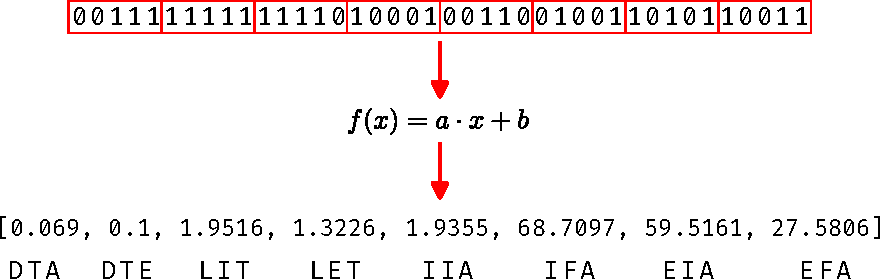
\includegraphics[]{genetico/map_to_engine.pdf}
  \caption{Representación del individuo}\label{fig:pop_bit}
\end{figure}


\subsection{Selección}

Para crear la nueva población se debe elegir a los nuevos candidatos basándose
en los puntajes de la población actual.
%
Hay varios métodos diferentes de selección, como lo son de ruleta, aleatoria,
por puntaje y de tipo torneo.
%
Para este trabajo se seleccionó el método de torneo, el cual es uno de los
métodos más populares para los procesos de selección de AG.

El método consiste en seleccionar $k$ individuos de la población al azar, se
comparan los puntajes de estos individuos y resulta ``ganador'' aquel que tenga
más puntaje.
%
El proceso se repite $N$ veces hasta generar la nueva población.

El parámetro $k$ es el tamaño de torneo y comúnmente se utiliza
2~\parencite{oladele}.
%
A mayores valores para $k$ se tiene una mayor pérdida de diversidad en los
resultados~\parencite{blickle} porque reduce la posibilidad de que candidatos con
menor puntaje sean seleccionados para la nueva generación (convergencia
temprana).

Para este torneo se utilizó además un \emph{salón de la
  fama}~\parencite{wirsansky} de 1 individuo.
%
Esto significa que el mejor individuo de la población actual es automáticamente
seleccionado para la iteración siguiente y la selección por torneo se realiza
$N-1$ veces.

\subsection{Cruza}
%
El operador de cruza se encarga de combinar los genes  de dos individuos para
producir uno nuevo.
%
Se encarga de combinar/intercambiar los parámetros de los individuos
``cruzados'' para generar uno nuevo.
%
Para individuos representados por un vector se suelen usar operadores de tipo
cruza de uno o múltiples puntos, también se utilizan mecanismos de cruza
uniforme.
%
El método seleccionado es \emph{cruza de dos puntos}.
%
En este método se corta el vector que forma al individuo en dos puntos, la
posición de estos puntos se selecciona al azar, manteniendo el largo original de
los vectores.
%
Los individuos ``cruzados'' se combinan de forma complementaria como se indica
en la Figura~\ref{fig:cr2puntos}, el algoritmo~\ref{algo:cr2puntos} esquematiza
el proceso.

\begin{figure}[h!]
  \centering
  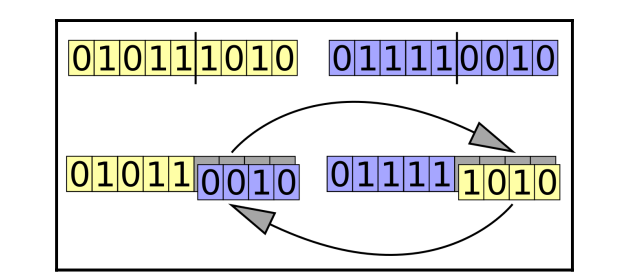
\includegraphics[width=0.5\textwidth]{cruza2puntos.png}
  \caption{Cruza de dos puntos~\parencite{wirsansky}}\label{fig:cr2puntos}
\end{figure}


\begin{algorithm}[h!]
  \KwIn{\\
    $ind_{1}, ind_{2}$: dos individuos de entrada, por ej. [101\ldots011], [110\ldots100].\\
    EA(a, b): devuelve un entero al azar entre los enteros a y b.\\
    L(a): devuelve la cantidad de elementos en a.}
  \KwOut{\\
    $ind_{1}, ind_{2}$: individuos de entrada modificados}
  \SetKwFunction{EA}{EA}
  \SetKwFunction{L}{L}
  % \SetKwFunction{min}{min}
  \BlankLine
  s = min(\L{$ind_{1}$}, \L {$ind_{2}$})\;
  $CX_{1} = \EA{1, s}$\;
  $CX_{2} = \EA{1, s-1}$\;
  \eIf{$CX_{1} \geq CX_{2}$}{
    $CX_{2} = CX_{2}+1$\;
  }{
    $aux=CX_{1}$\;
    $CX_{1}=CX_{2}$\;
    $CX_{2}=aux$\;
  }
  $aux = ind_{1}$\;
  $ind_{1}[CX_{1}:CX_{2}] = ind_{2}[CX_{1}:CX_{2}]$\;
  $ind_{2}[CX_{1}:CX_{2}] = aux[CX_{1}:CX_{2}]$\;
  \Return{$ind_{1}, ind_{2}$}\;
  \caption{Cruza de dos puntos}\label{algo:cr2puntos}
\end{algorithm}

\subsection{Mutación}
%
La mutación juega un rol secundario pero importante en los AG, consiste en
modificar aleatoriamente alguno de los parámetros que definen a un individuo.
%
Este mecanismo contribuye a la diversidad de soluciones y por ende reduce la posibilidad de
convergencia temprana.
%
Se utilizan probabilidades bajas de mutación, en el caso extremo si la
probabilidad de mutación es del $100\%$ el AG se convierte en un método de
búsqueda aleatoria.
%
Algunos de los métodos de mutación utilizados son:

\begin{description}
  \item [Flip Bit] es uno de los métodos más simples y comunes. En la
representación binaria de un cromosoma, se selecciona uno o más bits al azar y
se invierten. Es decir, si el bit es 1, se cambia a 0 y viceversa.
        %
  \item [Intercambio] en este método se seleccionan dos posiciones en el
cromosoma de manera aleatoria y se intercambian los valores de estas posiciones.
        %
  \item [Inversión] se elige un segmento dentro del cromosoma y se invierten los
elementos de ese segmento. Por ejemplo, en la secuencia [A, B, C, D, E],
se invierten los elementos B y D, obteniendo [A, D, C, B, E].
        %
  \item [Reordenado Aleatorio] se selecciona un subconjunto de genes en el
cromosoma y se reordenan aleatoriamente. A diferencia del método de inversión,
los genes no se voltean simplemente de posición, sino que además pueden terminar
en cualquier orden.
\end{description}

En este trabajo se utiliza el método de reordenado aleatorio en el cual se
modifica al azar el orden de los números que hacen al individuo, modificando los
índices de la lista que define el arreglo, por ejemplo: $11100 \rightarrow 10011$.
%
El pseudocódigo de este proceso se presenta en el algoritmo~\ref{algo:flipbit}.

\begin{algorithm}
  \caption{Flip Bit}\label{algo:flipbit}
  \DontPrintSemicolon
  \KwIn{
    $A = (a_{1}, a_{2}, \ldots, a_{n})$ es un vector compuesto de unos y ceros.\\
    $R$, es una función aleatoria que devuelve un número real entre 0 y 1.\\
    $p$, es un número real entre 0 y 1 que representa la probabilidad de mutación.
  }

  \For{i=1 \KwTo n}{
    \If{$R < p$}{
      \lIf{$A_{i}=1$}{$A_{i}=0$}
      \lElse{$A_{i}=1$}
      }
  }
    \Return A\;
\end{algorithm}

\subsection{Función Objetivo}\label{sec:funcion_objetivo}
%
La función objetivo es la encargada de dar puntaje a los individuos, en la
analogía con la selección natural esta función es el ambiente.
%
Determina la aptitud de un motor con respecto a otro en lo que respecta a
\emph{performance} del sistema de intercambio de gases.
%
Inicialmente se propuso que la función objetivo sea la suma de los rendimientos
volumétricos a todas las velocidades simuladas $s=\sum \eta_{v}$.
%
Este tipo de funciones dió como resultado una curva de $\eta_{v}$ aserrada como
se muestra en la Figura~\ref{fig:curva_aserrada}.

\begin{figure}[h!]
  \centering
  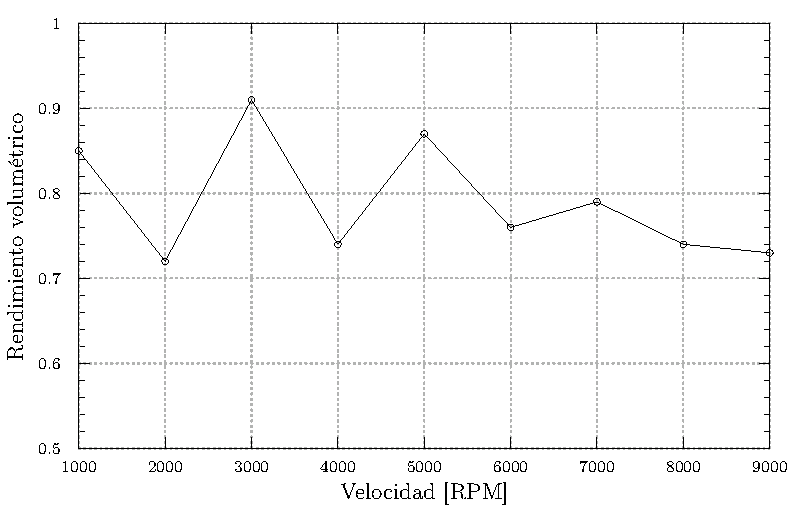
\includegraphics[width=0.7\textwidth]{gnuplot/rendimiento_aserrado.pdf}
  \caption{Curvas de rendimiento volumétrico aserradas}\label{fig:curva_aserrada}
\end{figure}

Esta curva aserrada es poco deseable porque significa una entrega de torque y
potencia dispar, por este motivo se modificó la función objetivo para favorecer
curvas suaves y preferentemente con un solo punto de inflexión.
%
Se implementó una suma ponderada para obtener un rendimiento volumétrico máximo
en un valor cercano a 6000 RPM de modo de aprovechar las características de
balanceo de fuerzas y mayores velocidades de giro de los motores rotativos.
%
La aptitud resulta de la suma del rendimiento volumétrico y el inverso de la
fracción de gases residuales, lo cual probó ser la función objetivo que mejores
resultados dió.
%p
La metodología utilizada se resume a continuación.

\begin{enumerate}
        \item Se evalúa cada motor, calculando el rendimiento volumétrico
$\eta_{v}$ y la fracción de gases residuales $x_{r}$ para cada velocidad de giro
simulada.
        \item Con $\eta_{v} = (\eta_{v,1}, \ldots ,\eta_{v,n})$ y
$x_{r}=(x_{r,1},\ldots,x_{r,n})$ se realiza la siguiente suma para cada velocidad
$S_{i}=\eta_{v,i} + x_{r,i}^{-1}$.
        \item Cada motor tiene un vector o lista de valores
$S = (S_{1},\ldots,S_{n})$ para cada velocidad evaluada, con la cual se calcula
el puntaje del motor como:
        \begin{equation}
        f = \sum_{i=1}^{n}{S_{i}} + S_{k}^{2}
      \end{equation}

El valor $S_{k}$ es el puntaje para la $k$-\textit{ésima} velocidad de giro (6000 RPM en
este caso) y se eleva al cuadrado para favorecer altos rendimientos en esta
velocidad.
\end{enumerate}


Durante las primeras iteraciones del método hay una gran cantidad de geometrías
inválidas que devuelven puntaje muy bajo o nulo.
%
En caso de que alguna de las soluciones tenga un puntaje relativamente alto,
existe la posibilidad de una dominancia temprana de la población, provocando
una convergencia temprana de la optimización.
%
Estos candidatos tienen una mayor probabilidad de ``pasar'' sus características
geométricas a las iteraciones siguientes y es algo especialmente problemático en
optimizaciones con poblaciones de alrededor de 100 individuos.

Para reducir la posibilidad de una convergencia temprana se utiliza un método de
escalado de puntajes, que consiste en una transformación lineal en la que se
define el puntaje bruto de un individuo como $f$ y el puntaje escalado como
$f'$, la relación entre ambos es $f' = a\cdot f + b$.
%
Los coeficientes $a$ y $b$ se determinan de modo que $f'_{media}=f_{media}$, de
este modo un motor con puntaje promedio tiene la misma influencia sobre la
población ya sea con la aptitud original o escalada.
%
Para controlar la influencia del mejor individuo de una generación sobre la
próxima, los puntajes se transforman de tal modo que
$f'_{max}=C_{mult}f_{media}$.
%
El valor de $C_{mult}$ es la cantidad de copias que se espera obtener del mejor
de los candidatos en la generación siguiente y se usa en $1,2$ a $2$ para
poblaciones de entre 50 y 100 individuos~\parencite{goldberg}.

Hacia el final donde la diferencia entre puntajes de los individuos de la
población tiende a achicarse, el parámetro $C_{mult}$ cumple la función de
acrecentar las diferencias entre individuos.

En caso de existir individuos con puntaje muy bajo o nulo se hace un
pre-escalado del puntaje que fija el mínimo en $f'_{min}=0$.
%
El procedimiento se lista en los algoritmos \ref{algo:pre-escala} y
\ref{algo:pop_scale}.


\begin{algorithm} \caption{Algoritmo de pre-escalado}\label{algo:pre-escala}
  \KwIn{\\
    $F$, es un vector que contiene los puntajes de todos los individuos\;\\
    $C_{mult}$, es un multiplicador para el escalado, se suele usar
$C_{mult}\in[1.2, 2]$\;\\ }
  \KwOut{\\
    $a, b$, son los coeficientes para la transformación lineal $f(x)=a\cdot x + b$\;
  }
  \SetKwFunction{max}{max}
  \SetKwFunction{min}{min}
  \SetKwFunction{media}{media}
  \BlankLine

  $u_{max} = \max{F}$\;
  $u_{min} = \min{F}$\;
  $u_{medio} = \media{F}$\;
  \eIf{$u_{min}> aux = (C_{mult}\cdot u_{medio} - u_{max}) \mathbin{/} (C_{mult}-1)$
    }{
    $\Delta_{u} = u_{max}-u_{avg}$\;
    $a = (C_{mult} - 1) \cdot u_{avg} / \Delta u$\;
    $b = u_{avg} \cdot (u_{max} - C_{mult} \cdot u_{avg}) \Delta_{u} $\;
  }{
    \eIf{$\Delta \neq 0$}{
      $a = u_{avg} \mathbin{/} \Delta_{u}$\;
      $b = -u_{min} \cdot u_{avg} \mathbin{/} \Delta_{u}$ \;
    }{
      $a=1$\;
      $b=0$\;
    }
  }
  \Return{$a, b$}
\end{algorithm}


\begin{algorithm}\caption{Escalado de población}\label{algo:pop_scale}
  \KwIn{\\
    $f$, es la aptitud.\\
    $a, b$, son los parámetros de la función de pre-escalado. \\
  }
  \KwOut{\\
  $f^{*}$, los puntajes escalados.}
  \SetKwFunction{ps}{PreEscalado}
  \SetKwFunction{ll}{Largo}
  \SetKwFunction{esc}{Escala}
  \BlankLine

  $a, b = \ps{f, 2}$\;
  $f^{*} = ()$ \;
  $n = \ll{f}$\;
  \For{$i=1$ \KwTo $n$}{
    $f^{*}_{i} = a\cdot f_{i} + b$\;
  }
  \Return{$f^{*}$}\;
\end{algorithm}

% Con la población definida se procede a los evaluar cada motor con la función
% objetivo, la cual se definió de manera tal de favorecer curvas de rendimiento
% volumétrico suaves y valores altos a mayores RPM.\@

% La suavidad de la curva de rendimiento volumétrico se calcula midiendo los
% cambios de pendiente de la derivada la cual se aproxima con la fórmula de
% diferencia progresiva~\ref{eq:derivada}.
% %
% Solamente interesa el signo, por lo que el valor de $h$ en el denominador no
% interesa y se hace 1, con esto la función objetivo queda como el
% algoritmo~\ref{alg:funcObj}.

% \begin{equation}\label{eq:derivada}
%   f' = \frac{f(i+1) - u(i)}{h}
% \end{equation}

% Una vez evaluados todos los motores de la población, se debe seleccionar los
% individuos que formarán la siguiente iteración del algoritmo.
% %
% El método de selección es de tipo TORNEO, en el cual se seleccionan los mejores
% $k$ individuos de un grupo al azar de $N$ candidatos.
% %

% Con los nuevos candidatos seleccionados, se procede a variar la población,
% realizando la cruza y mutación.

% Luego se toman pares de individuos y de acuerdo a la probabilidad de cruza, se
% combinan con el método seleccionado.

% Finalmente se realiza una segunda iteración sobre la nueva población, aplicando
% el método de mutación a cada individuo, de acuerdo a la probabilidad de
% mutación indicada.
%

%%%%%%%%%%%%%%%%%%%%%%%%%%%%%%%%%%%%%%%%%%%%%%%%%%%%%%%%%%%%%%%%%%%%%%%%%%%%%%%%
%%%%%%%%%%%%%%%%%%%%%%%%%%%%%%%%%%%%%%%%%%%%%%%%%%%%%%%%%%%%%%%%%%%%%%%%%%%%%%%%
%%%%%%%%%%%%%%%%%%%%%%%%%%%%%%%%%%%%%%%%%%%%%%%%%%%%%%%%%%%%%%%%%%%%%%%%%%%%%%%%

\section{OpenFOAM}\label{sec:3_openfoam}
%
Las flujometrías se realizaron con \emph{OpenFOAM}, un software de
Fluidodinámica Computacional, o CFD por sus siglas en inglés, de código libre y
abierto e

scrito en ``C++''.
%
% La herramienta seleccionada para realizar las flujometrías es OpenFOAM, por ser
% una herramienta libre y de código abierto.
%
Junto con este programa se utilizaron otras herramientas libres para generar la
geometría a modelar y post-procesar los resultados..
%
El esquema de trabajo para realizar las simulaciones consistió en:

\begin{enumerate}
        %
    \item Pre-procesado
      %

        \begin{enumerate}
                %
            \item Definir la geometría a analizar.
              %

          \item Generar una malla con un tamaño de elemento adecuado (la
solución a problemas de CFD depende fuertemente de la cantidad y tamaño de
celdas utilizadas).
              %
            \item Seleccionar los modelos adecuados.
              %
            \item Definir las propiedades del fluido.
              %
            \item Definir las condiciones de borde.

              %
        \end{enumerate}
        %
    \item Solver
      %
    \begin{enumerate} \item Seleccionar el solver a utilizar.
            %
            \item Ejecutar la simulación.
            %
    \end{enumerate}
        %
\item Post-procesado
      %
    \begin{enumerate}
                %
        \item Visualizar los resultados de las distintas variables de la
            simulación.
            %
        \item Extraer la información necesaria.
            %
    \end{enumerate}
        %
\end{enumerate}

%%%%%%%%%%%%%%%%%%%%%%%%%%%%%%%%%%%%%%%%%%%%%%%%%%%%%%%%%%%%%%%%%%%%%%%%%%%%%%%%

\section{Esquemas de Discretización}

Se utilizan para resolver ecuaciones de variables continuas con funciones
discretas en tiempo y espacio.
%
Se deben seleccionar esquemas para resolver:

\begin{itemize}
  \item Primera derivada temporal
  \item Interpolación
  \item Gradiente
  \item Divergencia
  \item Gradientes normales a superficies
  \item Laplacianos
\end{itemize}


\subsection{Derivadas temporales, $\delta / \delta t$}
%
Estas derivadas se discretizan con el método de Euler\parencite{burden}, que
aproxima la integración de un paso $n$ a $n+1$ con $y_{n+1}-y_{n}\simeq hf_{n}$
donde $h = t_{n+1}-t_{n}$ es el paso temporal y $f_{n}=f(t_{n},y_{n})$.
%
Para el esquema de Euler hacia atrás la aproximación es
$y_{n+1}-y_{n}\simeq h f_{n+1}$.
%
A este esquema se le agrega un coeficiente $\gamma\in[0,1]$ de modo que:

\begin{equation}
  y_{n+1}-y_{n} \simeq \gamma h f_{n+q} + (1-\gamma)h f_{n}
\end{equation}

Con $\gamma=1/2$ el esquema es equivalente a Crank-Nicolson estándar.
%
Se puede convertir al esquema de Euler hacia adelante con $\gamma=0$.

\subsection{Gradientes}
%
Se discretiza utilizando integración Gaussiana con interpolación lineal entre
valores de celdas.
%
El método define al gradiente medio en un elemento de volumen finito con
centroide \textbf{C} y volumen $V_{c}$ en términos de los flujos a través de sus
caras, como lo indica la ecuación~(\ref{eq:green_gauss_gradient}).
%
Para esto se requiere conocer los valores de la variable $\phi_{f}$ en las caras
vecinas e información del área de la celda y su normal $(\vec{S}_{f})$.

\begin{equation}
  \label{eq:green_gauss_gradient}
  \nabla \phi_{P} = \frac{1}{V_{c}}\sum_{f} \vec{S}_{f}\phi_{f}
\end{equation}

El método de volúmenes finitos utiliza valores en las caras de las celdas, por
lo que se debe aproximar el valor de la variable en una cara dada para obtener
el valor del gradiente en dicha celda.
%
Los valores de $\phi_{f}$ se obtienen de una interpolación lineal entre valores
conocidos de celdas adyacentes.
%
Un método de interpolación entre celdas puede ser:

\begin{align}
  \label{eq:interpolacion_lineal_caras}
  \alpha &= \frac{|{\vec{r}_{N}-\vec{r}_{f}}|} {|{\vec{r}_{N}-\vec{r}_{P}}|}\\
  \phi_{f} &= \alpha\phi_{P}+(1-\alpha)\phi_{N}
\end{align}

Donde $\alpha$ es un factor de ponderación geométrico entre las celdas
\textbf{P}, \textbf{N} y $\vec{r}$ es el vector posición del centroide de las
celdas.

La interpolación se puede limitar para que los valores obtenidos se encuentren
entre el mínimo y máximo de las celdas vecinas, este método se denomina
``limitado''.

\subsection{Gradiente normal a una superficie}
%
Este gradiente es evaluado en la cara de la celda.
%
Es la componente (normal a la cara) del gradiente entre los valores de los
centroides de 2 celdas conectadas por la cara evaluada.
%
En general las mallas utilizadas para modelar geometrías reales no son
ortogonales.
%
Esto implica que el vector $\vec{CF}$ que une el centroide de dos celdas
contiguas (\textbf{C} y \textbf{F}) no necesariamente es colineal con el vector
$\vec{S_{f}}$ normal a la superficie.
%
El gradiente  evaluado en la cara de una celda $(\nabla\cdot\vec{e})_{f}$, en la
dirección del vector unitario que une los centroides de C y F ($\vec{e}$), se
puede expresar como se indica en la Ecuación~\ref{eq:gradiente_normal}

\begin{align}
    \label{eq:gradiente_normal}
  \vec{e} &= \frac{\vec{r}_{F}-\vec{r}_{C}}{||\vec{r}_{F}-\vec{r}_{C}||} = \frac{\vec{d}_{CF}}{d_{CF}} \\
  (\nabla \phi \cdot \vec{e})_{f} &= \frac{\partial \phi}{\partial n} = \frac{\phi_{F} - \phi_{C}}{||\vec{r_{C}}-\vec{r_{F}}||} = \frac{\phi_{F} - \phi_{C}}{d_{CF}}
\end{align}

Donde el subíndice $f$ indica que se evalúa en la cara de una celda.
%
El vector de superficie $\vec{S_{f}}$ se puede escribir en términos de sus
componentes normal y tangente a la cara $f$ en la que es evaluado:

\begin{equation}
    \vec{S_{f}}= \vec{E_{f}} + \vec{T_{f}}
\end{equation}

De esta forma, el gradiente de la variable $\phi$ en mallas no ortogonales se
puede expresar en términos de las componentes normal y tangente a la cara de la
celda~\parencite{moukalled}.
%
El término \textbf{E} indica la componente del gradiente normal a la cara y
\textbf{T} la componente tangente.

\begin{align}
\label{eq
}
%
{(\nabla \phi)}{f}\cdot \vec{S{f}} &= {(\nabla \phi)}{f}\cdot \vec{E{f}} + {(\nabla \phi)}{f}\cdot \vec{T{f}} \
%
&= \vec{E_{f}}\frac{\phi_{F}-\phi_{C}}{d_{CF}}+ {(\nabla \phi)}{f}\cdot \vec{T{f}}
\end{align}

%
Algunos esquemas de discretización de este tipo de gradientes son:
\begin{itemize}
\item No corregido
\item Ortogonal
\item Corregido y limitado
\end{itemize}

La corrección ortogonal ajusta el vector $\vec{d_{CF}}$ para que sea colineal con el vector $\vec{S_{f}}$, asegurando que el cálculo del gradiente se haga en la dirección normal a la superficie.
%
La corrección limitada aplica la corrección ortogonal, sumando un término adicional para tener en cuenta la desviación entre $\vec{d_{CF}}$ y $\vec{S_{f}}$ debido a la no ortogonalidad, generalmente en términos de $\cos^{-1}{\theta}$, donde $\theta$ es el ángulo entre el vector normal a la cara y el vector $\vec{d_{CF}}$.

% Divergencia
\subsection{Divergencia}
%
Se utiliza un esquema de integración Gaussiana con interpolación lineal para
la discretización de la divergencia.

Dependiendo de los tipos de variable, se utilizan diferentes esquemas de
interpolación disponibles son:
%
\begin{itemize}
        \item centrada
        \item hacia adelante
        \item hacia atrás
        \item limitada
\end{itemize}

\subsection{Laplacianos}
%
Los términos Laplacianos se discretizan utilizando integración Gaussiana con
interpolación lineal.
 \pagebreak

\chapter{DESARROLLO}\label{capitulo:DESARROLLO}
\section{Geometría y Ciclo Operativo del MRCVC}
%
En esta sección se describen algunos de los aspectos geométricos del motor y
ciclo operativo del MRCVC.

Los componentes principales del motor son: rotor, estator, paletas, bieletas,
rueda paralelizadora, eje motor, conducto de admisión y conducto de escape.
%
El motor analizado en este trabajo tiene 3 paletas con ápices agudos, que
corresponden a la geometría ideal del motor (ápices de paletas de radio nulo).
%
Estos elementos se esquematizan en la Figura~\ref{fig:geom_flor_mrcvc}.
%
En la Tabla~\ref{tab:geom_mrcvc} se resume el valor de los parámetros
geométricos utilizados en este trabajo.

Uno de los aspectos más importantes de este motor es la geometría de la cámara
de combustión.
%
Su forma es tal que el volumen mínimo del ciclo permanece constante por un
período angular considerable. % , determinado por la geometría del motor.
%
Este período es lo suficientemente grande para permitir que la combustión
ocurra casi en su totalidad a volumen constante, como se observa en las
Figuras~\ref{fig:mrcvc_vol_cte} y~\ref{fig:PV_mrcvc}.
%
Este tipo de combustión brinda una mejora en el rendimiento energético del
motor, además el balanceo de fuerzas que se obtiene por ser un motor rotativo
permite operar el motor a altas RPM y así alcanzar mayores potencias en
comparación a motores alternativos de tamaño o cilindrada similar.
%
Esta combinación de rendimiento y potencia que, en principio pueden ser
relativamente altos, hace atractivo el desarrollo de este motor.
%

\begin{figure}[h!]
  \centering
  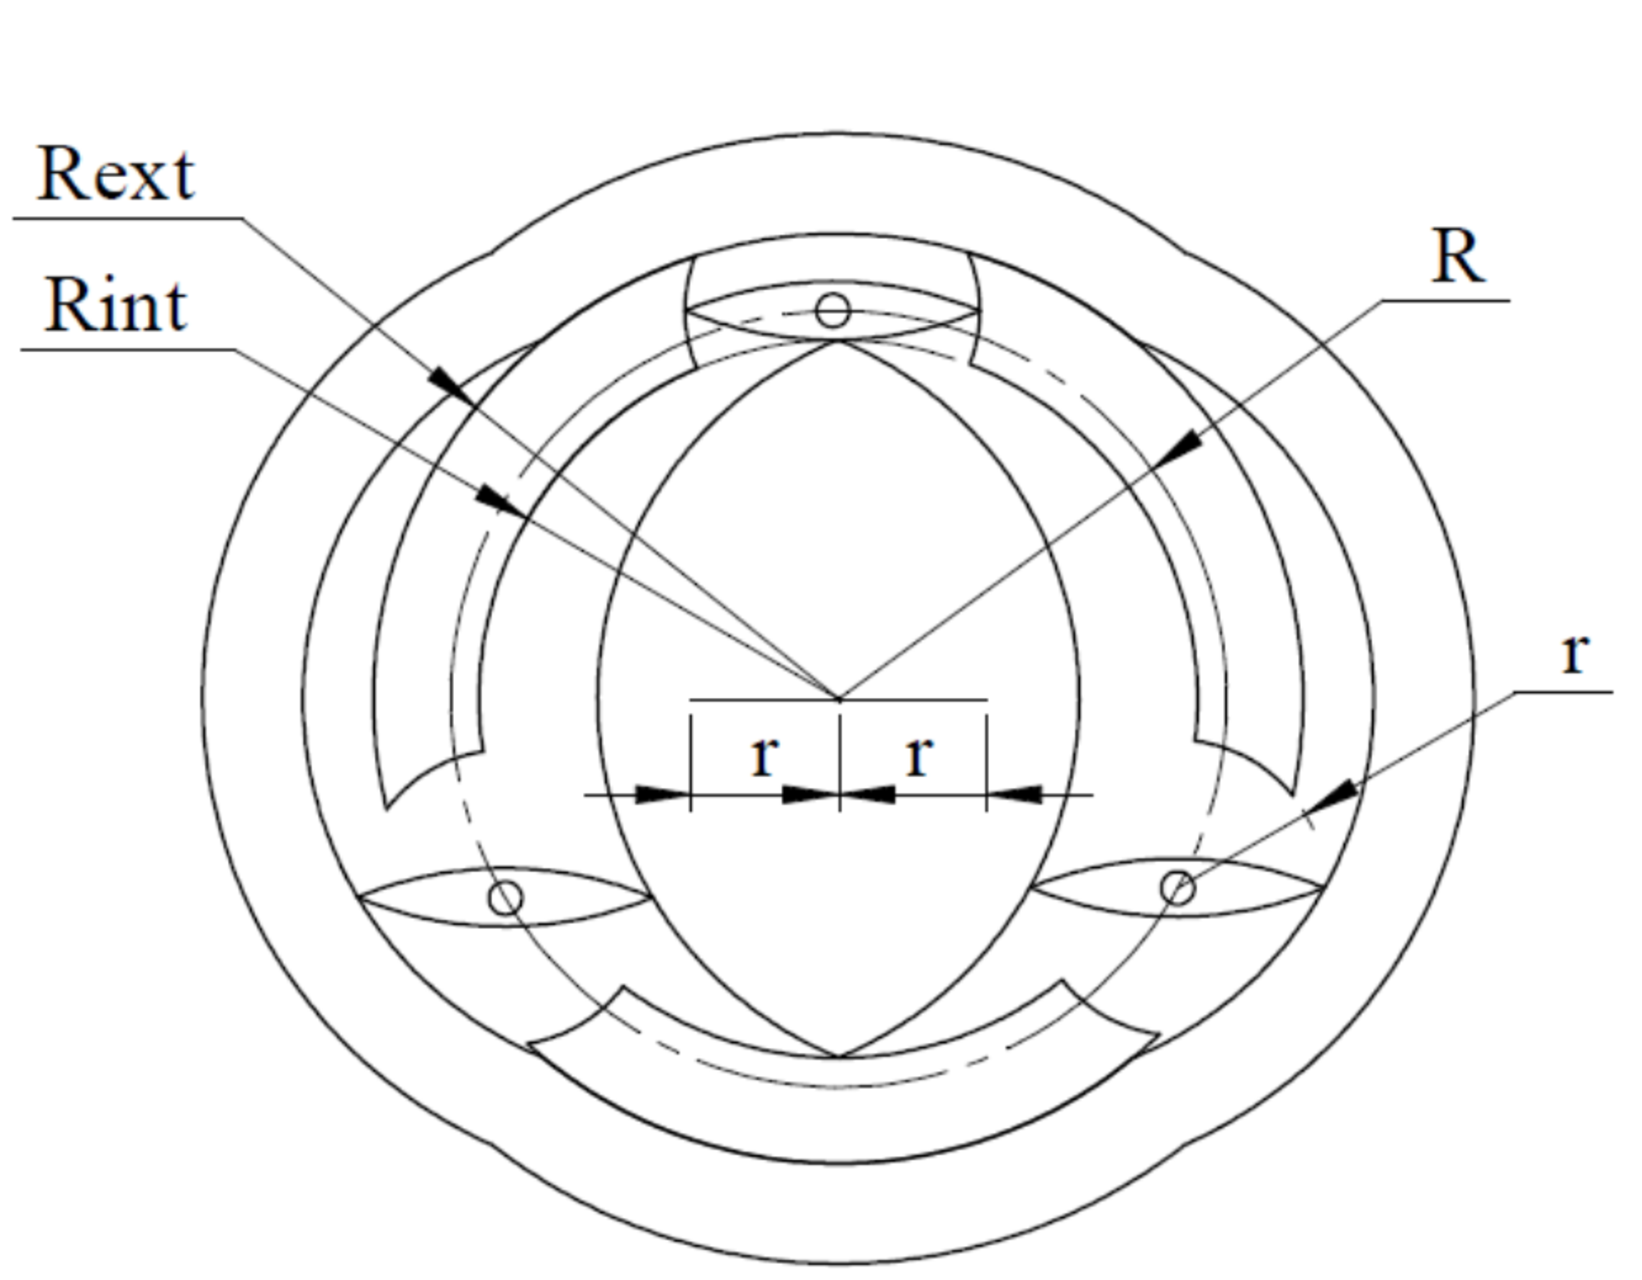
\includegraphics[width=0.7\textwidth]{plano_mrcvc_flor.pdf}
  \caption{Parámetros geométricos del MRCVC~\parencite{roldan20}}\label{fig:geom_flor_mrcvc}
\end{figure}

\begin{figure}[h!]
  \centering
  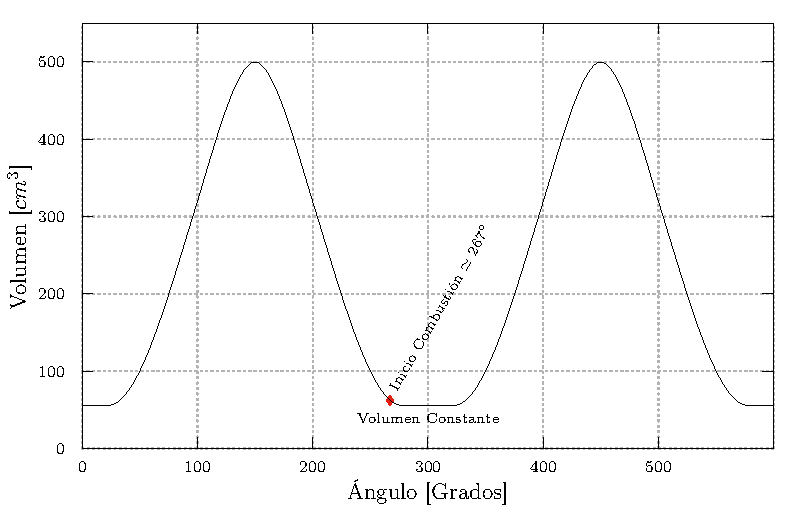
\includegraphics[width=0.7\textwidth]{gnuplot/vol.pdf}
  \caption{Variación del volumen del MRCVC}\label{fig:mrcvc_vol_cte}
\end{figure}

\begin{figure}[h!]
  \centering
  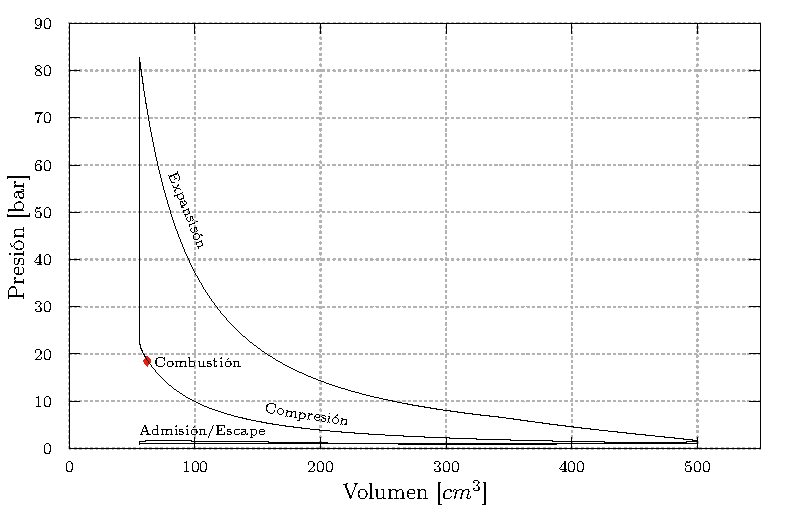
\includegraphics[width=0.7\textwidth]{gnuplot/vol_vs_pres.pdf}
  \caption{Ciclo operativo del MRCVC}\label{fig:PV_mrcvc}
\end{figure}

El ciclo operativo ideal del MRCVC es considerado un ciclo Otto en el que las
carreras de admisión, compresión, expansión y escape ocurren a medida que el
fluido de trabajo rota con respecto al eje del cigüeñal.
%
En la Figura~\ref{fig:ciclo_mrcvc} se puede ver una progresiva del ciclo del
MRCVC con estas carreras representadas en azul para la admisión, compresión en
amarillo, expansión en rojo y escape o barrido en violeta.

Durante el ciclo se destaca un aspecto particular de este motor, siguiendo la
paleta de color negro se ve que durante el proceso de compresión y combustión,
las paletas que forman la frontera aguas arriba y aguas abajo de la cámara de
combustión cambian.
%
La paleta que delimita el frente de la cámara se adelanta con respecto a la
cámara con la que inició el ciclo, produciendo que este dure más de una
revolución resultando en $600^{\circ}$ de giro del cigüeñal para el caso de 3
paletas considerado en este trabajo.

Para un motor con las características geométricas indicadas en la
Tabla~\ref{tab:geom_mrcvc}, el volumen mínimo alcanzado permanece constante por
un período de $\sim 44,65^\circ$, como se puede ver en la
Figura~\ref{fig:mrcvc_vol_cte} en donde se representa la variación del volumen
con respecto al ángulo de eje.
%
En este gráfico se indica el ángulo de inicio de la combustión, el cual
\emph{es una estimación} basada en datos de otros motores como
$\theta_{0}\simeq 267^{\circ}$.
%
En la Tabla se listan el número de paletas $n$, los radios $R$, $R_{e}$, $R_{i}$
y $r$, altura de cámara $h_{c}$, altura de puerto $h_{p}$ y relación de
compresión $r_{c}$

\begin{figure}[h!]
  \centering
  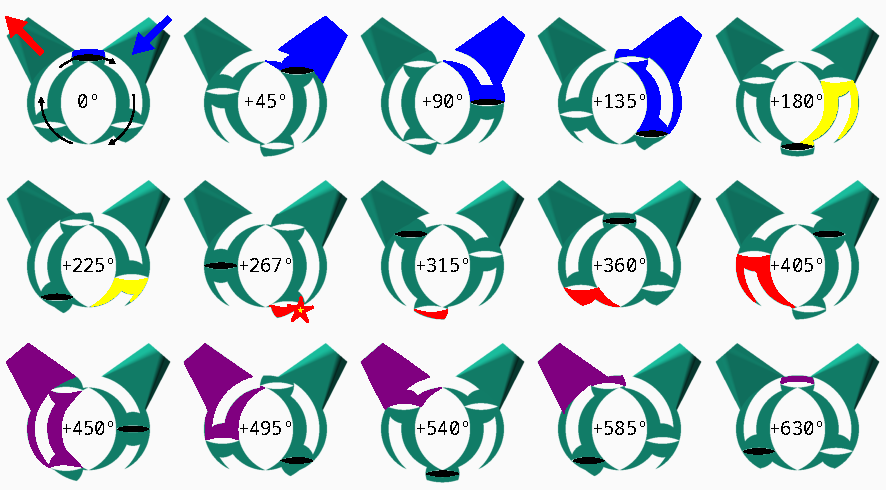
\includegraphics[width=\textwidth]{ciclo/ciclo_operativo.pdf}
  \caption{Ciclo operativo del MRCVC}\label{fig:ciclo_mrcvc}
\end{figure}

\begin{table}[h!]
    \centering
    \begin{tabular}{rccccccccc} \toprule
        Parámetro & n & R & r & $h_{c}$ & $h_{p}$ & rc & $V_{max}$ & $R_i$ & $R_e$ \\ \midrule
      Valor & 3 & 116.1 & 44.1 & 44.1 & 29.4 & 9 & 500 & 107.4 & 139.0 \\
     Unidades & --- & mm & mm & mm & mm & --- & $cm^3$ & mm & mm \\ \bottomrule
    \end{tabular}
    \caption{Datos de la geometría del MRCVC considerados en el trabajo}\label{tab:geom_mrcvc}
\end{table}

\nomenclature[G]{\(R\)}{Radio de referencia del MRCVC, ver Figura \ref{fig:mrcvc_vol_cte}}
\nomenclature[G]{\(R_{i}\)}{Radio de cara interna del rotor del MRCVC, ver Figura \ref{fig:mrcvc_vol_cte}}
\nomenclature[G]{\(R_{e}\)}{Radio de cara externa del rotor del MRCVC, ver Figura \ref{fig:mrcvc_vol_cte}}
\nomenclature[G]{\(r\)}{Radio de trayectoria de paletas, ver Figura \ref{fig:mrcvc_vol_cte}}
\nomenclature[G]{\(n\)}{Número de paletas del MRCVC}
\nomenclature[G]{\(h_c\)}{Altura de cámara}
\nomenclature[G]{\(h_p\)}{Altura de puerto}


%%%%%%%%%%%%%%%%%%%%%%%%%%%%%%%%%%%%%%%%%%%%%%%%%%%%%%%%%%%%%%%%%%%%%%%%%%%%%%%

\subsection{Sistemas de Intercambio de Gases}
%
En un motor típico de combustión interna de encendido por chispa, el sistema de
intercambio de gases se compone de una toma de aire, filtro, cuerpo de
mariposa, conducto y puerto de admisión, conducto y puerto de escape,
catalizador y silenciador hasta finalmente descargar en la atmósfera.

Para simplificar el sistema analizado no se tuvieron en cuenta elementos como:
mariposa, carburador, filtros de aire, convertidores catalíticos y demás; se
utilizó un sistema simplificado en el que solamente se tiene conducto de
admisión y escape junto con puertos de admisión y escape.
%
El eje de los conductos coincide con el eje del puerto, estos últimos hacen una
transición desde el diámetro del conducto hasta la altura de la ranura del
puerto en la cámara de combustión.
%
En la Figura~\ref{fig:sistema_intercambio_gases} se esquematiza la geometría
mencionada.

\begin{figure}[h!]
    \centering
    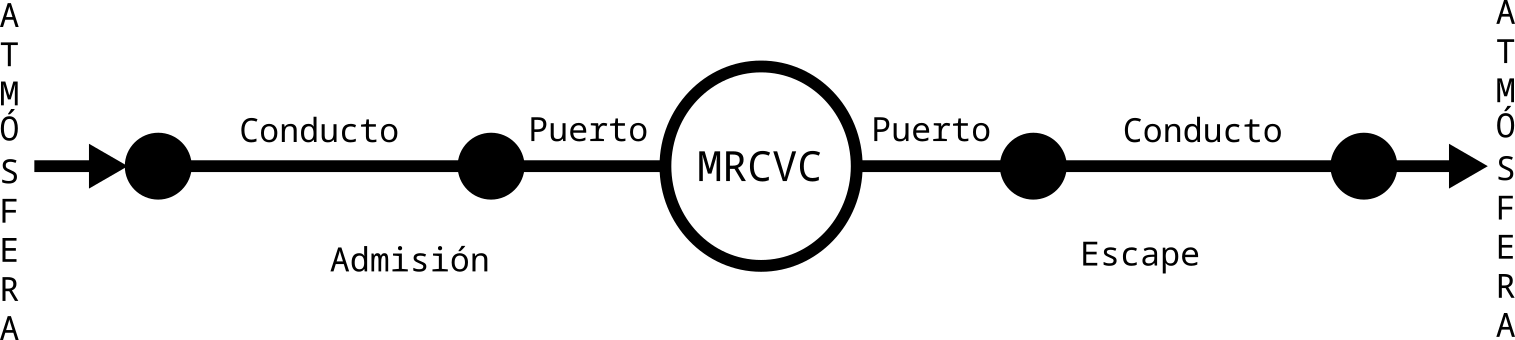
\includegraphics[width=\textwidth]{ciclo/sistema_intercambio_gases.png}
    \caption{Esquema del sistema de intercambio de gases}\label{fig:sistema_intercambio_gases}
\end{figure}


En trabajos anteriores~\parencite{lopez13} se demostró que se tiene una mejor
\emph{performance} del motor si se ubican los puertos en el cuerpo central del
estator, comparado al rendimiento obtenido con los puertos ubicados en las
tapas del mismo.
%
En dicho trabajo se realizó una optimización de la geometría mediante un
barrido paramétrico de las variables que determinan la forma, posición y
reglaje de los puertos, ya que es la ubicación angular de los puertos la que
determina la duración de los procesos de admisión y escape.
%
Los puertos están fijos en la periferia del estator y su posición se define con
los ángulos \emph{IIA}, \emph{IFA} para la admisión y \emph{EIA}, \emph{EFA}
para el escape, ver Figura~\ref{fig:angulos_puertos}.

\nomenclature[G]{\(IIA\)}{Ángulo de apertura del puerto de admisión, ver Figura \ref{fig:angulos_puertos}}
\nomenclature[G]{\(IFA\)}{Ángulo de cierre del puerto de admisión, ver Figura \ref{fig:angulos_puertos}}
\nomenclature[G]{\(EIA\)}{Ángulo de apertura del puerto de escape, ver Figura \ref{fig:angulos_puertos}}
\nomenclature[G]{\(EFA\)}{Ángulo de cierre del puerto de escape, ver Figura \ref{fig:angulos_puertos}}

\begin{figure}[h]
    \centering
    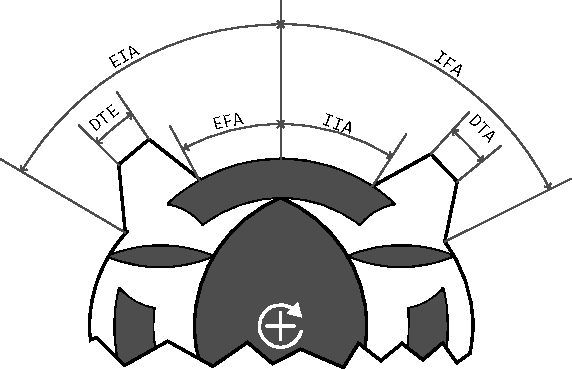
\includegraphics[width=0.6\textwidth]{/CAD/angulos.pdf}
    \caption{Puerto de admisión y escape}\label{fig:angulos_puertos}
\end{figure}

\begin{figure}[h]
\centering
  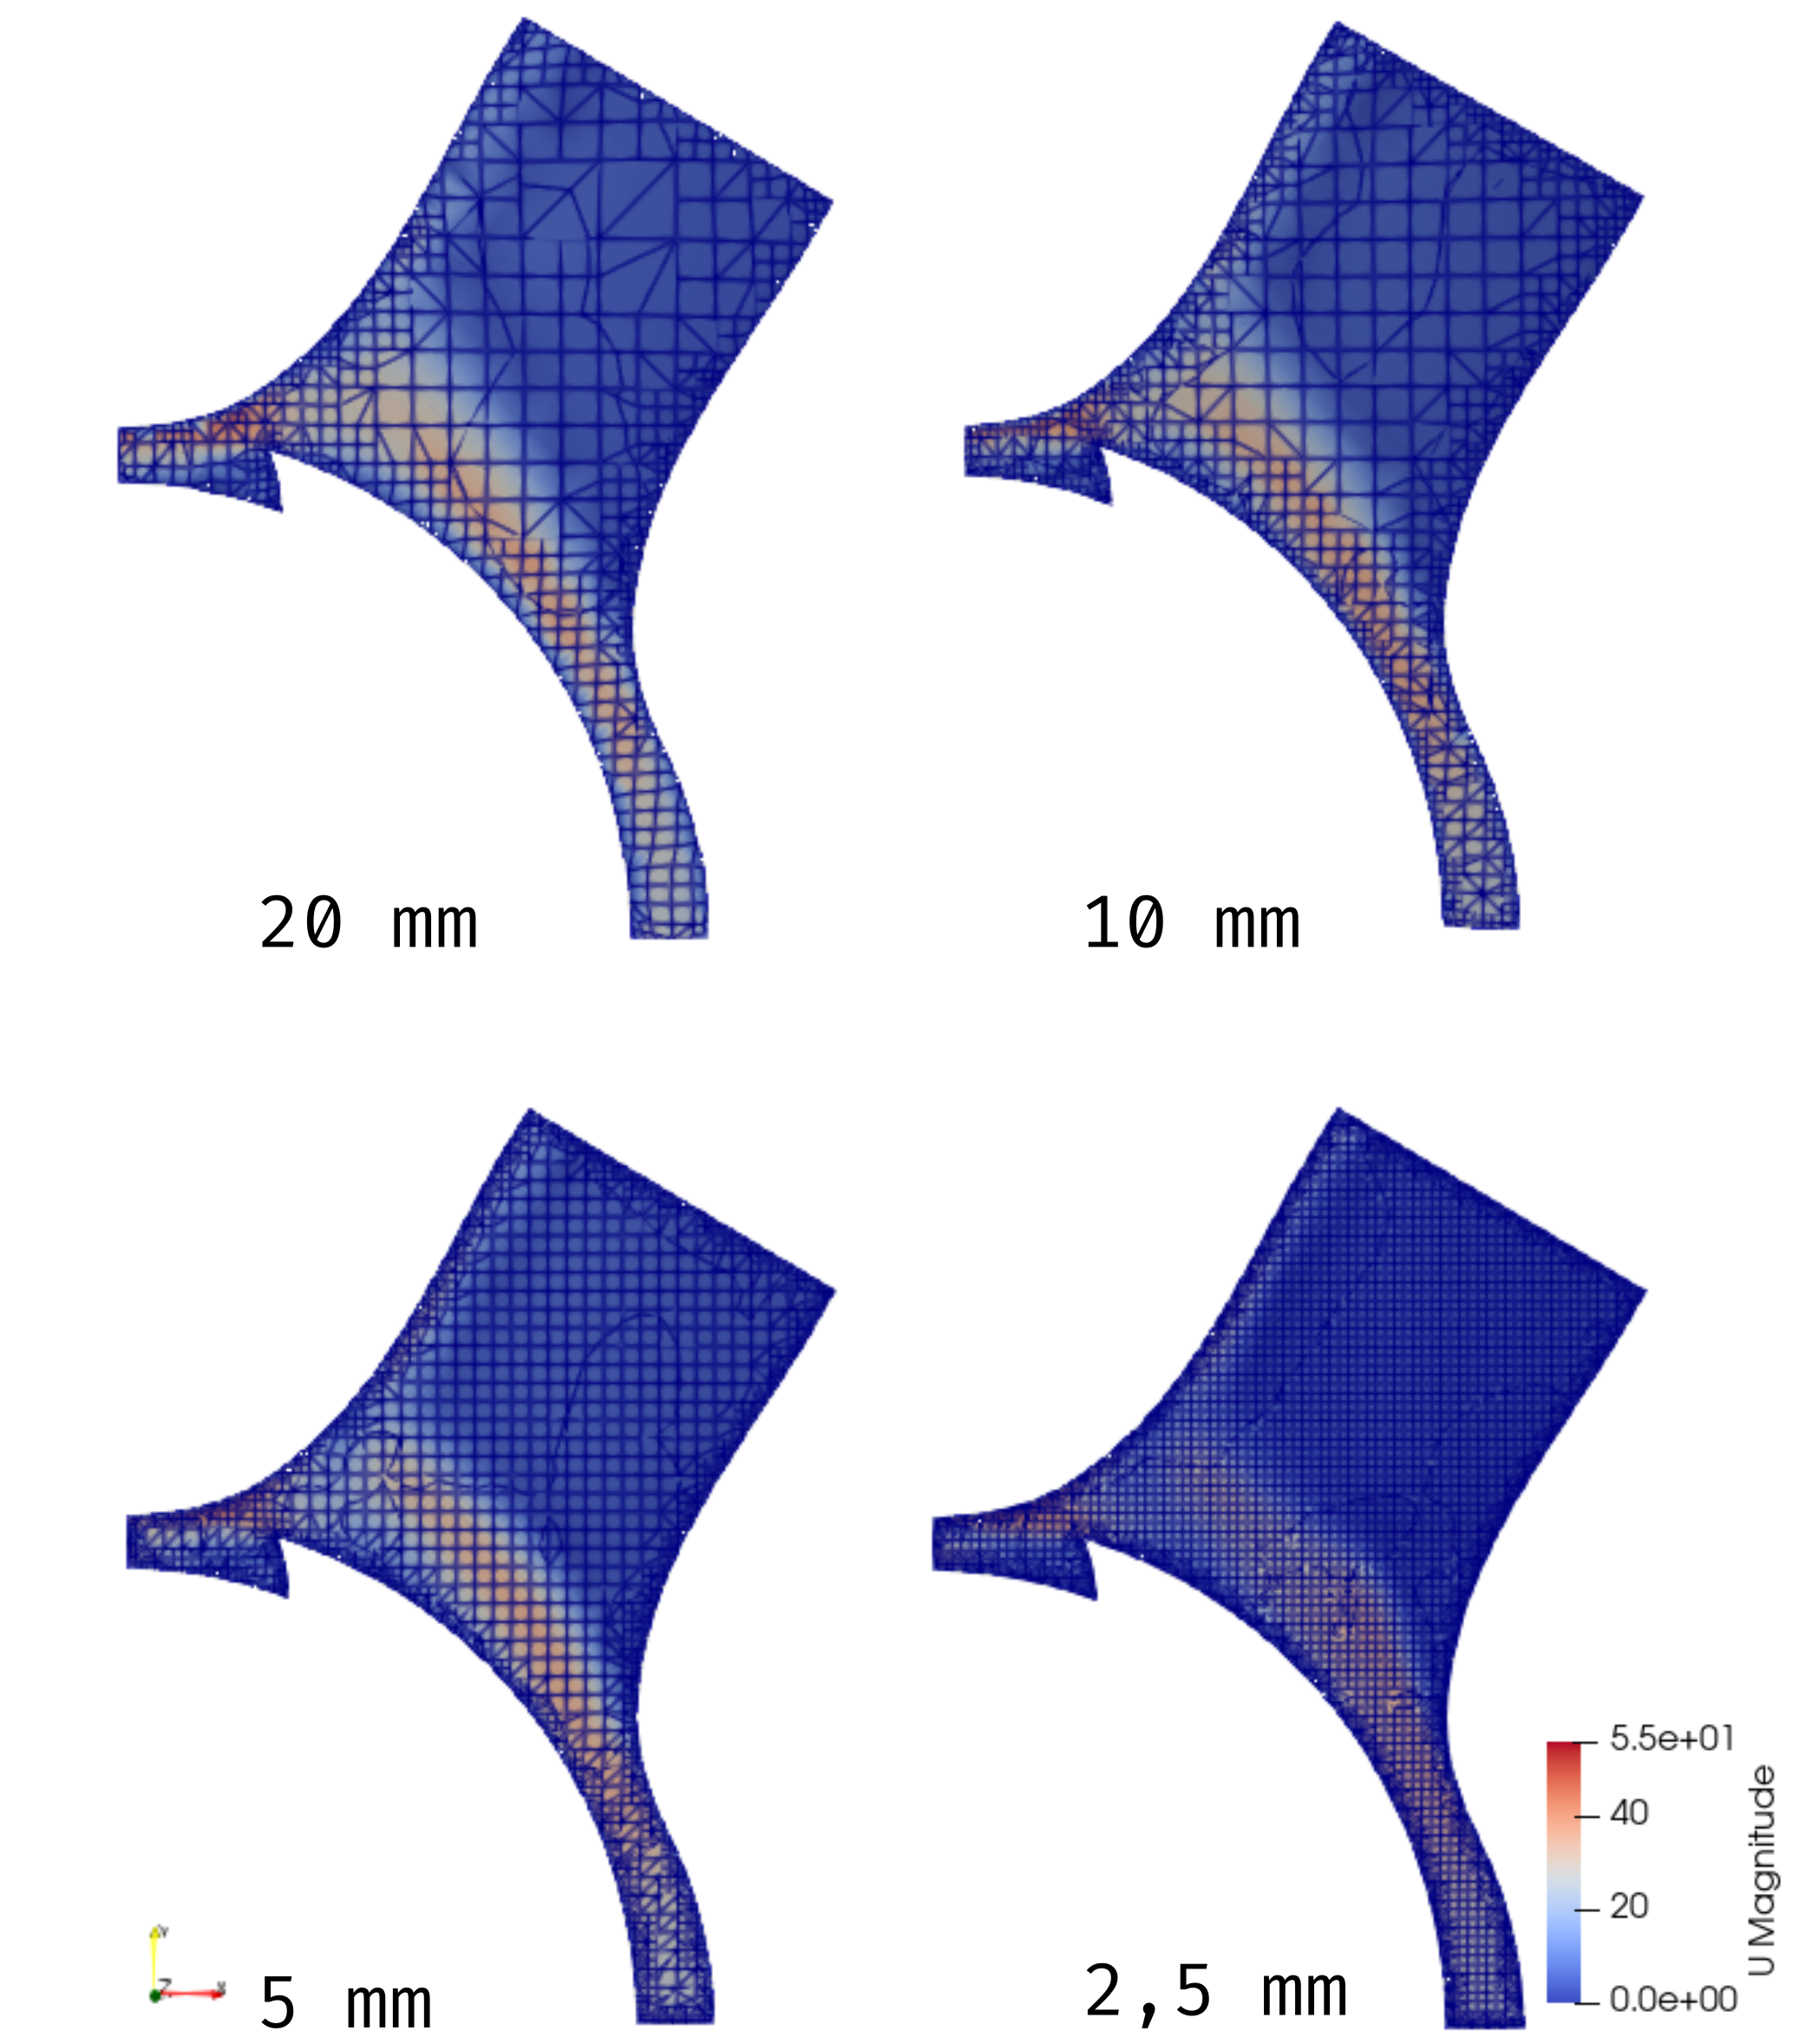
\includegraphics[]{./flujometrias/refinamiento_malla_admision.png}
  \caption{Refinamiento de malla para puerto de admisión}\label{fig:refinamiento_admision}
\end{figure}

\begin{figure}[h]
  \centering
  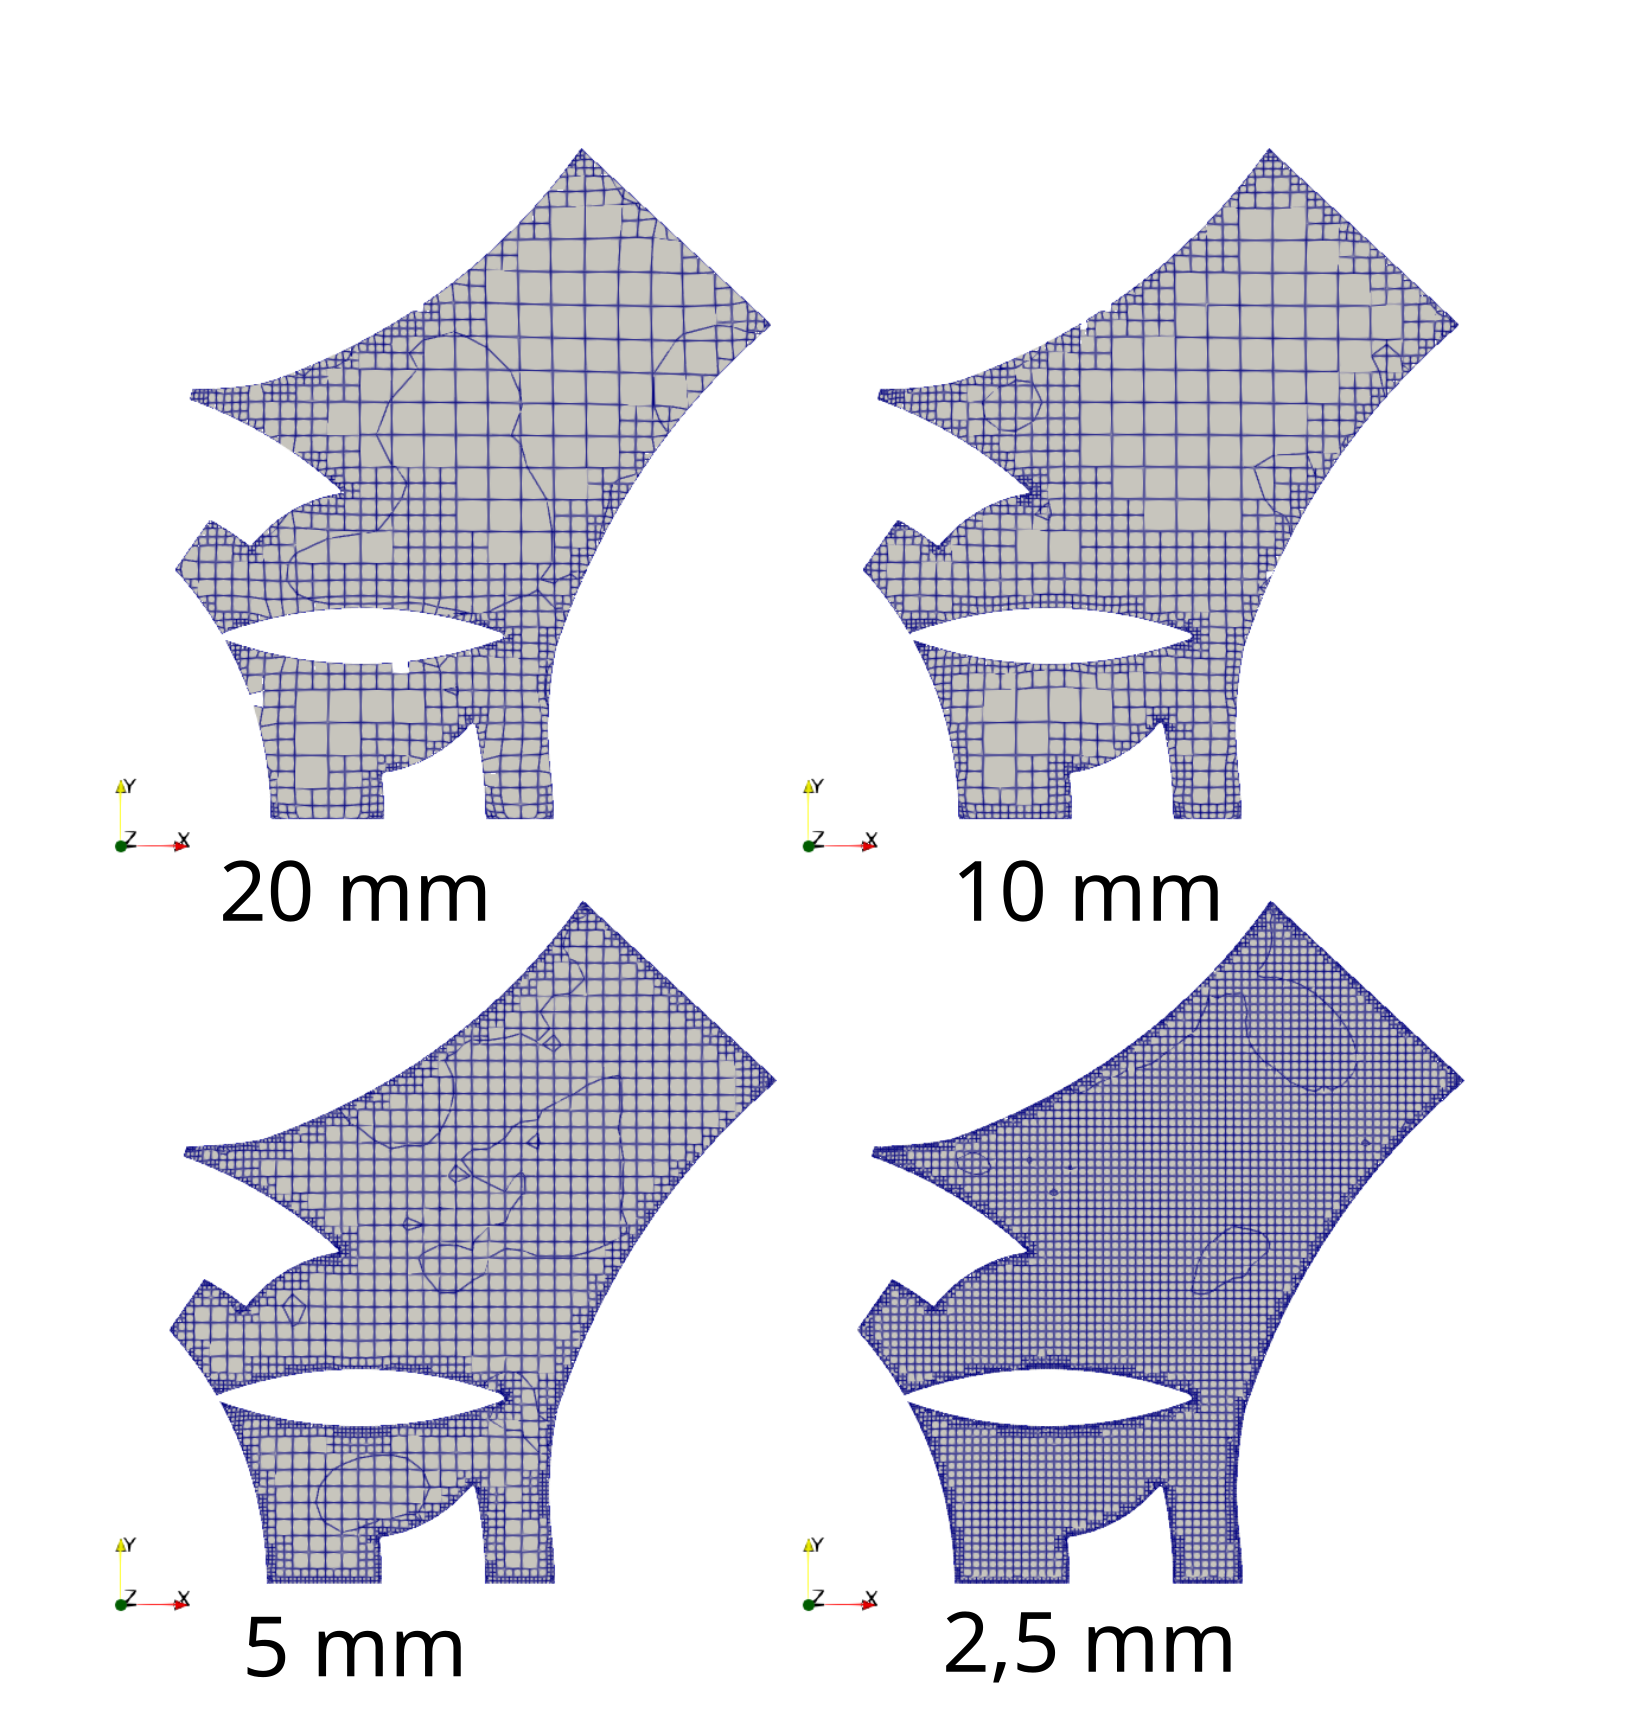
\includegraphics[]{./flujometrias/refinamiento_malla_escape.png}
  \caption{Refinamiento de malla para puerto de escape}\label{fig:refinamiento_escape}
\end{figure}

\begin{figure}[h]
  \centering
  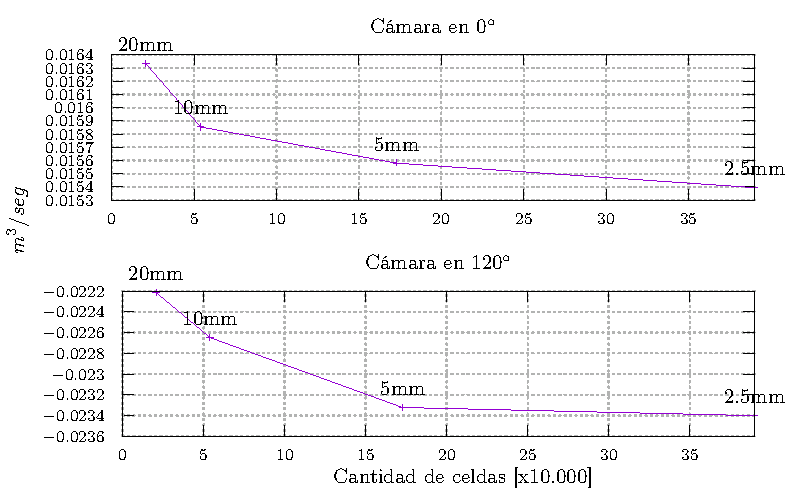
\includegraphics[width=0.9\textwidth]{./flujometrias/convergencia_admision_2000rpm.pdf}
  \caption{Convergencia de malla de puerto de admisión}\label{fig:conv_malla_admision}
\end{figure}

\begin{figure}[h]
  \centering
  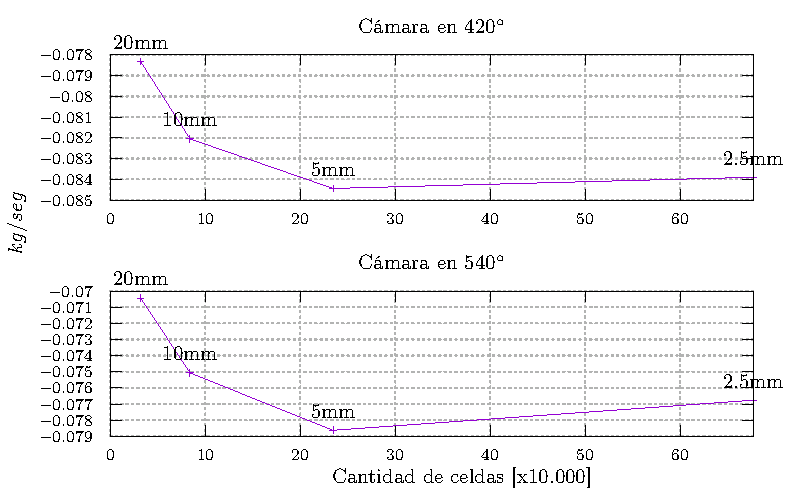
\includegraphics[width=0.9\textwidth]{./flujometrias/convergencia_escape_4000rpm.pdf}
  \caption{Convergencia de malla de puerto de escape}\label{fig:conv_malla_escape}
\end{figure}


Para este trabajo se realizaron las siguientes consideraciones:

\begin{enumerate}
        %
    \item El combustible utilizado es isooctano, la mezcla aire-combustible es
estequiométrica ($\phi=1$).
        %
    \item El sistema de intercambio de gases del MRCVC se compone de un conducto
y puerto admisión, conducto y puerto de escape.
        %
        ICESym tiene en cuenta pérdidas por fricción viscosa en los conductos,
los puertos generan pérdidas localizadas.
        %
    \item Los conductos se asumen como elementos rectos de un largo finito y
diámetro constante, cuya fuente y sumidero es la atmósfera a $101330 Pa$ y
$25^{\circ}C$.
        %
    \item La temperatura de la pared de la cámara de combustión se asume en
450K.
        %
    \item El motor es naturalmente aspirado.
        %
\end{enumerate}
%
\nomenclature[PO]{\(\phi\)}{Relación de equivalencia combustible/aire}

En la simulación del MRCVC se utilizó una mezcla estequiométrica de
aire-isooctano ($C_{8}H_{18}$) cuya reacción se indica en la
ecuación~(\ref{eq:estequeometrica}).

\begin{equation} \label{eq:estequeometrica}
  C_{8}H_{18} + 12,5 \left(O_{2}+3,772N_{2}\right) \rightarrow 8 CO_{2} + 9 H_{2}O + 47,16 N_{2}
\end{equation}

Expresando el combustible en función de la cantidad de moles de carbono,
$CH_{y}$ con $y=\frac{b}{a}=18/8=2.25$, se puede expresar la proporción
estequiométrica de aire combustible que se requiere con la
ecuación~(\ref{eq:rel_as}):

\begin{equation} \label{eq:rel_as}
  \left(\frac{A}{F}\right)_{s} = \left(\frac{F}{A}\right)_{s}^{-1} = \frac{34,56(4+2.25)}{12,011 + 1,008\cdot 2.25} \simeq 15.127
\end{equation}

\subsection{Área de Referencia}
%
Para el área de referencia ($A_{R}$) se utilizó el área frontal del puerto
expuesta a la cámara, la cual se obtiene del producto de la altura del puerto
$h_{p}$ y la distancia entre una arista del puerto y el extremo de la paleta
(eq.\ref{eq:ar_mrcvc}).
%
La altura de puerto vale $h_{p}=29,4$ mm.

\begin{equation}\label{eq:ar_mrcvc} 
    A_{R,i} = h_{p} \cdot l_{v,i}
\end{equation}

El área de utilizada se ilustra en la Figura~\ref{fig:area_referencia}.
%
Se observan dos zonas coloreadas que hacen referencia al área de dos cámaras
contiguas durante un período de solape de cámaras.


\begin{figure}[h]
  \centering
  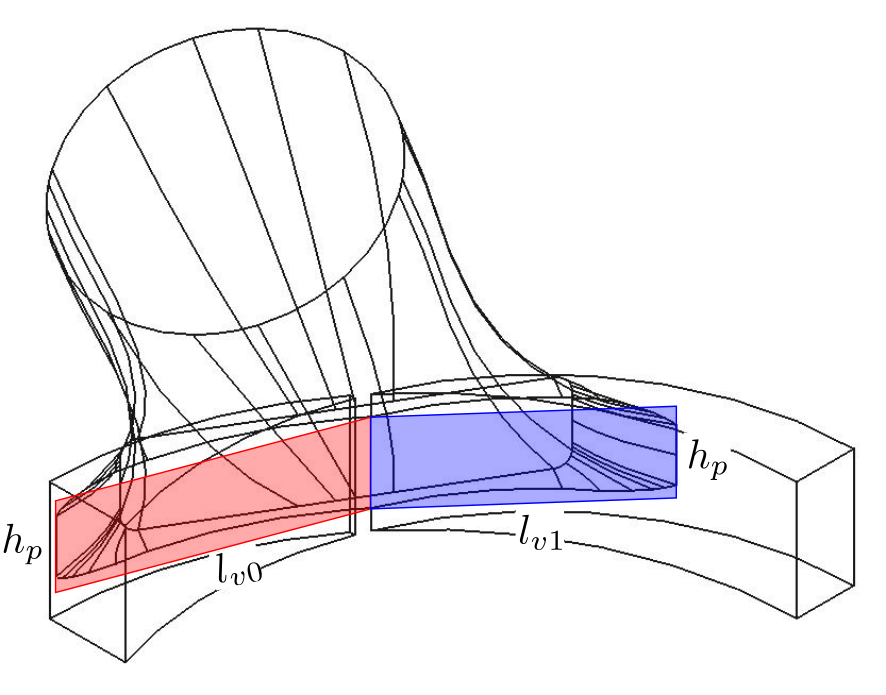
\includegraphics[width=.6\textwidth]{area_referencia.png}
  \caption{Área de referencia MRCVC}\label{fig:area_referencia}
\end{figure}

\subsection{Pérdidas por fricción}

Se incorporaron las pérdidas por rozamiento los sellos de las paletas y sellos
estatóricos del MRCVC utilizando valores obtenidos en trabajos
anteriores~\parencite{roldan20}.
%
El trabajo de fricción para diferentes velocidades se consideró en la etapa de
post-procesamiento de las simulaciones de ICESym.

La presión media efectiva de fricción (\textit{fmep}) se obtiene a partir del
trabajo de fricción y el volumen desplazado.

\begin{equation}
  fmep_{cilindro} = \frac{W_{f}}{V_{d}}
\end{equation}

En la Tabla~\ref{tab:trabajo_fricción} se presentan los valores de trabajo de
fricción correspondientes a diferentes regímenes velocidad.

\begin{table}[h!]
  \centering
  \begin{tabular}{cccccccccc}
    \toprule
    \textbf{RPM} & 1000 & 2000 & 3000 & 4000 & 5000 & 6000 & 7000 & 8000 & 9000 \\
    \midrule
    \textbf{$W_{f}$ [J]} & 25.204 & 26.19 & 26.619 & 27.755 & 28.781 & 31.392 & 28.449 & 31.975 & 32.263 \\
    \bottomrule
  \end{tabular}
  \caption{Pérdidas por fricción en sellos de paletas y sellos estatóricos}\label{tab:trabajo_fricción}
\end{table}



\section{Flujometrías Virtuales}
%
Se realizaron una serie de flujometrías para obtener valores de $C_{D}$ en
función de la diferencia de presión a través del puerto y la apertura del
mismo\footnote{ICESym utiliza alzada, por lo que se traduce área de pasaje de
puerto en alzada de válvula equivalente.}, con el fin de obtener un mapa del
coeficiente de descarga en función de la presión y apertura del puerto
($C_{D} = f(\Delta P,l_v)$).
%
ICESym requiere de información del $C_{D}$ para calcular el área efectiva
de pasaje de flujo de las válvulas (o puertos en el caso del MRCVC).
%
Introduciendo el mapa de $C_{D}$ se tiene un mejor modelado del funcionamiento
del sistema de intercambio de gases porque se conoce la pérdida de carga
localizada para un rango de operación del motor.

Para las flujometrías se utilizó el software OpenFOAM seleccionando el algoritmo
PIMPLE, con sus implementaciones ``pimpleFoam'' y ``rhoPimpleFoam'' para los
casos en los que se considera un fluido de trabajo incompresible y compresible
respectivamente.
%
La configuración del software se detalla en la Sección~\ref{sec:3_openfoam}.

\subsection{Modelos de Turbulencia}
%
El flujo a través del puerto es de carácter transitorio, turbulento.
%
Para modelar este tipo de flujo se utilizó el modelo de turbulencia de dos
ecuaciones \emph{$\kappa-\epsilon$}\parencite{wilcox}, que consta de una
ecuación para la \emph{energía cinética turbulenta} $\kappa$ y otra para la
\emph{tasa de disipación de la energía cinética turbulenta} $\epsilon$.
%
El modelo está basado en el modelo estándar
$\kappa-\epsilon$~\parencite{launderSpalding} y es uno de los más populares con
\emph{performance} conocida.
%
Las ecuaciones del modelo son:

\begin{equation}\label{eq:k}
  \frac{D}{Dt}(\rho \kappa) = \nabla \cdot (\rho D_{\kappa}\nabla \kappa) + P_{\kappa} - \rho \epsilon
\end{equation}

\nomenclature[PO]{\(\rho\)}{Densidad}
\nomenclature[F]{\(\kappa\)}{Energía cinética turbulenta}
\nomenclature[F]{\(D_{\kappa}\)}{Difusividad efectiva para $\kappa$}
\nomenclature[F]{\(P_{\kappa}\)}{Tasa de producción de energía cinética turbulenta}
\nomenclature[F]{\(\epsilon\)}{Tasa de disipación de energía cinética turbulenta}

donde

\begin{itemize}
  \item[-] $\kappa$ es la energía cinética turbulenta.
  \item[-] $D_{\kappa}$ es la difusividad efectiva para $\kappa$.
  \item[-] $P_{\kappa}$ es la tasa de producción de energía cinética turbulenta.
  \item[-] $\epsilon$ es la tasa de disipación de energía cinética turbulenta.
\end{itemize}


\begin{equation}\label{eq:k}
  \frac{D}{Dt}(\rho \epsilon) =
  \nabla \cdot (\rho D_{\epsilon}\nabla \epsilon) +
  \frac{C_{1}\epsilon}{\kappa} \left( P_{\kappa}+C_{3}\frac{2}{3}\kappa\nabla\cdot u \right) -
  C_{2}\rho\frac{\epsilon^{2}}{\kappa}
\end{equation}

donde
\begin{itemize}
  \item[-] $D_{\epsilon}$ es la difusividad efectiva de $\epsilon$.
  \item[-] $C_{1}$ es un coeficiente del modelo.
  \item[-] $C_{2}$ es un coeficiente del modelo.
\end{itemize}

La ecuación para la viscosidad turbulenta $\nu_{t}$ es

\begin{equation}\label{eq:nu_t}
  \nu_{t} = C_{\mu}\frac{\kappa^{2}}{\epsilon}
\end{equation}

\nomenclature[F]{\(\nu_{t}\)}{Viscosidad cinemática turbulenta}

donde
\begin{itemize}
        \item[-] $C_{\mu}$ es un coeficiente del modelo.
\end{itemize}

Los coeficientes por defecto del modelo son:

% Clossure Coefficient
\begin{equation}
  C_{\epsilon 1}=1,44
  \quad
  C_{\epsilon 2}=1,92
  \quad
  C_{\mu}=0,09
  \quad
  \sigma_{k}=1
  \quad
  \sigma_{\epsilon}=1,3
\end{equation}

El valor inicial para $\kappa$ se puede estimar con:
\begin{equation}\label{eq:kappa_est}
  \kappa = \frac{3}{2} {\left( |u_{ref}| \cdot I \right)}^{2}
\end{equation}

\nomenclature[F]{\(I\)}{Intensidad de turbulencia}

donde
\begin{itemize}
  \item[-] $I$ es la intensidad de turbulencia.
  \item[-] $u_{ref}$ es una velocidad de referencia en $ms^{-1}$.
\end{itemize}

El valor inicial para $\epsilon$ se puede estimar con:
\begin{equation}\label{eq:epsilon_est}
  \epsilon = \frac{{C_{\mu}}^{3/4} \cdot {\kappa}^{3/2}} {l_{m}}
\end{equation}

donde
\begin{itemize}
 \item[-] $l_{m}$ es una longitud de referencia, para flujos internos se estima
con el diámetro hidráulico de la cañería, usando por ejemplo $0,07 \cdot D_{m}$.
\end{itemize}

\nomenclature[F]{\(l_m\)}{Longitud de mezcla o escala de viscosidad}

% https://www.openfoam.com/documentation/guides/latest/doc/guide-turbulence-ras-k-epsilon.html

Las ecuaciones anteriores de  $\kappa$ y $\epsilon$ son estimaciones para dar un
valor inicial al problema.
%
La longitud de mezcla $l_m$ determina el tamaño que pueden tener los torbellinos
turbulentos, su valor inicial se aproximó como la altura de cámara $l_m = h_c$.
%
Esta estimación de $l_{m}$ a priori parece algo elevado, es un valor que se
utilizó para inicializar la simulación.


\subsection{Condiciones Iniciales}\label{cap2:cond_iniciales}
%
Las condiciones iniciales se determinan para diferentes puntos operativos de
interés del motor a partir de los datos obtenidos del simulador ICESym.
%
Se tienen dos casos distintivos al momento de modelar el flujo a través de los
puertos: flujo compresible e incompresible.
%
Para este último se considera que los efectos de la compresibilidad del gas se
pueden despreciar cuando el número de Mach es menor a $0,3$.
%
Cuanto mayor sea el número de Mach, mayor es el error que se comete por no
considerar los efectos de la compresibilidad en la simulación.
%
Además, se deben separar los casos a modelar entre aquellos en los que hay
solape de cámaras y los que no (ver Figura~\ref{fig:solape}).
%
En estos casos se define también un valor medio para inicializar el interior
del dominio que representa el gas dentro de la cámara.

\begin{figure}[t!]
  \centering
    \begin{subfigure}[t]{0.4\textwidth}
        \centering
        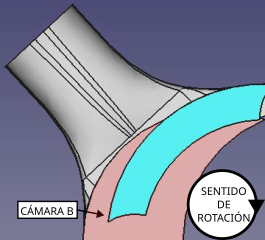
\includegraphics[width=\textwidth]{flujometrias/sin_solape.png}
        \caption{Sin solape}
    \end{subfigure}%
    \begin{subfigure}[t]{0.4\textwidth}
        \centering
        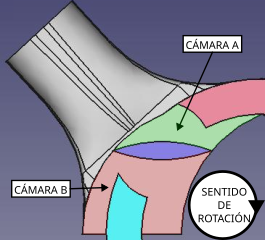
\includegraphics[width=\textwidth]{flujometrias/con_solape.png}
        \caption{Con solape}
    \end{subfigure}
  \caption{Solape de cámaras}\label{fig:solape}
\end{figure}

Independientemente del tipo de flujo que se esté simulando, de ICESym se toman
los valores de presión, temperatura, densidad y velocidad para calcular los
valores iniciales.

Debido a la cantidad de flujometrías a realizar, se utilizó un \emph{script}
para leer los datos de salida de ICESym y calcular los valores requeridos en
función del tipo de flujo a simular.
%
Este \emph{script} toma el estado del gas del simulador tanto en la cámara como
del puerto que se esté analizando, para la posición de alzada y RPM requeridas.
%
De la simulación con ICESym se leen los valores listados en la
Tabla~\ref{tab:valores_iniciales} a partir de los cuales se pueden calcular las
propiedades termodinámicas de la mezcla de gases frescos o quemados,
dependiendo si se está evaluando un puerto de admisión o escape.

Para simplificar el análisis no se tuvo en cuenta la fracción de gases
residuales, el gas ``flujado'' es siempre aire limpio en el caso de los puertos
de admisión o el gas quemado de una mezcla estequiométrica de aire-combustible
en caso de los puertos de escape, siendo isooctano $C_{8}H_{18}$ el combustible
seleccionado.
%
Las ecuaciones utilizadas para modelar las propiedades termodinámicas de las
mezclas aire-combustible fueron descritas brevemente en la
sección~\ref{subsec:prop_mezcla}.
%
Los valores calculados son los indicados en la
Tabla~\ref{tab:valores_calculados}.

\begin{table}[h!]
  \centering
  \begin{tabular}{cl}\toprule
    Símbolo & Descripción \\ \midrule
    $\rho_{c,i}$ & es la densidad del gas en la cámara $i$ \\
    $P_{c,i}$ & es la presión del gas en la cámara $i$ \\
    $T_{c,i}$ & es la temperatura del gas en la cámara $i$ \\
    $\rho_{p,i}$ & es la densidad del puerto $i$ \\
    $v_{p,i}$ & es la velocidad del gas en el puerto $i$ \\
    $P_{p,i}$ & es la presión del gas en el puerto $i$ \\ \bottomrule
  \end{tabular}
\caption{Valores iniciales}\label{tab:valores_iniciales}
\end{table}

\begin{table}[h!]
  \centering
  \begin{tabular}{cll}\toprule
    Símbolo & Descripción & Ecuación\\ \midrule
    $M_{M}$ & masa molar & \ref{eq:mw} \\
    $C_{p}$ & calor específico a presión constante & - \\
    $\gamma$ & relación $C_{p}/C_{v}$ del gas & - \\
    $\mu$ & viscosidad dinámica & \ref{eq:mu} \\
    $\nu$ & viscosidad cinemática & - \\
    $P_{R}$ & número de Prandtl & \ref{eq:pr} \\
    $k_{est}$ & energía cinética turbulenta & \ref{eq:kappa_est} \\
    $\epsilon_{est}$ & disipación de la energía cinética turbulenta & \ref{eq:epsilon_est} \\ \bottomrule
  \end{tabular}
  \caption{Valores calculados}\label{tab:valores_calculados}
\end{table}

\nomenclature[F]{\(M_{M}\)}{Masa molar}
% \nomenclature[F]{\(C_{p}\)}{Calor específico a presión constante}
\nomenclature[F]{\(\gamma\)}{Cociente de calores específicos}
\nomenclature[F]{\(\mu\)}{Viscosidad dinámica}
\nomenclature[F]{\(\nu\)}{Viscosidad cinemática}
\nomenclature[F]{\(P_{R}\)}{Número de Prandtl}
% \nomenclature[F]{\(k_{est}\)}{Energía cinética turbulenta}


\subsection{Malla}

La malla se construyó a partir del modelo de CAD generado con los resultados
obtenidos de las simulaciones del motor.
%
La implementación de las diferentes herramientas requeridas para generar una
malla apta para realizar las flujometrías se describe en el
apartado~\ref{sec:cap3_of_malla}.

El grado de refinamiento de la malla utilizada para modelar el dominio de la
flujometría tiene un impacto directo en la calidad de los resultados ya que
está relacionado con el error de discretización.
%
Por otro lado, mallas con un alto nivel de refinamiento implican un mayor costo
computacional y dado la cantidad de flujometrías que requiere el trabajo se
optó por determinar un nivel de refinamiento que devuleva una diferencia
relativa entre dos mallas consecutivas no mayor al $5\%$.

Para los puertos de admisión se seleccionó la geometría representada en la
Figura~\ref{fig:refinamiento_admision}.
%
En esta posición hay dos cámaras activas, una con el ciclo en $0^{\circ}$ y
otra a $120^{\circ}$.
%
Las condiciones iniciales se determinan a partir de datos del simulador con el
motor girando a 2000 RPM.%
%
Para los puertos de escape se seleccionó la geometría representada en la
Figura~\ref{fig:refinamiento_escape}.
%
Esta posición corresponde a un período de solape de los puertos con dos cámaras
activas ubicadas en $420^{\circ}$ y $540^{\circ}$.
%
Las condiciones inciales se determinan de los datos de ICESym con el motor
girando a 4000 RPM.

Ambos puertos se simularon con tamaños de malla iniciales de 20, 10, 5 y 2,5 mm,
evaluando la variación del caudal con la cantidad de celdas de la malla, ver
Figura~\ref{fig:refinamiento_admision} para el puerto de admisión y
Figura~\ref{fig:refinamiento_escape} para el puerto de escape.
%
En las Tablas~\ref{tab:convergencia_malla_admision}
y~\ref{tab:convergencia_malla_escape} se presentan los resultados de los
refinamientos junto con el error relativo entre refinamientos sucesivos.

No se observa gran diferencia entre los casos de 20mm a 2,5mm pese a que la
cantidad de celdas es más de 18 veces mayor.
%
Esto se debe a que el software utilizado para realizar el mallado se configuró
para realizar un refinamiento de todas las superficies y bordes, para captar la
geometría de los puertos.
%
En la Figura~\ref{fig:conv_malla_admision} o~\ref{fig:conv_malla_escape} se
puede apreciar la diferencia de tamaño entre las celdas cercanas a las paredes
del puerto y las celdas pertenecientes al interior del volumen para la malla
con tamaño inicial de 20mm.

\begin{table}[h!]
  \centering
  \begin{tabular}{cccccc}\toprule
    Tamaño de celda & $N^{\circ}$ Celdas & $Q_{0^{\circ}} [dm^{3}/seg]$ & $\varepsilon_{r,0^{\circ}}$ & $Q_{120^{\circ}} [cm^{3}/seg]$ & $\varepsilon_{r,120^{\circ}}$ \\ \midrule
    20mm  & 20680  & 16,335 & -        & -22,216 & - \\
    10mm  & 53948  & 15,855 & $3,03\%$ & -22,649 & $1,91\%$ \\
    5mm   & 172853 & 15,58  & $1,76\%$ & -23,323 & $2,89\%$ \\
    2,5mm & 389980 & 15,395 & $1,20\%$ & -23,401 & $0,34\%$ \\ \bottomrule
  \end{tabular}
  \caption{Figura~\ref{fig:conv_malla_admision} tabulada}\label{tab:convergencia_malla_admision}
\end{table}

\begin{table}[h!]
  \centering
  \begin{tabular}{cccccc}\toprule
    Tamaño de celda & $N^{\circ}$ Celdas & $\dot{m}_{420^{\circ}} [g/seg]$ & $\varepsilon_{r,420^{\circ}}$ & $\dot{m}_{540^{\circ}} [g/seg]$ & $\varepsilon_{r,540^{\circ}}$ \\ \midrule
    20mm  & 31933  & -78,325 & - & -70,43 & - \\
    10mm  & 83817  & -82,048 & 4,54\% & -75,075 & 6,19\% \\
    5mm   & 234487 & -84,44  & 2,83\% & -78,626 & 4,52\% \\
    2,5mm & 676850 & -83,897 & 0,65\% & -76,766 & 2,42\% \\ \bottomrule
  \end{tabular}
  \caption{Figura~\ref{fig:conv_malla_escape} tabulada}\label{tab:convergencia_malla_escape}
\end{table}

\begin{figure}[h]
  \centering
  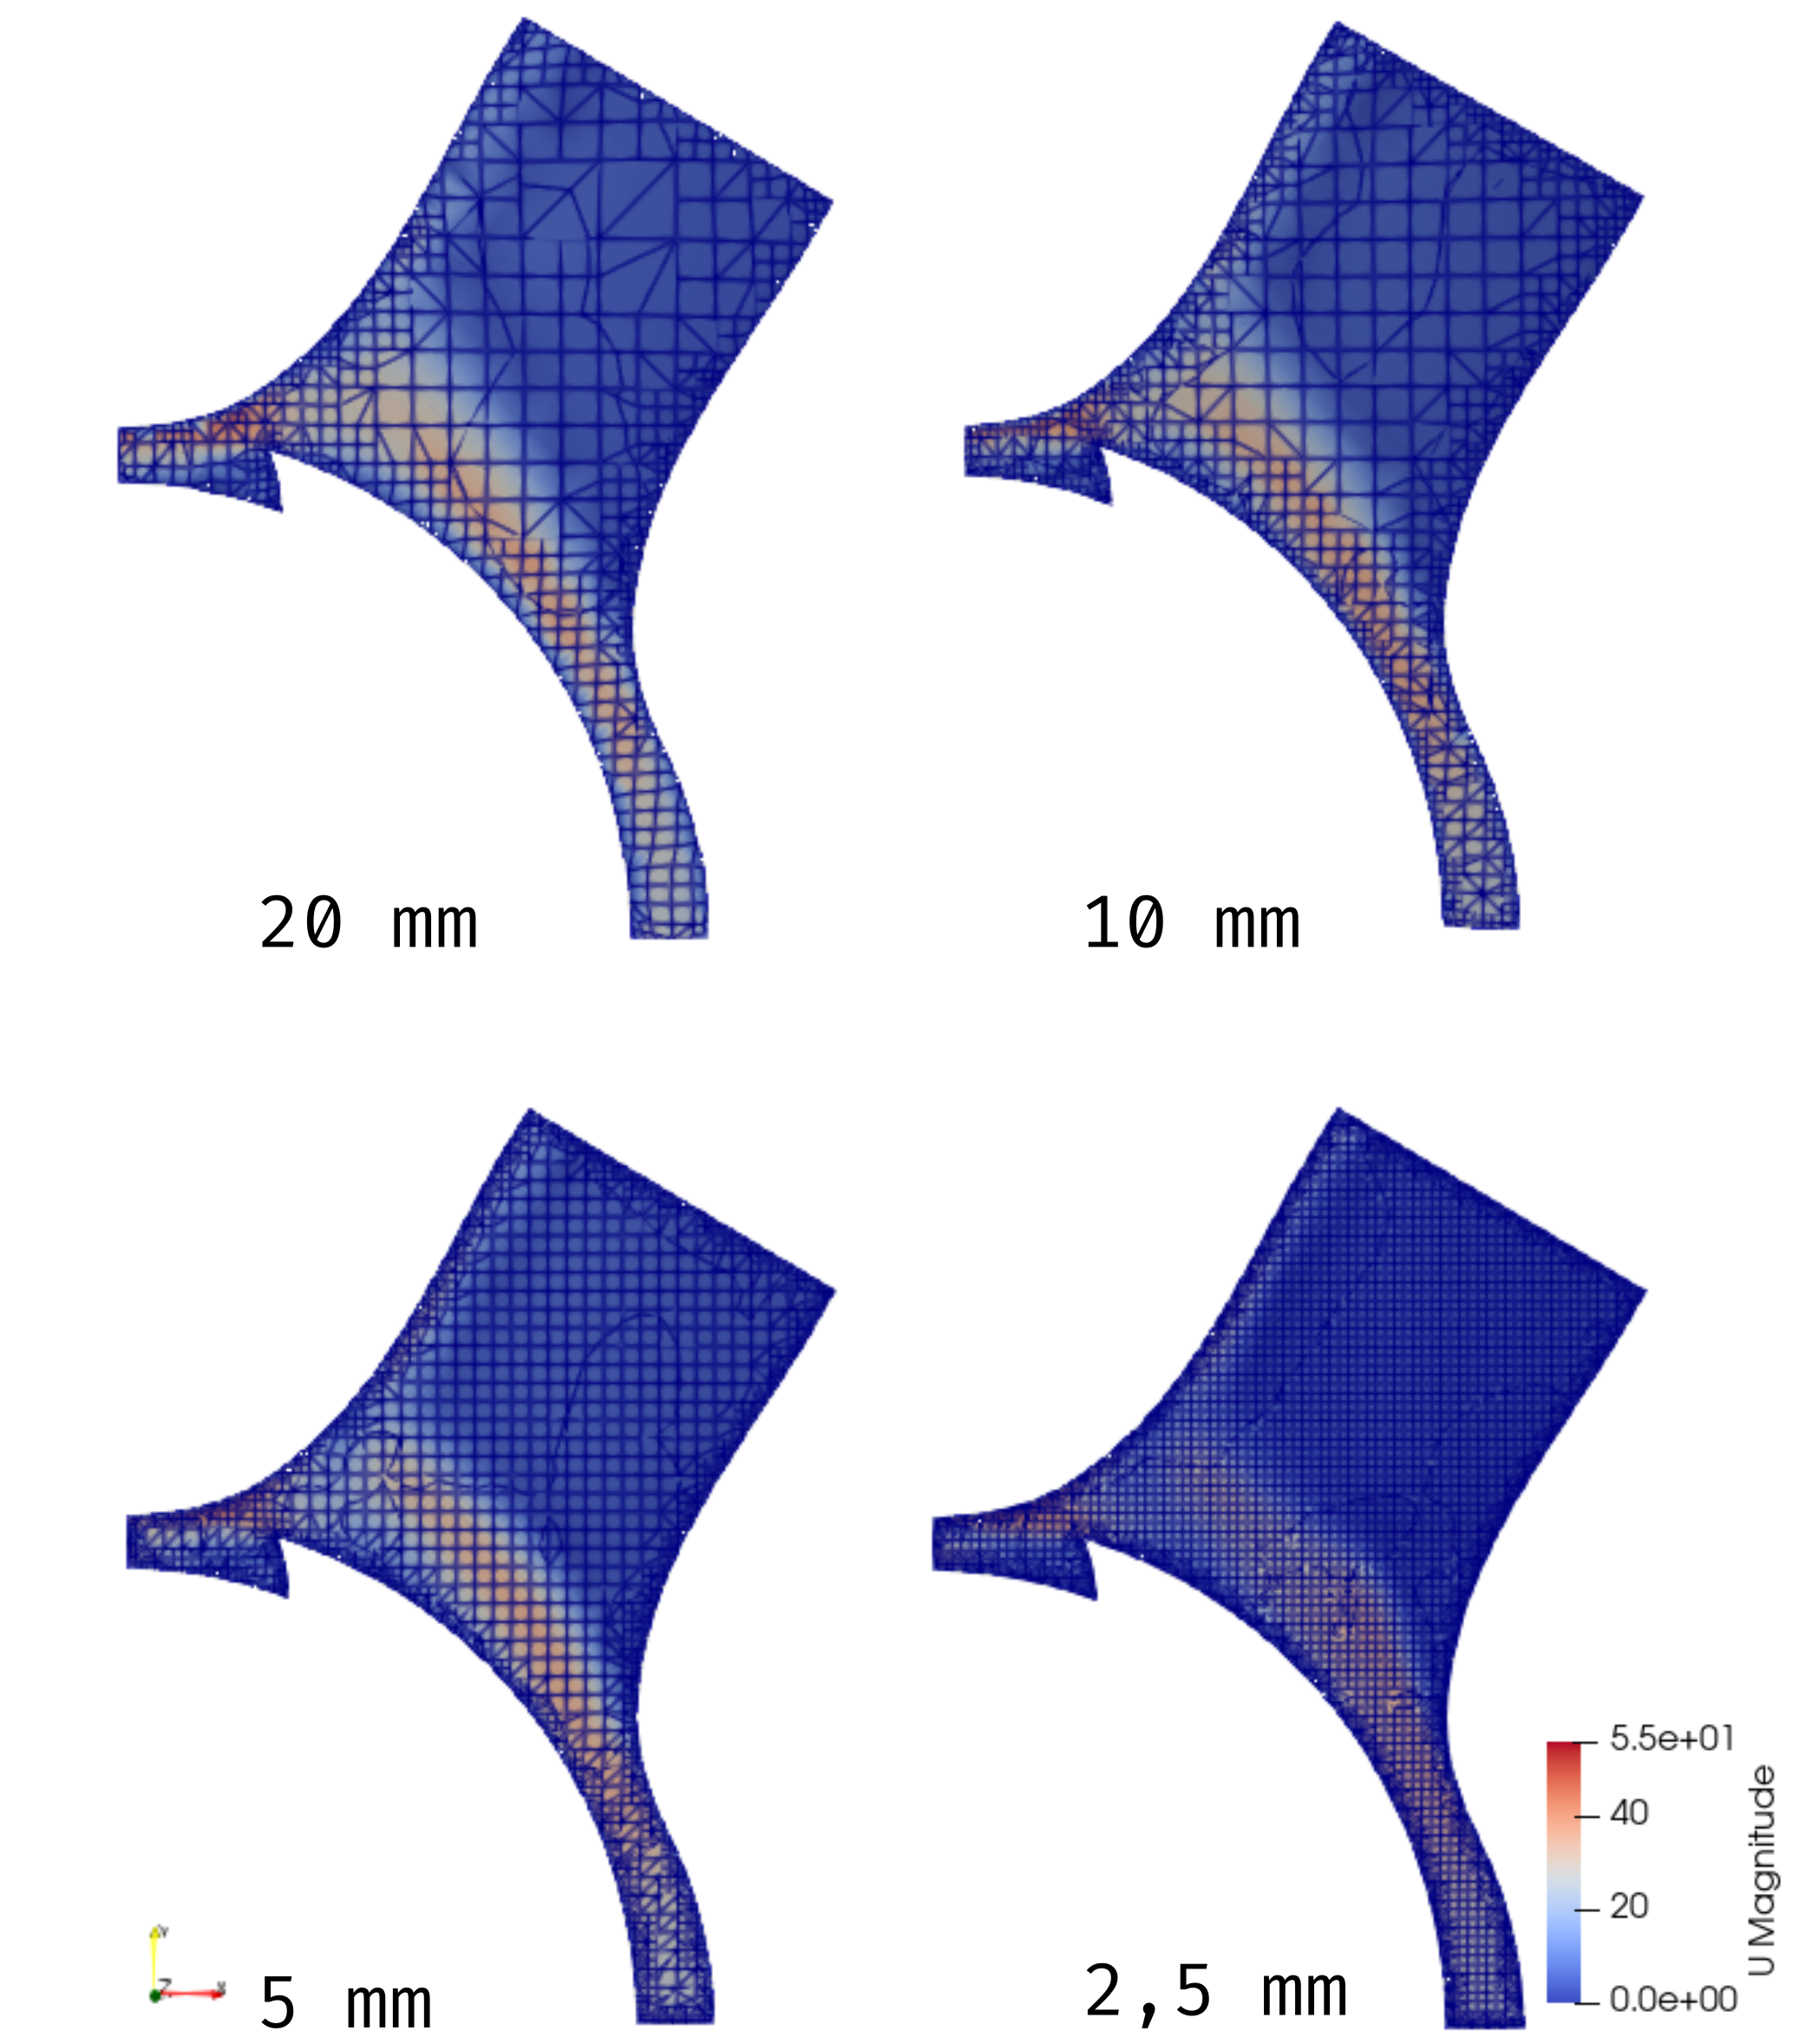
\includegraphics[width=0.8\textwidth]{./flujometrias/refinamiento_malla_admision.png}
  \caption{Refinamiento de malla para puerto de admisión}\label{fig:refinamiento_admision}
\end{figure}

\begin{figure}[h]
  \centering
  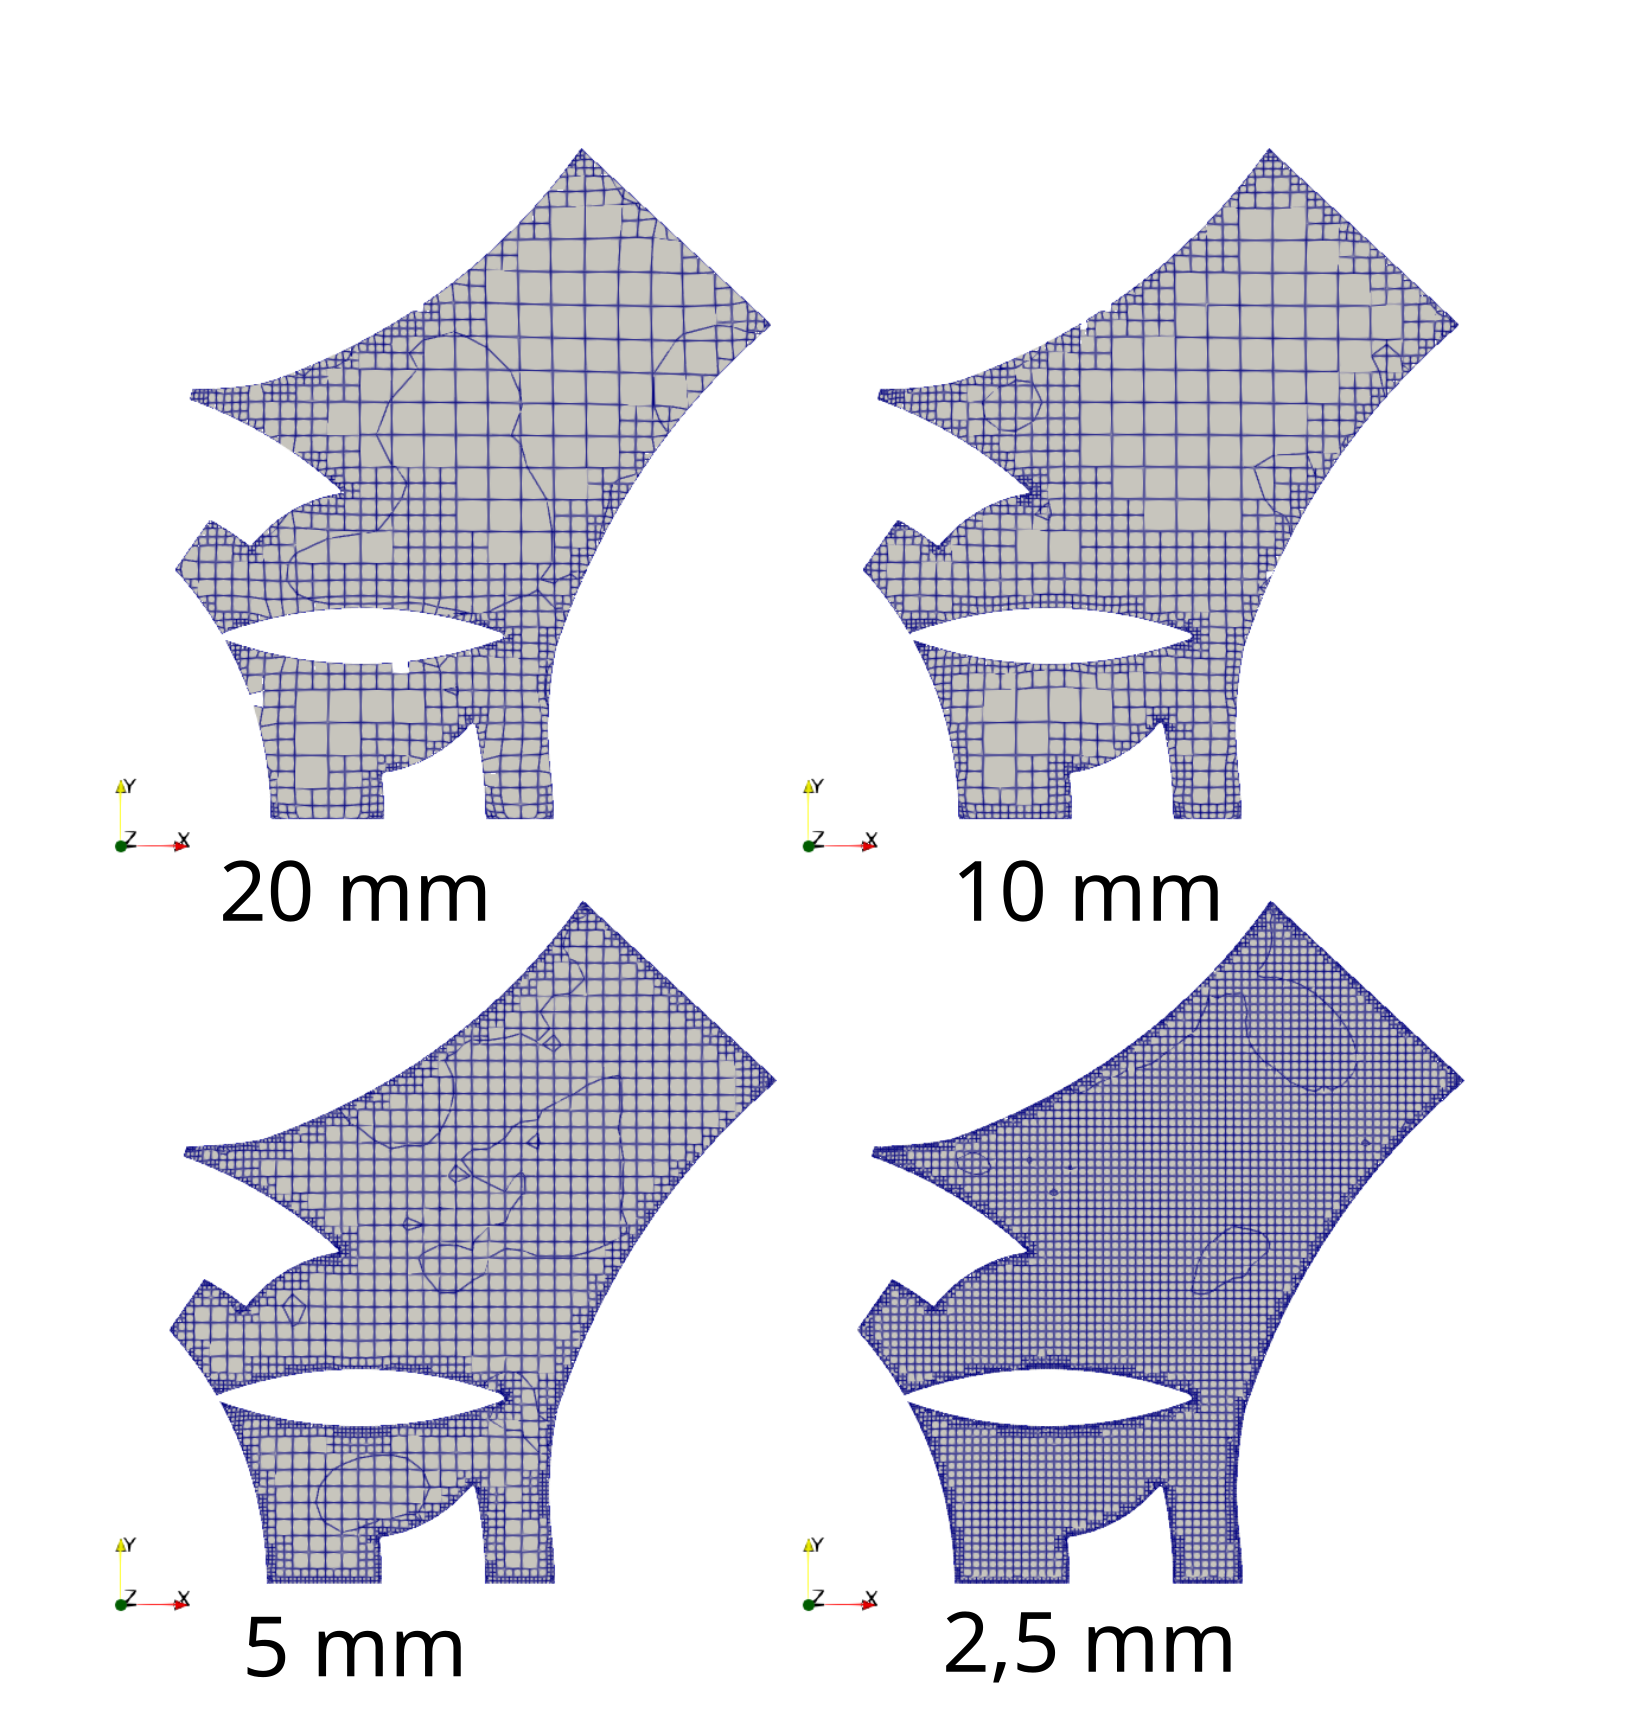
\includegraphics[width=0.8\textwidth]{./flujometrias/refinamiento_malla_escape.png}
  \caption{Refinamiento de malla para puerto de escape}\label{fig:refinamiento_escape}
\end{figure}

\begin{figure}[h]
  \centering
  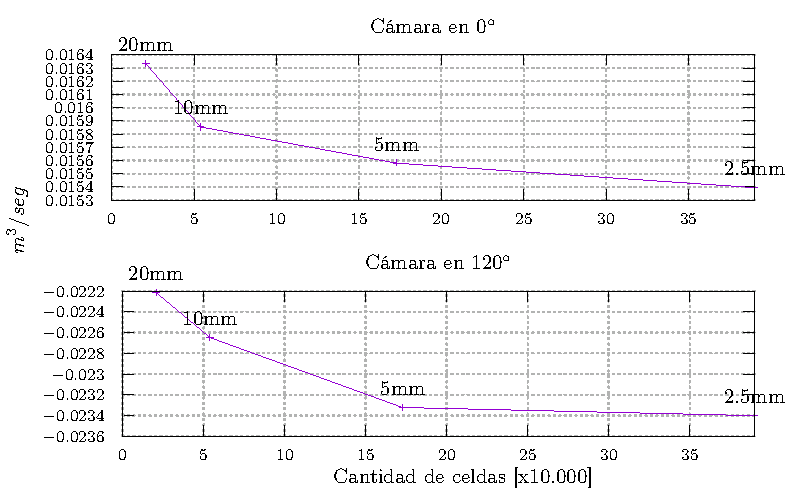
\includegraphics[width=0.9\textwidth]{./flujometrias/convergencia_admision_2000rpm.pdf}
  \caption{Convergencia de malla de puerto de admisión}\label{fig:conv_malla_admision}
\end{figure}

\begin{figure}[h]
  \centering
  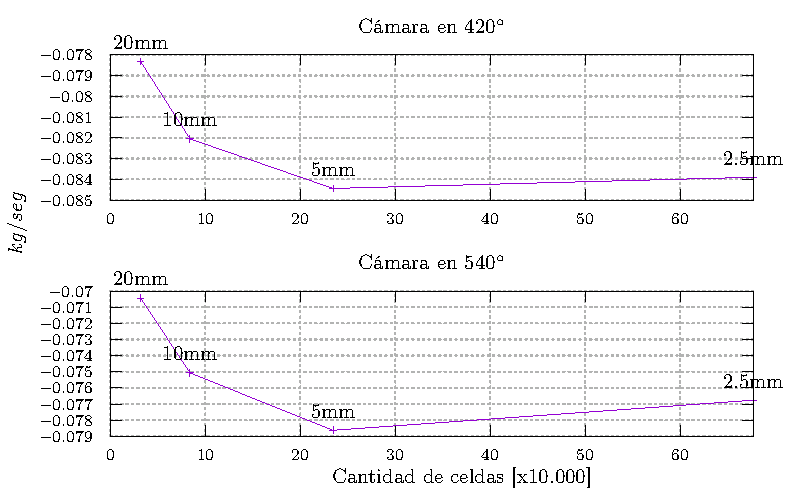
\includegraphics[width=0.9\textwidth]{./flujometrias/convergencia_escape_4000rpm.pdf}
  \caption{Convergencia de malla de puerto de escape}\label{fig:conv_malla_escape}
\end{figure}



\subsection{Esquemas de Discretización Seleccionados}

Los esquemas de discretización utilizados para los casos de \textbf{flujo incompresible} y \textbf{flujo compresible} se resumen en las siguientes tablas.

\begin{table}[h!]
    \centering
    \caption{Esquemas de discretización para flujo incompresible}
    \begin{adjustbox}{max width=\textwidth}
    \begin{tabular}{|l|l|}
        \hline
        \textbf{Componente} & \textbf{Esquema} \\ \hline
        Tiempo & Euler hacia atrás \\ \hline
        Gradiente &
        \begin{tabular}[c]{@{}l@{}}
            $\nabla p$: Integración Gaussiana con interpolación lineal \\
            $\nabla U$: Integración Gaussiana con interpolación lineal
        \end{tabular} \\ \hline
        Divergencia &
        \begin{tabular}[c]{@{}l@{}}
            $\nabla\cdot (\phi U)$: Integración Gaussiana con interpolación lineal \\
            de segundo orden, hacia adelante limitada con $\nabla U$ \\ \hline
            $\nabla\cdot (\phi k)$: Integración Gaussiana con interpolación \\
            lineal hacia adelante \\ \hline
            $\nabla\cdot (\phi \epsilon)$: Integración Gaussiana hacia \\
            adelante con interpolación lineal \\ \hline
            $\nabla\cdot (\phi R)$: Integración Gaussiana con interpolación \\
            lineal \\ \hline
            $\nabla\cdot R$: Integración Gaussiana con interpolación lineal \\ \hline
            $\nabla\cdot \nu_{eff}$: Integración Gaussiana con interpolación lineal
        \end{tabular} \\ \hline
        Laplacianos & Integración Gaussiana con interpolación lineal \\ \hline
        Interpolación & Lineal \\ \hline
        Gradientes normales a la superficie & Sin corregir \\ \hline
    \end{tabular}
    \end{adjustbox}
    \label{tab:esquemas_incompresible}
\end{table}

\begin{table}[h!]
    \centering
    \caption{Esquemas de discretización para flujo compresible}
    \begin{adjustbox}{max width=\textwidth}
    \begin{tabular}{|l|l|}
        \hline
        \textbf{Componente} & \textbf{Esquema} \\ \hline
        Tiempo & Euler \\ \hline
        Gradiente & Integración Gaussiana con interpolación lineal limitada \\ \hline
        Divergencia &
        \begin{tabular}[c]{@{}l@{}}
          $\nabla\cdot (\phi U)$: Integración Gaussiana con interpolación lineal de \\
          segundo orden, hacia adelante limitada con $\nabla U$ \\ \hline
          $\nabla\cdot (\phi, e)$: Integración Gaussiana con interpolación lineal limitada \\ \hline
          $\nabla\cdot (\phi, h)$: Integración Gaussiana con interpolación lineal hacia adelante \\ \hline
          $\nabla\cdot (\phi, p)$: Integración Gaussiana con interpolación lineal limitada \\ \hline
          $\nabla\cdot (\phi, K)$: Integración Gaussiana con interpolación lineal \\ \hline
          $\nabla\cdot (\phi, k)$: Integración Gaussiana con interpolación lineal \\ \hline
          $\nabla\cdot (\phi, \epsilon)$: Integración Gaussiana con interpolación lineal hacia adelante \\ \hline
          $\nabla\cdot (((\rho\cdot \nu_{Eff}) dev2((\nabla U)^{T})))$: Integración Gaussiana \\
          con interpolación lineal \\
        \end{tabular} \\ \hline
        Laplacianos & Integración Gaussiana con interpolación lineal, limitada y corregida \\ \hline
        Interpolación & Lineal \\ \hline
        Gradientes normales a la superficie & Corregida \\ \hline
    \end{tabular}
    \end{adjustbox}
    \label{tab:esquemas_compresible}
\end{table}

En las expresiones anteriores $\phi$ es el flujo volumétrico en la cara de la celda para flujo
incompresible y el flujo másico en la cara de la celda para flujo compresible.
%
\textbf{R} es el tensor de tensiones de Reynolds.

\section{Uso de OpenFOAM}

En esta sección se detalla la configuración, pre-procesado y detalles de la
malla utilizadas en OpenFOAM.

\subsection{Configuración}
%
Para configurar una simulación de OpenFOAM se organiza el directorio de
simulación como se indica en la Figura~\ref{fig:direc_pf} para las flujometrías
de gas considerado como incompresible  y~\ref{fig:direc_rpf} en los casos en
los que se tiene en cuenta la compresibilidad del gas.
%
Cada directorio contiene una carpeta con condiciones iniciales ``0'', malla
``constant'', configuraciones particulares de cada solver ``system'' y una
carpeta con los resultados del post-procesado el cual se puede realizar
durante cada paso de simulación o al final del proceso dependiendo de la
configuración que se haya utilizado.

\begin{figure}[h!]
  \centering
  \begin{subfigure}[b]{0.4\textwidth}
    \centering
    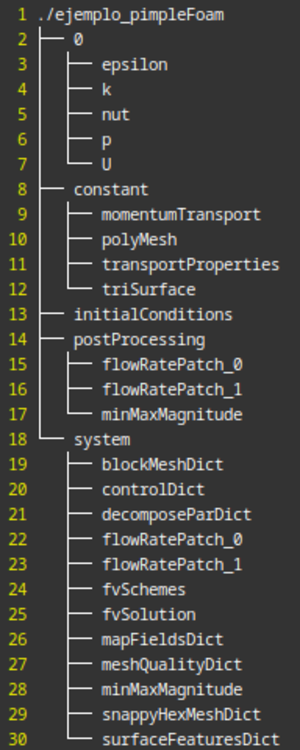
\includegraphics{flujometrias/direct_pimplefoam.pdf}
    \caption{\emph{pimpleFoam}\label{fig:direc_pf} }
  \end{subfigure}%
  \begin{subfigure}[b]{0.4\textwidth}
    \centering
    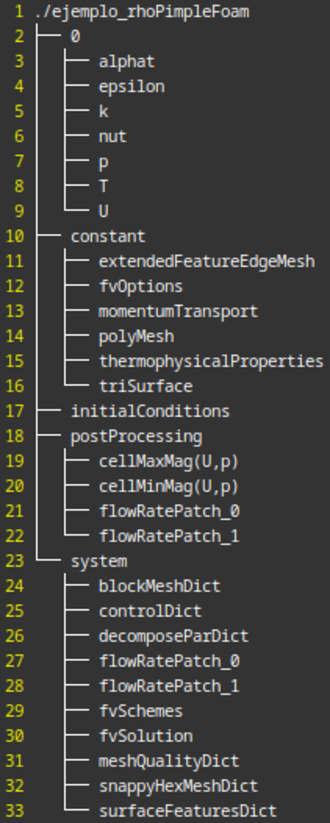
\includegraphics{flujometrias/direct_rhopimplefoam.pdf}
    \caption{\emph{rhoPimpleFoam}\label{fig:direc_rpf} }
  \end{subfigure}
  \caption{Esquema de directorios OpenFOAM}
\end{figure}


En el directorio ``0'' se indican las condiciones iniciales y de borde de cada
simulación, utilizando una configuración genérica con parámetros definidos en un
archivo separado.
%
Esto se realiza de este modo para aprovechar las características paramétricas de
OpenFOAM, permitiendo ejecutar una gran cantidad de simulaciones en serie
variando solamente los parámetros definidos en un archivo externo
``inital\_conditions.cc''.

Estos archivos de condiciones inciales se generan con un \emph{script} que toma
valores de las simulaciones de \emph{ICESym}, como se indicó en la
sección~\ref{cap2:cond_iniciales}, en la que también se detallan las ecuaciones
e hipótesis utilizadas para obtener dichos valores.
%
La ejecución de las simulaciones también se automatiza con scripts de
\emph{bash} con los pasos para ejecutar las corridas con \emph{ICESym}.
%
Con los resultados de las simulaciones se procede a calcular/leer la magnitud
del caudal másico, necesario para el cálculo del coeficiente de descarga.


\subsection{Malla}\label{sec:cap3_of_malla}
%
Una vez obtenido el archivo STL se procede a la generación de la malla dentro de
OpenFOAM con \emph{blockMesh} y \emph{snappyHexMesh}.
%
Primero se crea crea una malla con \emph{blockMesh} que  debe contener la
totalidad del volumen del puerto a simular, como se puede en la
Figura~\ref{fig:paraview_blockMesh_stl}.
%
En este paso se define el tamaño de base de la malla y el nivel general de
refinamiento.
%
A partir de estos hexaedros se produce el refinamiento por \emph{castelación}
que consiste en dividir las celdas en hexaedros más pequeños y luego aplicar el
\emph{snapping} para adaptarse a la superficie del volumen que se está
modelando, ver Figura~\ref{fig:openfoam_shm_pasos}.
%

\begin{figure}[h!]
    \centering
    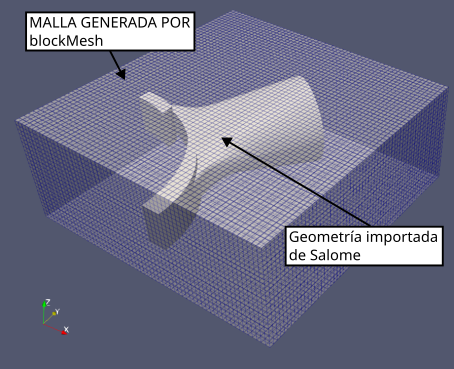
\includegraphics[width=0.5\textwidth]{flujometrias/paraview_blockMesh_stl.png}
    \caption{Malla de blockMesh y stl de Salome}\label{fig:paraview_blockMesh_stl}
\end{figure}

\begin{figure}[h!]
    \centering
    \begin{subfigure}[t]{0.5\textwidth}
        \centering
        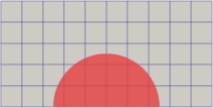
\includegraphics{flujometrias/shm_fondo.png}
        \caption{Malla de fondo y geometría}
    \end{subfigure}%
    \begin{subfigure}[t]{0.5\textwidth}
        \centering
        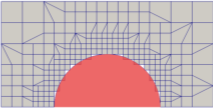
\includegraphics{flujometrias/shm_castelacion.png}
        \caption{Castelación}
    \end{subfigure}
    \begin{subfigure}[t]{0.5\textwidth}
        \centering
        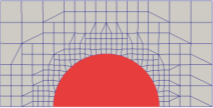
\includegraphics{flujometrias/shm_snapping.png}
        \caption{Snapping}
    \end{subfigure}
    \caption{Pasos de SnappyHexMesh\parencite{shm_steps}}\label{fig:openfoam_shm_pasos}
\end{figure}

El complemento \emph{blockMesh} crea una malla paramétrica con bloques, con
opciones para la creación de la malla con gradientes de tamaño de bloques y
diferentes opciones para los bordes, los cuales se pueden construir por líneas
rectas, arcos o
``splines''.\footnote{\url{https://doc.cfd.direct/openfoam/user-guide-v11/blockmesh}}
%
La malla se genera o configura con un diccionario \emph{blockMeshDict} ubicado
en \emph{constant/polyMesh}, con el cual se construye un cubo capaz de contener
la geometría del puerto a simular.

El complemento \emph{snappyHexMesh}
\footnote{\url{https://doc.cfd.direct/openfoam/user-guide-v11/snappyhexmesh}} es
el segundo paso del mallado.
%
Parte de una malla de bloques como la generada con la utilidad \emph{blockMesh}
y la \emph{talla} para acomodarse a la geometría dada, generando una malla 3D
conformada por hexaedros y hexaedros partidos a partir de superficies de caras
triangulares en formato de \emph{estereolitografía} (STL por sus siglas en
inglés).
%
Además permite refinar zonas particulares de la geometría y crear un
refinamiento mayor en la zona de la capa límite.

Una vez obtenido el archivo STL se procede a la generación de la malla dentro de
OpenFOAM con \emph{blockMesh} y \emph{snappyHexMesh}.
%
Primero se crea crea una malla con \emph{blockMesh} que  debe contener la
totalidad del volumen del puerto a simular, como se puede en la
Figura~\ref{fig:paraview_blockMesh_stl}.
%
En este paso se define el tamaño de base de la malla y el nivel general de
refinamiento.
%
A partir de estos hexaedros se produce el refinamiento por \emph{castelación}
que consiste en dividir las celdas en hexaedros más pequeños y luego aplicar el
\emph{snapping} para adaptarse a la superficie del volumen que se está
modelando, ver Figura~\ref{fig:openfoam_shm_pasos}.
%

\subsection{Pre-procesado}
%
El preprocesado consiste en definir geometría y condiciones iniciales de la
simulación a partir de los datos obtenidos de las simulaciones con el
optimizador e ICESym.
%
Con los resultados del simulador se grafica la diferencia de presión entre el
puerto de admisión o escape y la cámara correspondiente en función de la apertura
del puerto, para un rango de velocidades de 1000 a 9000 RPM, con el fin de
identificar las zonas en las condiciones operativas en las que evaluar el puerto.
%
En la Figura~\ref{fig:puntos_interes} se muestra una gráfica de $\Delta P$ y
alzada para los puertos de admisión y escape de 1000 a 4000 RPM de un motor
resultante de una de las simulaciones.

Como es de esperarse se tienen mayores diferenciales de presión a menores
aperturas del puerto porque se está próximo a los eventos de apertura o cierre
del mismo.
%
A diferencia del puerto de admisión, en el puerto de escape se ve una banda
bastante definida de operación que se hace más ``llena'' a medida que aumenta la
apertura del puerto.
%
Durante la apertura del puerto se ven las mayores diferencias de presión en las
que hay dos bandas bien definidas.
%
Se toman algunos puntos arriba en la zona con mayor $\Delta P$ y una cantidad
menor para velocidades con $\Delta P \simeq 0$.
%
A medida que el puerto se abre la diferencia de presión con el gas en la cámara
disminuye y esta banda se afina.

\begin{figure}[h!]
    \centering
    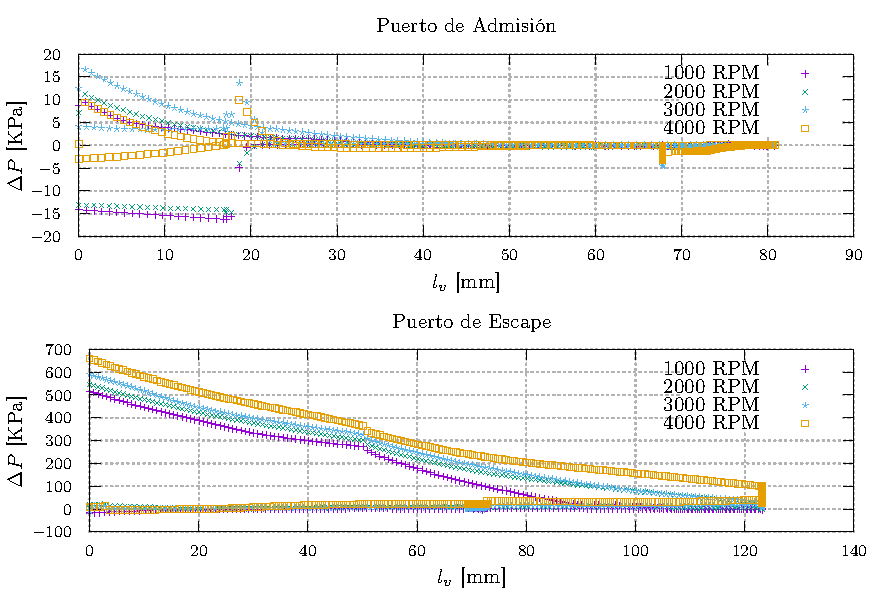
\includegraphics[width=\textwidth]{gnuplot/puntos_interes.pdf}
    \caption{Presión en función de la apertura el puerto,
$\Delta P = f(l_{v})$}\label{fig:puntos_interes}
\end{figure}

El valor de alzada está directamente relacionado con la posición angular del
cigüeñal, por lo que una vez seleccionados los puntos de interés se puede
extraer la geometría deseada de un modelo de CAD paramétrico del motor.
%
En este modelo se representó la mitad de la geometría que contiene los puertos
de admisión y escape, y se obtuvo realizando operaciones geométricas con los
volúmenes que representan diferentes componentes del motor como son el estator,
rotor, paletas, etc.


\begin{figure}[h!]
    \centering
    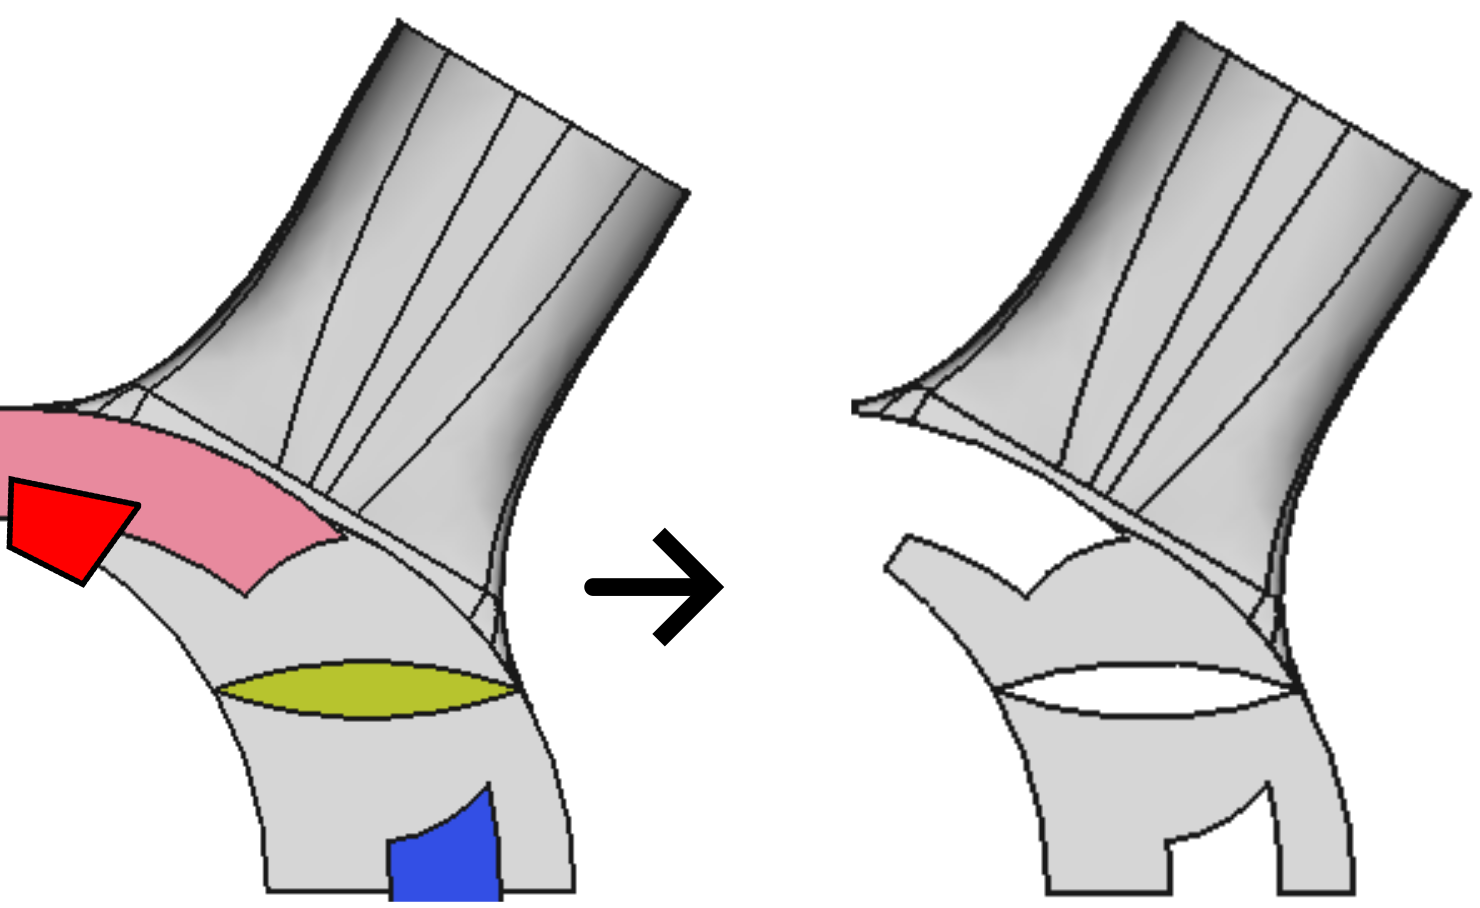
\includegraphics[width=0.7\textwidth]{./CAD/freecad_pasos.png}
    \caption{Puerto de admisión para $\theta=50^{\circ}$ modelado con
FreeCAD}\label{fig:admision_50}
\end{figure}

Esta geometría fue generada por el programa FreeCAD~\parencite{freecad},
exportada a un archivo
``.BREP''\footnote{\href{https://dev.opencascade.org/doc/overview/html/specification\_\_brep\_format.html}{Formato
BREP, opencascade.org}} para luego ser importada en Salome\parencite{salome},
que se utiliza para generar una malla cerrada, hermética, que puede ser
procesada por los complementos de OpenFOAM utilizados para generar la malla de
la simulación.
%
Es importante que se satisfaga la hermeticidad de la malla, lo cual significa
que los nodos en la frontera entre superficies coincidan, como se puede observar
en la Figura~\ref{fig:salome_malla_hermetica}, en la que se ven dos superficies
``walls'' y ``outlet'' y los nodos compartidos entre ambas superficies.
%

\begin{figure}[h!]
    \centering
    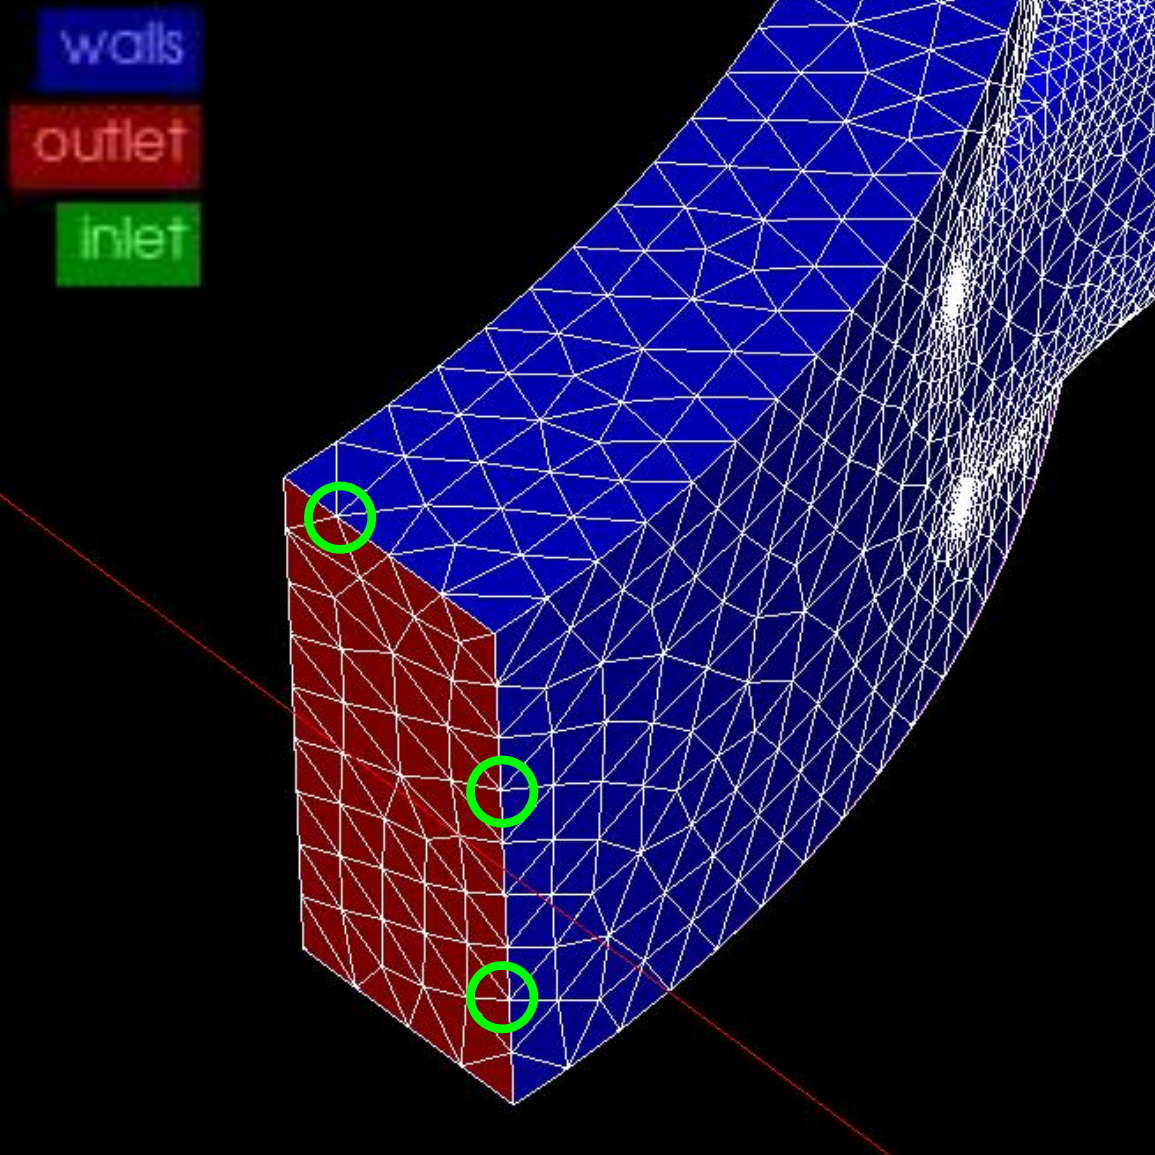
\includegraphics[width=0.4\textwidth]{./flujometrias/salome_malla_hermetica.png}
    \caption{Malla hermética}\label{fig:salome_malla_hermetica}
\end{figure}

El proceso en Salome consta de importar la geometría generada por FreeCAD y
separar la misma en superficies utilizadas para definir condiciones de contorno
en OpenFOAM.
%
Las superficies diferenciadas son: puerto, cámara/s y pared, ver
Figura~\ref{fig:openfoam_parches}.

\begin{figure}[h!]
    \centering
    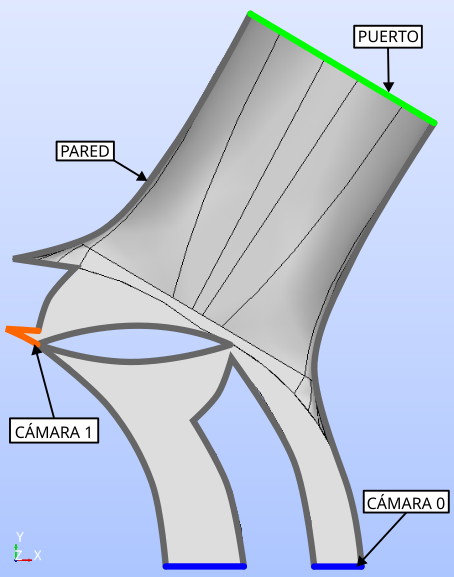
\includegraphics[width=0.5\textwidth]{./flujometrias/openfoam_parches.png}
    \caption{Nombres de Parches}\label{fig:openfoam_parches}
\end{figure}

Luego de separadas estas superficies se procede a generar la malla en formato
ASCII STL con el complemento de mallado de Salome.
%
Se utilizó el generador de mallas NETGEN 1D-2D para crear la superficie, en
general se configuró el software de modo de tener un stl de buena calidad con
elementos de menor tamaño en zonas de mayor curvatura.
%
En la Figura~\ref{fig:salome_fina_gruesa} se ve la diferencia en cantidad de
nodos de dos mallas, una malla fina a la izquierda y una malla gruesa a la
derecha.
%
En la Tabla~\ref{tab:salome_fina_gruesa} se muestra la diferencia entre algunos
parámetros básicos de configuración para las dos mallas.
%
% Esto sin requerir de una gran cantidad de elementos para no ralentizar el
% procesado con SnappyHexMesh.

\begin{figure}[h!]
    \centering
    \begin{subfigure}[t]{0.5\textwidth}
        \centering
        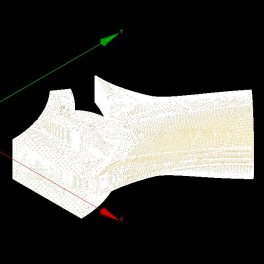
\includegraphics{/flujometrias/salome3_fina.png}
        \caption{Malla fina sin optimizar}
    \end{subfigure}%
    \begin{subfigure}[t]{0.5\textwidth}
        \centering
        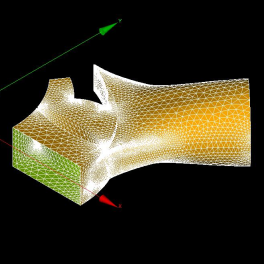
\includegraphics{/flujometrias/salome3_gruesa.png}
        \caption{Malla gruesa optimizada}
    \end{subfigure}
    \caption{Diferentes mallas para flujometrías}\label{fig:salome_fina_gruesa}
\end{figure}

\begin{table}[h!]
    \centering
    \begin{tabular}{lccc} \toprule
        Parámetro                & Malla Fina    & Malla Gruesa     & Unidades\\ \midrule
        Tamaño máximo            & 0,001         & 0,03             & m \\
        Tamaño mínimo            & 1E-7          & 2,4E-5           & m \\
        Limitado por curvatura   & Sí            & Sí               & - \\
        Optimizar                & No            & Sí               & - \\
        Cantidad de nodos        & 99311         & 49112            & - \\
        Cantidad de elementos    & 204695        & 103163           & - \\ \bottomrule
    \end{tabular}
    \caption{Configuración de mallas mostradas en la Figura~\ref{fig:salome_fina_gruesa}}
    \label{tab:salome_fina_gruesa}
\end{table}
 \pagebreak

\chapter{RESULTADOS}\label{capitulo:RESULTADOS}
Los resultados obtenidos en cada uno de los pasos de este trabajo se detallan en
este capítulo, comenzando por el motor obtenido en la primera iteración de
optimización con el algoritmo genético junto con el modelo geométrico 3D
generado.
%
Luego se muestran los resultados de las flujometrías realizadas a partir del
modelo de CAD, incluyendo las mallas obtenidas para algunos casos seleccionados
y el resultado detallado de algunas de las flujometrías, finalizando con el mapa
de $C_{D}$ obtenido, tanto para el puerto de admisión como para
el puerto de escape.

Por último se presentan los resultados de la segunda ronda de optimización con
el algoritmo genético, en la que se utilizó el mapa de $C_{D}$ obtenido en el
paso previo.

\section{Primera Iteración}
%
La primera optimización se realizó partiendo de una población al azar, con los
coeficientes de descarga constantes de 0,7 y 0,75 para el puerto de admisión y
escape respectivamente.
%
El algoritmo genético se ejecutó durante 20 generaciones con una población de
100 individuos y la función objetivo definida en la
sección~\ref{sec:funcion_objetivo} con los pesos, operadores y
parámetros correspondientes indicados en la Tabla~\ref{tab:config_genetico}.

\begin{table}[h!]
  \centering
  \begin{tabular}{ccc} \toprule
    Parámetro & Valor & Unidad \\ \midrule
    RPMS & $1000\times[1, 2, 3, 4, 5, 6, 7, 8, 9]$ & \\
    Pesos de función objetivo & $(1, 1, 1, 6, 8, 9, 8, 7, 7)$ & \\
    Diámetro mínimo & 0,05 & m \\
    Diámetro máximo & 0,1 & m \\
    Longitud mínima de tubo & 0,5 & m \\
    Longitud máxima de tubo & 2 & m \\
    Ángulo mínimo & 0 & grados \\
    Ángulo máximo & 90 & grados \\
    Separación angular máxima & 70 & grados \\
    Tamaño de población & 100 & - \\
    Tamaño de torneo & 10 & - \\
    Probabilidad de cruza & 0,9 & - \\
    Probabilidad de mutación & 0,5 & - \\
    Cantidad de generaciones & 20 & - \\
    Tamaño de \emph{SALÓN DE LA FAMA} & 1 & - \\ \bottomrule
    \end{tabular}
  \caption{Configuración utilizada.}\label{tab:config_genetico}
\end{table}

% Nota: terminar de agregar la figura
% Para ICESym se utilizaron dos ciclos de simulación, por considerarse que es
% suficientemente preciso para esta primer aproximación.
%
% En la Figura XX se puede ver que a partir de la segunda iteración se obtienen
% buenos resultados, esto se debe a que los datos de partida para la segunda
% iteración, son los resultados de la primer iteración.
%

En la Figura~\ref{fig:ev_primer_op}, donde se representa la evolución de la
población tras iteraciones sucesivas, se observa que se obtuvo rápidamente un
individuo con un puntaje relativamente alto en las primeras iteraciones.
%
El resultado final tiene una aptitud 1.5 veces la aptitud media de la población
de la última generación, siendo los parámetros que definen este candidato los
listados en la Tabla~\ref{tab:resultado_primer_it} y cuyos indicadores se
ilustran en la Figura~\ref{fig:primer_op}.
%
Este motor tiene un rendimiento volumétrico máximo de $\eta_{v} \simeq 0.83$
para 2500 RPM y si bien la función objetivo favorece curvas suaves, se ven dos
picos de rendimiento en la curva, siendo el segundo con $\eta_{v} \simeq 0.79$ a
7500 RPM.

A modo de comparación, en la misma Tabla se presentan las características
geométricas obtenida en trabajos anteriores~\parencite{mrcvc_geom}.

\begin{figure}[h!]
  \centering
  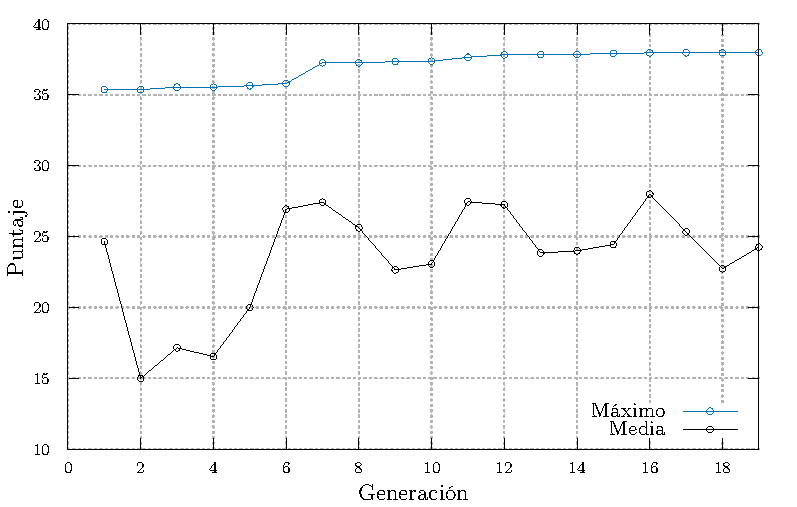
\includegraphics[width=.8\textwidth]{gnuplot/genetico.pdf}
  \caption{Evolución de la población} \label{fig:ev_primer_op}
\end{figure}%
\begin{figure}[h!]
  \centering
  \includegraphics[width=.8\textwidth]{gnuplot/primer-rendimiento.pdf}
  \caption{Rendimiento volumétrico y fracción de gases residuales del motor seleccionado} \label{fig:primer_op}
\end{figure}

% TODO revisar los ángulos de los puertos
\begin{table}[h!]
  \centering
  \begin{tabular}{ccccc} \toprule
    Parámetro & \multicolumn{2}{c}{Admisión} & \multicolumn{2}{c}{Escape} \\ \cmidrule(lr){2-3} \cmidrule(lr){4-5} & Inicial & Final & Inicial & Final \\
    \midrule
    Longitud del tubo [mm]               & 1300   & 519    & 800    & 976  \\
    Diámetro del tubo [mm]               & 70     & 97     & 50     & 81   \\
    Ángulo de apertura del puerto [grad] & 592.93 & 584.05 & 396.87 & 396.69 \\
    Ángulo de cierre del puerto [grad]   & 175.76 & 182.74 & 587.06 & 5.95 \\
    \bottomrule
  \end{tabular}
  \caption{Datos geométricos del mejor candidato}
  \label{tab:resultado_primer_it}
\end{table}


En la Figura~\ref{fig:PoTi_primer_op} se muestran las curvas de potencia y
torque del motor.
%
Como es de esperarse se ve que ambas están directamente condicionadas por el
rendimiento volumétrico, con una potencia al freno máxima de 177 CV a 7500 RPM y
un torque máximo de 191 N.m a\ 2500 RPM.

\begin{figure}[h!]
  \centering
  \includegraphics[width=\textwidth]{gnuplot/primer-potencia.pdf}
  \caption{Torque y Potencia de Primera Iteración} \label{fig:PoTi_primer_op}
\end{figure}


\section{Modelo de CAD}
%
A partir de los resultados obtenidos se realizó un modelo de CAD de los puertos
que se ilustra en las Figuras~\ref{fig:motor_cad1} y~\ref{fig:motor_cad2}.
%
Se representó solamente la mitad superior del motor que contiene los puertos
de admisión y escape.
%
Este modelo es paramétrico y permite rotar los componentes del motor para
obtener distintas posiciones del conjunto y así poder generar la geometría a
evaluar con las flujometrías.

% Algunos redondearon las aristas internas incluyendo las paletas y las puntas del rotor para favorecer el proceso de mallado, ya que los bordes agudos pueden ser problmeáticos para el mallador \emph{snappyHexMesh}.

\begin{figure}[h!]
  \centering
  \subfloat[]{
    \includegraphics[width=.5\textwidth]{CAD/motor_cad1.png}
  }
  \subfloat[]{
    \includegraphics[width=.5\textwidth]{CAD/motor_cad2.png}
  }
  \caption{CAD Primera iteración}\label{fig:motor_cad1}
\end{figure}


\begin{figure}[h!]
  \centering
  \subfloat[Puerto de Admisión]{
    \includegraphics[width=\textwidth]{CAD/vistas_admision.png}
  }
  \hfill
  \subfloat[Puerto de Escape]{
    \includegraphics[width=\textwidth]{CAD/vistas_escape.png}
  }
  \caption{CAD Primera iteración (vistas fuera de escala).}\label{fig:motor_cad2}
\end{figure}

La altura del puerto del lado de la cámara se mantuvo en dos tercios de la
altura de la cámara $h_{p} = \frac{2}{3}h_{c}$, manteniendo el eje central de cada
puerto de forma que intersecte el centro del motor con el propósito de eliminar
una variable de la geometría a modelar.
%
El foco de esta etapa de optimización es el diámetro del puerto y el reglaje.
%

%%%%%%%%%%%%%%%%%%%%%%%%%%%%%%%%%%%%%%%%%%%%%%%%%%%%%%%%%%%%%%%%%%%%%%%%%%%%%%%

\section{Flujometrías}

De la primera iteración se obtuvo la geometría y datos operativos del motor, lo
cual permitió representar la curva de diferencia de presión ($\Delta P$) en
función de la alzada ($l_{v}$) de ambos puertos para diferentes velocidades de
giro, identificando los puntos de mayor interés en los cuales realizar las
flujometrías.
%
Los pares $(l_{v}, \Delta P)$ seleccionados para modelar el flujo del puerto se
detallan en las Figuras~\ref{fig:delta_p_admision} y~\ref{fig:delta_p_escape}.
%
Inicialmente se propusieron 51 flujometrías pudiendo realizar un total de 36
simulaciones que devolvieron 56 valores de $C_{D}$.

\begin{figure}[h!]
  \centering
  \includegraphics[width=\textwidth]{flujometrias/admision_delta_p_anot.png}
  \caption{Flujometrías puerto de admisión}\label{fig:delta_p_admision}
\end{figure}

\begin{figure}[h!]
  \centering
  \includegraphics[width=\textwidth]{flujometrias/escape_delta_p_anot.png}
  \caption{Flujometrías puerto de escape}\label{fig:delta_p_escape}
\end{figure}


Algunas flujometrías se realizaron en tres etapas, partiendo de una malla gruesa
con celdas de $15$ mm de tamaño inicial y culminando en celdas de $5$ mm.
%
En otros se realizó directamente la flujometría con mallas base de $5$ mm.

En general se simularon alrededor de $0,02$ segundos de flujado, suficiente para
alcanzar un valor estable del caudal, como se ejemplifica en la
Figura~\ref{fig:adm_10_7000rpm}, donde se muestra el desarrollo de la simulación
en términos de $\dot{Q}$ para el puerto de admisión con el cigüeñal en
$\theta=10^{\circ}$.
%
Para esta flujometría en particular se tiene un flujo de los gases desde la
cámara hacia el puerto de admisión, correspondiente a un puerto que abre.

%
% La línea anaranjada sobre el final de la simulación representa la porción de
% datos que se seleccionó para calcular $\dot{m}$, lo cual se realizó tomando la
% media de los últimos $n$ valores obtenidos de los resultados de las flujometrías
% para los puertos de admisión y escape, las cuales se presentan en el
% Anexo~\ref{anexo:1}.
%

\begin{figure}[h!]
  \centering
  \includegraphics[width=0.7\textwidth]{./gnuplot/puerto_admision_10_7000.pdf}
  \caption{Puerto de admisión $10^{\circ}$ \@ $7000$ RPM}\label{fig:adm_10_7000rpm}
\end{figure}

Como se mencionó en la introducción del capítulo~\ref{capitulo:DESARROLLO}, la
modificación realizada a ICESym para funcionar con un mapa de $C_{D}$
dependiente de dos variables requiere que los datos de entrada estén
distribuidos en una grilla rectangular.
%
Se utilizó entonces un método de interpolación de punto más cercano suavizado
por promedio móvil con $S=2$ para generar dicha grilla a partir de los puntos
conocidos de $C_{D}$.
%
El resultado puede observarse en las Figuras~\ref{fig:mapa_cd_admision}
y~\ref{fig:mapa_cd_escape}.
%
Con respecto al gradiente de presión indicado en las figuras que se presentan en
los párrafos siguientes, para ambos puertos se define el gradiente de presión
como la diferencia entre la presión en la cámara y la presión en el puerto,
$\Delta P = P_{\text{c\'amara}} - P_{\text{puerto}}$.
%
En la Tabla~\ref{tab:resumen_puertos} se resumen los valores máximos y mínimos
de $C_{D}$ y $\dot{m}$ obtenidos para los puertos de admisión y escape.

\begin{table}[h!]
  \centering
  \begin{tabular}{cccccccc}\toprule
    Puerto   & $l_{v} [mm]$ & $\Delta P [kPa]$ & $C_{D}$ & $\dot{m} [g/seg]$ & Nota            & Figura\\ \midrule
    Admisión & 62,95        &  7,4            & 0,59   & -122              & $C_{D,\max}$     &\ref{fig:adm_cd_max} \\
    Admisión & 81,94        &  -4,95           & 0,32   &   70              & $\dot{m}_{\max}$ &\ref{fig:adm_cd_max} \\
    Escape   & 87,76        & 10,7            & 0,58   &  145              & $C_{D,\max}$     &\ref{fig:esc_cd_max}\\
    Escape   & 87,76        & 33,4            & 0,45   &  176              & $\dot{m}_{\max}$ &\ref{fig:esc_m_max}\\ \bottomrule
  \end{tabular}
  \caption{Valores máximos $C_{D}$ y $\dot{m}$ para puertos}\label{tab:resumen_puertos}
\end{table}


\subsection{Puerto de Admisión}
%
En el mapa del coeficiente de descarga para el puerto de admisión
(Fig.\ref{fig:mapa_cd_admision}) se pueden observar en rojo las zonas de menor
eficiencia del escurrimiento.
%
Esto ocurre para posiciones relacionadas con la apertura y cierre del puerto
donde las presiones y velocidades de flujo involucradas son mayores, aumentando
las pérdidas de carga.
%
La misma tendencia se observa si se representa el $C_{D}$ en función de la
apertura del puerto $l_{v}$ o del gradiente de presión $\Delta P$, ver
Figura~\ref{fig:cd_admision}.
%
Los mayores valores de $C_{D}$ ocurren para la mayor apertura o, en general,
para el menor gradiente de presión en términos absolutos.
%
También se observa que el coeficiente de descarga medio para el puerto es
aproximadamente $0,3$.

\begin{figure}[h!]
    \centering
    \includegraphics[width=0.7\textwidth]{mapa_cd/heatmap_cda.png}
    \caption{Mapa de $C_{D}$ del puerto de admisión}\label{fig:mapa_cd_admision}
\end{figure}

\begin{figure}[h!]
    \centering
    \includegraphics{gnuplot/cd_vs_alzada_adm.pdf}
    \caption{$C_{D}$ del puerto de admisión}\label{fig:cd_admision}
\end{figure}

El máximo coeficiente de descarga vale $C_{D,\max}\simeq 0,6$ para
$l_{v}=62,95 mm$ y $\Delta P\simeq +7,37 KPa$, obteniendo un flujo saliente del
puerto de $122,09 g/seg$.
%
Para este caso se observa un reflujo de gases residuales apenas abre el puerto
de admisión, correspondiendo a un ángulo de cigüeñal de $10^{\circ}$ a $7000$
RPM.


La flujometría correspondiente al último instante de la simulación se muestra en
la Figura~\ref{fig:adm_cd_max}, en la cual las líneas de corriente están
coloreadas según el módulo de la velocidad y las flechas indican el sentido de
flujo.
%
La mayor velocidad del flujo se da en el gas que sale de la cámara,
correspondiente a masa residual atrapada luego del barrido del puerto de escape.

El flujo másico máximo hacia adentro de la cámara ($\Delta P<0$) ocurre para la
misma geometría indicada en la Figura~\ref{fig:adm_cd_max}.
%
Se alcanza $\dot{m}_{\max}\simeq 70 g/seg$ para la cámara que se encuentra más
avanzada en el proceso de admisión y con máxima apertura del puerto con $l_{v}=81,94 mm$ y $\Delta P=-4,95 KPa$ siendo $C_{D}\simeq 0,32$.

\begin{figure}[h!]
    \centering
    \includegraphics[width=\textwidth]{flujometrias/adm_cd_max.png}
    \caption{Admisión - Máximo $C_{D}$}\label{fig:adm_cd_max}
\end{figure}


\subsection{Puerto de Escape}
%
En la Figura~\ref{fig:mapa_cd_escape} se ilustra el mapa de $C_{D}$ obtenido para el
puerto de escape donde la tendencia es similar al puerto de admisión.
%
En la Figura~\ref{fig:cd_escape} se observa que el coeficiente de descarga es
mayor para aperturas mayores del puerto y menores gradientes de presión
($|\Delta P|\sim 0$).



\begin{figure}[h!]
    \centering
    \includegraphics[width=.7\textwidth]{mapa_cd/heatmap_cde.png}
    \caption{Mapa de $C_{D}$ del puerto de escape}\label{fig:mapa_cd_escape}
\end{figure}

\begin{figure}[h!]
    \centering
    \includegraphics{gnuplot/cd_vs_alzada_esc.pdf}
    \caption{$C_{D}$ del puerto de escape}\label{fig:cd_escape}
\end{figure}

El máximo coeficiente de descarga obtenido vale $C_{D,\max}\simeq 0,58$ y ocurre
para $l_{v}=87,76 mm$, $\Delta P=10,7 KPa$ con un flujo másico de $145 g/s$
hacia afuera para $440^{\circ}$ a $9000$ RPM.
%
Por otro lado el máximo caudal másico es $\dot{m}=176,1 g/seg$ y ocurre para
$l_{v}=87,76 mm$ y $\Delta P=334 KPa$, correspondiendo a $440^{\circ}$ y 7000
RPM.
%
La flujometría correspondiente al valor máximo de $C_{D}$ se muestra en la
Figura~\ref{fig:esc_cd_max}.
%
% Las líneas de corriente muestran una gran diferencia de velocidad entre el gas
% que escapa por las paredes externas del puerto en comparación al que debe
% escurrir entre las paletas y el rotor.

\begin{figure}[h!]
    \centering
    \includegraphics[width=\textwidth]{flujometrias/esc_cd_max.png}
    \caption{Escape - Valor máximo de $C_{D}$}\label{fig:esc_cd_max}
\end{figure}

La flujometría correspondiente al valor máximo de flujo másico obtenido, se
muestra en la Figura~\ref{fig:esc_m_max}.

\begin{figure}[h!]
    \centering
    \includegraphics[width=\textwidth]{flujometrias/esc_m_max.png}
    \caption{Escape - Valor máximo de $\dot{m}$}\label{fig:esc_m_max}
\end{figure}

%%%%%%%%%%%%%%%%%%%%%%%%%%%%%%%%%%%%%%%%%%%%%%%%%%%%%%%%%%%%%%%%%%%%%%%%%%%%%%%%
%%%%%%%%%%%%%%%%%%%%%%%%%%%%%%%%%%%%%%%%%%%%%%%%%%%%%%%%%%%%%%%%%%%%%%%%%%%%%%%%
%%%%%%%%%%%%%%%%%%%%%%%%%%%%%%%%%%%%%%%%%%%%%%%%%%%%%%%%%%%%%%%%%%%%%%%%%%%%%%%%

\section{Segunda Iteración y Resultado Final}
%
En la segunda iteración se utilizó el mapa de $C_D$ para la admisión y escape
como dato de entrada de ICESym.
%
Con estos nuevos datos se realizó una serie de corridas de optimización con el algoritmo
genético, de las cuales se seleccionaron los mejores candidatos.
%
Se obtuvieron los candidatos cuyas geometrías se listan en la
Tabla~\ref{tab:2iter_geom}.
%
Los diámetros de los conductos de admisión son similares en todos los casos,
mientras que para el escape se tiene un par con conductos de 63 mm y otro con
95 mm.
%
La mayor variación ocurre en los largos de los conductos y los ángulos de apertura y
cierre.
%
Para seleccionar uno de los candidatos, se compararon las curvas de rendimiento
volumétrico, torque, potencia y fracción de gases residuales de estos motores,
las cuales se muestran en la Figura~\ref{fig:comparativa_segunda_iter}.

\begin{table}[h!]
  \centering
  \begin{tabular}{ccccccccc}\toprule
    Corrida   & DTA   & DTE & LIT   & LET   & IIA   & IFA   & EIA    & EFA \\
    -         & [mm] & [mm] & [m]   & [m]   & [gra] & [gra] & [gra]  & [gra] \\ \midrule
    run 3-4   & 99   & 63   & 0,839 & 0,79  & 3,23 & 60,0   & 78,39  & 36,29 \\
    run 5-4   & 90   & 95   & 0,742 & 0,597 & 8,39 & 60,0   & 68,23  & 23,23 \\ \bottomrule
    % run 09-04 & 82   & 91   & 0,79  & 1,758 & 3,23 & 60,97  & 75,48  & 39,19 \\
    % run 10-04 & 96   & 60   & 1,129 & 1,468 & 6,13 & 66,78  & 62,42  & 40,65 \\ \bottomrule
  \end{tabular}
  \caption{Geometrías de segunda iteración}\label{tab:2iter_geom}
\end{table}

\begin{figure}[h!] \centering
\includegraphics[width=\textwidth]{gnuplot/comparativa_segunda_iter_mep.pdf}
  \caption{Comparativa de candidatos} \label{fig:comparativa_segunda_iter}
\end{figure}

En base a esta comparativa se optó por seleccionar la corrida denominada como
``run 3-4''

% , este motor presenta un máximo de torque y potencia en 2500 RPM,
% también presenta una curva de rendimiento volumétrico suave con un máximo en
% 2500 RPM.
%
% En términos de potencia mantiene valores elevados a partir del cercanos a los
% 130 CV.
%
En todos los candidatos se observa una alta fracción de gases residuales a altas
RPM y una disminución notoria del rendimiento volumétrico.

El motor tiene una potencia máxima de 113 CV a las 5000 RPM que se mantiene
plana hasta las 7000 RPM.
%
En cuanto al par motor, se tiene el máximo de 180 Nm a 2500 RPM y se mantiene
por encima de 160 Nm hasta las 5000 RPM.
%
Este coincide con el máximo de rendimiento volumétrico de $\sim 0,845$.
%
En la Figura~\ref{fig:PoTi_segunda_op} se notan los efectos del coeficiente de
descarga en la simulación del motor, comparando los resultados de la primera
iteración con coeficientes de descarga constantes a la segunda con el mapa de
$C_{D}$ en función de la presión y grado de apertura del puerto.

\begin{figure}[h!]
  \centering
  \includegraphics{gnuplot/comparativa.pdf}
  \caption{Comparativa de Torque y potencia al freno} \label{fig:PoTi_segunda_op}
\end{figure}
 \pagebreak

\chapter{CONCLUSIONES}\label{capitulo:CONCLUSIONES}
Se ha obtenido un prediseño de los sistemas de admisión y escape que buscó
maximizar el rendimiento volumétrico y reducir la fracción de gases residuales
en un rango medio a medio alto de revoluciones del motor, obteniendo una curva
de rendimiento volumétrico con dos máximos locales a 2500 y 5000 RPM,
manteniendo valores de  $\eta_v$ mayores al 60\% hasta 8000 RPM.
%
Además, se obtuvo un mapa de $C_D$ que modeliza el funcionamiento de los
puertos con apertura de puerto y diferencia de presión como variables.

Junto con estos resultados se desarrolló un conjunto de \emph{scripts} que
permiten utilizar el simulador ICESym como una \emph{caja negra}, pudiendo
configurar, ejecutar y leer los resultados de una simulación, permitiendo
utilizar el simulador acoplado a otro programa.

Por otro lado, se pudieron comparar los resultados del simulador utilizando un valor
de $C_{D}$ constante en lugar de utilizar un mapa de $C_{D}$ en función de
valores de presión y apertura del puerto.

Como posible trabajo a futuro se propone continuar con el proceso de optimización
que se inició en este trabajo, realizando más iteraciones para refinar la
geometría obtenida.
%
Otro aspecto a trabajar a futuro es reducir la cantidad de gases residuales que
se producen por efecto del solape de cámaras.
%
Así como también explorar otras funciones objetivo para la optimización con el
algoritmo genético.
 \pagebreak

\chapter{REFERENCIAS}
\printbibliography[heading=none] \pagebreak

\chapter{ANEXO I}


 
 \pagebreak


%Esta línea fuerza a colocar en Referencias las que no fueron citadas en el texto
%\nocite{*}

%Imprime bibliografia del archivo biblio.bib
\printbibliography[heading=none]
